%% Journal of Systems and Software -- Special Issue on Software Engineering for
%% Trustworthy Systems and Advanced Applications.
%% Elsevier CAS template, single column (cas-sc). Single-file manuscript:
%% all tables, figures and generated numbers are inlined.
%% Build: pdflatex main; bibtex main; pdflatex main; pdflatex main
\documentclass[a4paper,fleqn]{cas-sc}
\usepackage[authoryear]{natbib}
\usepackage{amsthm}
\usepackage{tikz,pgfplots}
\usepackage{algorithm}
\usepackage[noend]{algpseudocode}
\usepackage{textcomp}
\usepackage{url}
\usepackage{listings}
\usepgfplotslibrary{groupplots}
\usetikzlibrary{arrows.meta,positioning,fit,calc,automata,backgrounds}
\pgfplotsset{compat=1.18}
\newcommand{\todo}[1]{\textcolor{red}{[TODO: #1]}}

\definecolor{inkblue}{RGB}{31,70,104}
\definecolor{pale}{RGB}{239,245,249}
\definecolor{resultteal}{RGB}{23,130,132}
\definecolor{resultamber}{RGB}{216,126,45}
\pgfplotsset{vgcplot/.style={font=\scriptsize,label style={font=\footnotesize},tick label style={font=\scriptsize},
  axis line style={draw=inkblue!45},tick style={draw=inkblue!35},xmajorgrids=true,ymajorgrids=true,
  grid style={draw=gray!18},legend style={font=\scriptsize}}}
\tikzset{box/.style={draw=inkblue,rounded corners=2pt,fill=pale,align=center,minimum height=7mm,font=\footnotesize},
  arr/.style={-{Stealth[length=2mm]},thick,draw=inkblue}}
\newenvironment{steps}{\begin{list}{}{\setlength{\leftmargin}{1.9em}\setlength{\labelwidth}{1.4em}\setlength{\labelsep}{0.5em}\setlength{\itemsep}{1pt}}}{\end{list}}
\newcommand{\step}[1]{\tikz[baseline=(c.base)]\node[circle,draw=inkblue,line width=0.6pt,fill=white,text=inkblue,inner sep=0pt,minimum size=3.6mm,font=\scriptsize\sffamily\bfseries](c){#1};}
\lstset{basicstyle=\ttfamily\scriptsize,columns=fullflexible,keepspaces=true,frame=tb,framerule=0.4pt,
  xleftmargin=2pt,xrightmargin=2pt,aboveskip=4pt,belowskip=2pt,breaklines=true,showstringspaces=false}

\theoremstyle{plain}
\newtheorem{theorem}{Theorem}
\newtheorem{lemma}[theorem]{Lemma}
\newtheorem{proposition}[theorem]{Proposition}
\newtheorem{corollary}[theorem]{Corollary}
\theoremstyle{definition}
\newtheorem{definition}{Definition}
\newtheorem{example}{Example}
\newtheorem{remark}{Remark}

\newcolumntype{P}[1]{>{\raggedright\arraybackslash}p{#1}}
\newcommand{\Jobs}{\mathcal J}
\newcommand{\Sig}{\sigma}
\newcommand{\fresh}{\operatorname{fresh}}
\newcommand{\Pub}{\operatorname{Publishable}}
\newcommand{\obs}{\operatorname{obs}}
\newcommand{\nodata}{\bot}
\newcommand{\RQ}[1]{\textbf{RQ#1}}

% BEGIN inlined generated/numbers
% Generated by experiments/tse_paper.py; do not edit.
\newcommand{\AblRuns}{300}
\newcommand{\AblSteps}{120}
\newcommand{\AblVariants}{11}
\newcommand{\AblTotalRuns}{3,600}
\newcommand{\AblDetected}{9}
\newcommand{\AblMasked}{2}
\newcommand{\FullViolRuns}{0}
\newcommand{\FullPubRuns}{206}
\newcommand{\FullPublications}{776}
\newcommand{\FullDispatches}{8,382}
\newcommand{\FullApiExceptionRuns}{0}
\newcommand{\GlobalPublishPct}{35}
\newcommand{\ObsoleteStalePct}{35}
\newcommand{\ObsoleteInvalidPct}{25}
\newcommand{\ContractStalePct}{81}
\newcommand{\ContextStalePct}{44}
\newcommand{\BudgetPct}{28}
\newcommand{\CandidatePct}{44}
\newcommand{\UpstreamPct}{99}
\newcommand{\AuthorityPct}{93}
\newcommand{\CostMaxN}{32}
\newcommand{\CostSizes}{6}
\newcommand{\CostSeeds}{5}
\newcommand{\CostChanges}{40}
\newcommand{\ExactReqMaxN}{10.8}
\newcommand{\FullReqMaxN}{128.0}
\newcommand{\RatioFull}{11.9}
\newcommand{\RatioWorkspace}{8.1}
\newcommand{\RatioVersion}{3.0}
\newcommand{\RatioCutoff}{2.3}
\newcommand{\BytesRatioWorkspace}{52}
\newcommand{\BytesRatioFull}{9}
\newcommand{\ExactReqMinN}{1.8}
\newcommand{\CostEquivalent}{all}
\newcommand{\CampaignMinutes}{9}
\newcommand{\TLCMaxStates}{1,028}
\newcommand{\TLCMutants}{9}
\newcommand{\TLCMutantsCaught}{7}
\newcommand{\TLCBaselines}{9}
\newcommand{\TLCWitnesses}{5}
\newcommand{\Scenarios}{28}
\newcommand{\ScenarioPasses}{28}
\newcommand{\Corruptions}{9}
\newcommand{\ProvedObligations}{25}
\newcommand{\PolicyTables}{8,192}
\newcommand{\EventWords}{1,093}
\newcommand{\RegressionTests}{14}
\newcommand{\PythonVersion}{3.12.3}
\newcommand{\EnabledOnlyRuns}{14}
\newcommand{\EnabledOnlyRefusals}{22}
\newcommand{\FullRefusals}{0}
\newcommand{\ExactKBMaxN}{3.4}
\newcommand{\WorkspaceKBMaxN}{177.7}
\newcommand{\FullKBMaxN}{30.8}
\newcommand{\PreFixApiRuns}{7}
\newcommand{\PreFixApiExceptions}{10}
\newcommand{\PreFixRuns}{300}
\newcommand{\PreFixViolRuns}{0}

% END inlined generated/numbers

% BEGIN inlined generated/numbers-r1
% Generated by experiments/revision_paper.py; do not edit.
\newcommand{\BenchAcceptedPct}{84}
\newcommand{\BenchAcceptedWrongCI}{12--14}
\newcommand{\BenchAcceptedWrongHE}{7.1}
\newcommand{\BenchAcceptedWrongMBPP}{15.5}
\newcommand{\BenchAcceptedWrongPct}{12.9}
\newcommand{\BenchAstEqualPct}{46}
\newcommand{\BenchBehEqualCI}{93--95}
\newcommand{\BenchBehEqualPct}{94}
\newcommand{\BenchByteEqualPct}{26}
\newcommand{\BenchCalls}{14,069}
\newcommand{\BenchDeclLines}{17}
\newcommand{\BenchFinalCorrectPct}{72.7}
\newcommand{\BenchFirstBaseWrongPct}{12.3}
\newcommand{\BenchFirstCorrectPct}{69.1}
\newcommand{\BenchMaxPlus}{200}
\newcommand{\BenchModelsN}{5}
\newcommand{\BenchRegenN}{2,193}
\newcommand{\BenchRetryGainPts}{3.6}
\newcommand{\BenchTasks}{542}
\newcommand{\BenchTestsRegenPct}{72}
\newcommand{\BenchValueEqualCI}{26--30}
\newcommand{\BenchValueEqualPct}{28}
\newcommand{\CoupledCosmeticExact}{2.0}
\newcommand{\CoupledCosmeticNoCut}{98.0}
\newcommand{\CoupledExactFmax}{22.1}
\newcommand{\CoupledExactFzero}{9.5}
\newcommand{\CoupledFmax}{8}
\newcommand{\CoupledFullFmax}{144.0}
\newcommand{\CoupledModules}{32}
\newcommand{\CoupledRatioCutoffFmax}{1.9}
\newcommand{\CoupledRatioFullFmax}{6.5}
\newcommand{\CoupledRatioWorkspaceFmax}{5.5}
\newcommand{\CoupledSemanticFmax}{98.0}
\newcommand{\CoupledShared}{8}
\newcommand{\DiffChanges}{6,000}
\newcommand{\DiffRuns}{150}
\newcommand{\GraphLines}{258}
\newcommand{\LlmBarrierConflicts}{0}
\newcommand{\LlmCallsTotal}{3,437}
\newcommand{\LlmCostExactReq}{121}
\newcommand{\LlmCostFullReq}{483}
\newcommand{\LlmCostRatio}{4.0}
\newcommand{\LlmCostTokenRatio}{3.6}
\newcommand{\LlmCutoffDesignRawPct}{44}
\newcommand{\LlmCutoffDesignSemPct}{100}
\newcommand{\LlmCutoffDesignValuePct}{94}
\newcommand{\LlmCutoffImplAstPct}{17}
\newcommand{\LlmCutoffImplValuePct}{15}
\newcommand{\LlmDesignFirstRejects}{704}
\newcommand{\LlmDesignNameRejectPct}{100}
\newcommand{\LlmDesignNameRejects}{701}
\newcommand{\LlmDesignParsed}{638}
\newcommand{\LlmDesignUpdateNamed}{620}
\newcommand{\LlmEpochRepairs}{0}
\newcommand{\LlmFeedbackRecoveredCI}{68--78}
\newcommand{\LlmFeedbackRecoveredPct}{73}
\newcommand{\LlmImplAccepted}{107}
\newcommand{\LlmImplForms}{90}
\newcommand{\LlmJobsFailedPct}{15}
\newcommand{\LlmModelsN}{7}
\newcommand{\LlmModelsNeverPublished}{3}
\newcommand{\LlmPublished}{16}
\newcommand{\LlmPublishedPct}{38}
\newcommand{\LlmStaleDiscardedPct}{100}
\newcommand{\LlmStaleOldValid}{47}
\newcommand{\LlmStaleTrials}{77}
\newcommand{\LlmStaleWrong}{47}
\newcommand{\LlmStaleWrongCI}{92--100}
\newcommand{\LlmStaleWrongPct}{100}
\newcommand{\LlmTrials}{42}
\newcommand{\SandboxLines}{183}
\newcommand{\SchedEagerMaxEpisodes}{7}
\newcommand{\SchedEagerReqRatioMax}{3.6}
\newcommand{\SchedMakespanDiffPct}{5}
\newcommand{\SchedMaxDepth}{6}
\newcommand{\SchedMaxWidth}{4}
\newcommand{\SchedSeeds}{30}
\newcommand{\TLALines}{186}
\newcommand{\TLCExtBaselines}{14}
\newcommand{\TLCExtMaxGenerated}{7,483,518}
\newcommand{\TLCExtMaxJobs}{5}
\newcommand{\TLCExtMaxStates}{718,672}
\newcommand{\TLCExtMutants}{27}
\newcommand{\TLCExtMutantsCaught}{21}
\newcommand{\TLCExtRuns}{43}
\newcommand{\TLCExtSeconds}{303}
\newcommand{\TLCExtVersion}{2026.11.19.180144 (rev: bc1b506)}
\newcommand{\TLCRefineConfigs}{14}
\newcommand{\WorkflowDeclLines}{22}
\newcommand{\WorkflowValidatorLines}{43}

% END inlined generated/numbers-r1


\begin{document}
\let\WriteBookmarks\relax
\def\floatpagepagefraction{1}
\def\textpagefraction{.001}

\shorttitle{Trustworthy Coordination of Untrusted AI Agents}
\shortauthors{M. Babaei}

\title[mode=title]{Trustworthy Coordination of Untrusted AI Agents through Shared Artifacts and Exact Dependency Tracking}

\author[1]{Majid Babaei}[orcid=0000-0002-1394-4030]
\cormark[1]
\ead{majid.babaei@ufv.ca}
\credit{Conceptualization, Methodology, Formal analysis, Software, Investigation, Data curation, Visualization, Writing -- original draft, Writing -- review \& editing}

\affiliation[1]{organization={School of Computing, University of the Fraser Valley}}

\cortext[1]{Corresponding author}

\begin{abstract}
Software engineering workflows increasingly delegate designs, code and tests to teams of agents built on large language models (LLMs). Such a workflow is trustworthy only if its result can be trusted although no agent can. Every answer can look valid while the workflow goes wrong: a slow agent answers a question that has since changed, two locally valid outputs disagree on an interface, or a reviewer added late is silently skipped. We treat these as coordination failures and make trustworthiness a property of a verified coordination layer. A deterministic controller owns structure, dependencies, acceptance and publication; agents only propose values for slots it creates. Each slot carries an exact dependency key over everything that shapes its question, including its instruction and validator, and a commit guard admits a proposal only if it still answers the current question. Every decision is logged with the state it acted on, so acceptance, rejection and blocking can be audited by replay. We prove that no stale or unauthorized value becomes usable, that, under an upstream gate, a change triggers one repair episode per affected slot, that every episode ends in an explicit verdict, and that asynchronous execution refines atomic execution. In adversarial testing, removing any non-redundant guard broke its property. Exact keys cut generation requests by \RatioFull$\times$ on independent and \CoupledRatioFullFmax$\times$ on coupled workspaces. With \LlmModelsN{} open LLMs, the guard rejected every late reply; \LlmStaleWrongPct\% of those passing their original validator were wrong. Coordination guarantees hold for any agent, but correctness never exceeds the declared validators.
\end{abstract}

% \begin{highlights}
% \item Trust in LLM-agent workflows is placed in a small, verified coordination layer.
% \item Exact dependency keys and a commit guard reject every stale or unauthorized value.
% \item Safety, bounded repair and refinement are proved and model-checked.
% \item Every coordination decision is logged and can be explained by trace replay.
% \item With real LLMs, late replies were often wrong; correctness is bounded by validators.
% \end{highlights}

\begin{keywords}
Trustworthy AI \sep LLM-based multi-agent systems \sep Software engineering workflows \sep Runtime enforcement \sep Explainability \sep Formal verification \sep Incremental computation
\end{keywords}

\maketitle

% =====================================================================
\section{Introduction}\label{sec:intro}
Large language models (LLMs) are now routinely embedded in software engineering workflows~\citep{hou2024llm4se}. Frameworks such as MetaGPT~\citep{metagpt}, ChatDev~\citep{chatdev} and AutoGen~\citep{autogen} organize several LLM agents into roles (architect, programmer, tester) that hand artifacts to one another, and stateful orchestrators such as LangGraph~\citep{langgraph} wire such agents into graphs. Surveys identify LLM-based multi-agent systems as a central direction for automated software engineering~\citep{he2025mas,wang2024agents}.

Most quality assurance for these systems evaluates individual answers: is the generated code correct~\citep{evalplus,swebench}, does it parse~\citep{synchromesh,outlines}, does it pass a guardrail~\citep{nemoguardrails}? Multi-agent systems also fail \emph{between} answers. An empirical study of multi-agent LLM systems attributes many failures to inter-agent misalignment and to missing or incorrect verification of task completion~\citep{cemri2025mast}. Three situations illustrate failures that no per-answer check can detect:
\begin{itemize}
\item \emph{Stale answer.} A coding agent is asked to implement revision~1 of a requirement. While it works, the requirement changes to revision~2. The old answer arrives later, parses, passes its tests and is accepted. It answers a question that no longer exists.
\item \emph{Local validity, global conflict.} One design agent declares document identifiers as strings and another, for a neighboring service, as integers. Each output passes its own validator, yet the workspace is inconsistent.
\item \emph{Silent reconfiguration.} A security reviewer is added after the workflow looks complete. Unless completion is recomputed, the earlier ``done'' verdict is reported for a team that has not reviewed anything.
\end{itemize}

\textbf{Trustworthiness as a coordination property.} Guidelines for trustworthy AI ask for technical robustness and safety, transparency, accountability and human oversight~\citep{hleg2019trustworthy,nist2023airmf}, and regulation attaches such obligations to AI systems used in high-risk contexts~\citep{euaiact2024}. For software produced by LLM agents, these requirements cannot be met by trusting the agents: their outputs are nondeterministic, their reasoning is not inspectable, and they may answer late, twice or never. They can, however, be met by the software that coordinates them. We therefore place trustworthiness in a small, deterministic and verified coordination layer, and we treat two qualities as first-class concerns throughout the life-cycle of a workflow. \emph{Assurance}: what the layer guarantees is stated as theorems with explicit assumptions, model-checked on bounded instances and tested adversarially, and the boundary of these guarantees, the declared validators, is measured rather than assumed. \emph{Explainability of coordination decisions}: every commit, rejection, regeneration, blocking verdict and publication results from a named guard evaluated on recorded dependency keys, and it is logged together with the state before and after it. A reviewer or auditor can therefore answer why an artifact was released, why a reply was discarded or why a workflow is blocked by replaying a record, not by asking a model. We do not claim to explain the content a model generates; we make the process that admits this content transparent and accountable.

\textbf{Coordination is not a new problem.} These are coordination failures: they concern which inputs an answer was produced from, who was allowed to write which artifact, and when a collection of artifacts may be released. Multi-agent systems (MAS) research has studied coordination for more than three decades~\citep{malone1994coordination,jennings1993commitments,omicini2001coordination}. Coordination models such as Linda and programmable tuple centres mediate interaction through a shared medium whose reactions are specified outside the agents~\citep{gelernter1985linda,gelernter1992coordination,omicini2001tuple}. The Agents \& Artifacts (A\&A) meta-model makes the shared environment a first-class set of artifacts that agents use through operations, with the artifact enforcing its own guards~\citep{omicini2008artifacts,weyns2007environment,ricci2011environment}. Commitment-based and information-based protocols coordinate autonomous, possibly untrusted agents without inspecting their internal states~\citep{singh1998acl,yolum2002commitments,singh2011bspl,singh2020clouseau}, and electronic institutions use runtime governors that admit an agent's action only if it is permitted in the current institutional state~\citep{esteva2001institutions,arcos2005institutions}. Our controller belongs to this lineage: it is a coordination artifact, in the sense of A\&A, that plays the role of an institutional governor for a workflow of generated artifacts. More recently, database ideas have been carried over to LLM agents. A position paper argues that multi-agent systems should prioritize concurrency control~\citep{yang2026concurrency}. Concurrent proposals apply sagas, optimistic concurrency control or dependency-scoped revalidation to agent actions, plans and memories~\citep{chang2025sagallm,lyu2026coagent,chen2026planfence,li2026memtx}. Section~\ref{sec:related} compares them in detail. Three differences matter. In our design, the staleness judgment stays in the trusted coordinator and covers everything that shapes the question, including the instruction and the validator, not only the data an agent read. Invalidation is content-based with early cutoff. And retries are bounded per dependency episode, with proved terminal outcomes.

\textbf{What changes with generative agents.} LLM agents differ from the agents these models were designed for in three ways that matter for coordination. First, their contributions are \emph{generated artifacts} whose validity is relative to what the agent was shown: a well-formed reply that complies with every interaction protocol can still be wrong because its inputs have changed. The question to enforce is therefore not only ``is this action permitted now?'' but ``was this value produced from the inputs that are current now?''. Second, generation is costly and nondeterministic. After a change the coordinator must decide exactly which artifacts to regenerate, which is the problem incremental build systems solve with content-based dependency keys and early cutoff~\citep{mokhov,erdweg2015pluto}. Third, an LLM agent has no inspectable mental state and may return anything, late, twice or never. Correctness of the coordination therefore cannot depend on agent reasoning, only on checks over what the agents return.

\textbf{Approach.} We treat agents as \emph{untrusted proposers}. A deterministic controller owns structure, dependencies, acceptance and publication; agents only propose primitive values (text, code, JSON) for slots that the controller has created. For every slot, the controller records an exact \emph{dependency key} (in build-system terms, a content-based rebuild key) over the slot's read set, the shared context selected for it, and the contract (instruction, schema, validator, owner) under which it is generated. A proposal commits only if, at commit time, it answers the request that is still current, comes from the authorized owner, passes its validator, and leaves the artifact structure well formed; this is optimistic concurrency control~\citep{occ}. A change invalidates exactly the slots whose read sets changed, a per-episode budget bounds generation attempts, and a publication barrier releases only snapshots in which nothing is stale, nothing is pending and all joint constraints hold.

\textbf{Scope and division of labor.} The approach targets \emph{artifact-centric, feed-forward} workflows whose structure can be declared: model-driven pipelines, schema-driven configuration and interface synthesis, compliance documentation, and CI-gated generation of code and tests for a declared module structure. Such workflows are common where software is critical or regulated and every released artifact must be justified, for example in compliance documentation or in interface and configuration synthesis for safety-relevant services. It does not target open-ended repository refactoring in which agents must invent new modules and cross-file structure; Section~\ref{sec:limitations} discusses how structural proposals can be admitted through an untrusted ingress step. We distinguish two kinds of guarantee. \emph{Coordination guarantees} (no stale or unauthorized commit, exact invalidation, bounded retries, honest completion) hold for any agent behavior and for any validator, however weak. \emph{Behavioral correctness} of the released artifacts is exactly as strong as the declared validators, and no stronger (Corollary~\ref{cor:domain}). We also distinguish who writes what (Section~\ref{sec:roles}): the generic controller and its TLA$^+$ model are written and verified once by framework builders; a workflow author declares stages, owners, read sets and validators in ordinary code, and never writes TLA$^+$.

\textbf{Contributions.} This paper makes the following contributions.
\begin{enumerate}
\item \emph{A coordination semantics for generative proposals} (Sections~\ref{sec:overview} and~\ref{sec:semantics}), positioned as artifact-mediated coordination. It combines a deterministic structural kernel, exact dependency keys and a guarded transition system, and it distinguishes a value that was \emph{accepted}, one that is currently \emph{usable}, and a snapshot that is \emph{publishable}.
\item \emph{Guarantees with explicit assumptions and counterexamples} (Section~\ref{sec:guarantees}). Four results carry the argument. \emph{Safety}: no stale, unauthorized or invalid value becomes usable (Theorem~\ref{thm:safety}). \emph{Single-episode repair}: with an upstream usability gate, a change starts at most one episode per affected job, whatever the scheduling (Theorem~\ref{thm:single}). \emph{Terminal outcome}: for acyclic workflows, every episode ends committed or failed, including when a predecessor commits while a consumer is suspended (Theorem~\ref{thm:termination}). \emph{Refinement}: asynchronous execution refines atomic execution (Theorem~\ref{thm:refinement}). Supporting results cover structural integrity, exact invalidation, a generation bound, safe reconfiguration and bounded feedback epochs; several of them hold by construction, and we say so.
\item \emph{An executable instantiation} (Section~\ref{sec:instantiation}): a TLA$^+$ model with a TLC-checked refinement mapping and scoped TLAPS lemmas; a reference controller with an independent trace checker; and a generic kernel for arbitrary job graphs, differentially tested against the reference controller.
\item \emph{An evaluation} (Section~\ref{sec:evaluation}) with six research questions. It combines mutation-based guard-necessity checks, invalidation cost on independent and coupled workspaces, scheduling experiments, conformance scenarios and bounded model checking with two studies with real LLMs: \LlmModelsN{} open models coordinating a design--code--test workflow for document services, and \BenchModelsN{} models on the \BenchTasks{} tasks of HumanEval+ and MBPP+~\citep{evalplus}.
\item \emph{A life-cycle view of trustworthiness and explainability} (Section~\ref{sec:trust}) that maps requirements for trustworthy AI-based systems to the mechanisms of the controller and to the evidence for each, and states what the approach does not provide.
\end{enumerate}
All artifacts, every model call, raw logs and the scripts that generate every number in this paper are available (Data availability statement).

\textbf{Organization.} Section~\ref{sec:background} introduces the running example and the background, with a table relating our terms to their standard counterparts. Section~\ref{sec:overview} gives an overview, Section~\ref{sec:semantics} the formal semantics, and Section~\ref{sec:guarantees} the guarantees. Section~\ref{sec:instantiation} describes the instantiation and Section~\ref{sec:evaluation} the evaluation. Section~\ref{sec:trust} discusses trustworthiness and explainability across the workflow life-cycle, Section~\ref{sec:threats} threats to validity, Section~\ref{sec:related} related work, and Section~\ref{sec:limitations} limitations and future work.


% =====================================================================
\section{Running Example and Background}\label{sec:background}
We first introduce the running example, so that every concept that follows can be illustrated on it. We then summarize the concepts the approach builds on: artifact-mediated coordination from MAS research, views and model transformations, incremental rebuilding, and optimistic concurrency control. Table~\ref{tab:glossary} at the end of the section relates each of our terms to its standard counterpart.

\subsection{Running Example: A Document-Service Workflow}\label{sec:motivation}
A small document service is developed by four agents, each responsible for one \emph{view} of the system (Fig.~\ref{fig:network}). The \emph{requirements} view holds service requests and their clauses, such as ``R02: overwriting an archived document returns HTTP status 409 (Conflict)''. The \emph{design} view holds one endpoint per accepted request, with a signature such as \texttt{put(id, body)}. The \emph{implementation} view holds one code patch per endpoint, and the \emph{verification} view holds one check per clause. A shared \emph{security context} holds findings, such as a path-traversal report, that apply to some patches and checks.

The views are heterogeneous: a requirement is neither an operation signature nor a test oracle. Nevertheless, an edit in one view can invalidate artifacts in others. Suppose clause R02 is tightened from ``an archived document cannot be overwritten'' to ``overwriting an archived document returns 409''. The endpoint signature \texttt{put(id, body)} does not change, but the patch must still be regenerated, because the behavior it must implement changed. A dependency analysis that looks only at interfaces would miss this.

\begin{figure}[pos=!htbp]
\centering
\colorlet{inkblue}{black}\colorlet{pale}{gray!12}\colorlet{resultamber}{gray}% grayscale figure
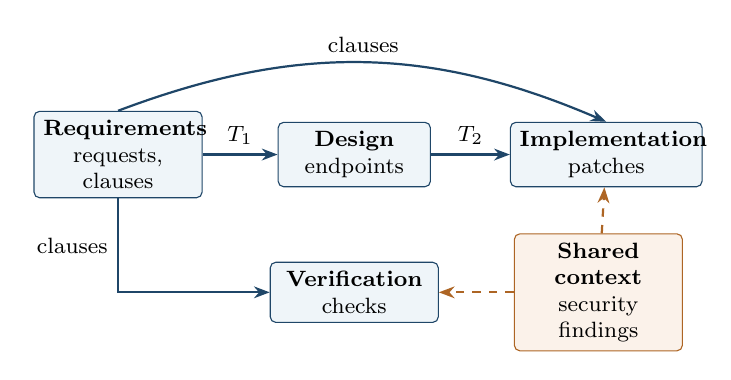
\begin{tikzpicture}[font=\footnotesize]
\node[box,text width=19mm] (r) at (0,0) {\textbf{Requirements}\\requests, clauses};
\node[box,text width=17mm] (d) at (3.0,0) {\textbf{Design}\\endpoints};
\node[box,text width=22mm] (i) at (6.2,0) {\textbf{Implementation}\\patches};
\node[box,text width=19mm] (t) at (3.0,-1.75) {\textbf{Verification}\\checks};
\node[box,text width=19mm,fill=resultamber!10,draw=resultamber!80!black] (c) at (6.1,-1.75) {\textbf{Shared context}\\security findings};
\draw[arr] (r)--node[above]{$T_1$}(d);
\draw[arr] (d)--node[above]{$T_2$}(i);
\draw[arr] (r.south)|-node[pos=0.25,left]{clauses}(t.west);
\draw[arr] (r.north) to[bend left=22] node[above]{clauses}(i.north);
\draw[arr,dashed,draw=resultamber!80!black] (c)--(i);
\draw[arr,dashed,draw=resultamber!80!black] (c)--(t);
\end{tikzpicture}
\caption{Running example. Solid arrows are declared read dependencies; rule $T_1$ derives an endpoint per request and $T_2$ a patch per endpoint. Dashed arrows carry selected shared context. The controller creates objects and references; agents propose only primitive attribute values (signature text, patch body, check oracle).}\label{fig:network}
\end{figure}

The controller, not an agent, decides \emph{which} artifacts exist: one endpoint per accepted request and one patch per endpoint. Agents fill the \emph{slots} inside those artifacts: an endpoint's signature text, a patch body, a check's oracle. We call one such slot a \emph{job}. Fig.~
ef{lst:job} shows the patch job for \texttt{put} in the form the controller stores it; every element is defined in Section~\ref{sec:semantics}, and the walk-through in Section~\ref{sec:walkthrough} follows this job through a change of R02.

\begin{figure}[pos=!htbp]
\centering\footnotesize
\renewcommand{\arraystretch}{1.15}
\begin{tabular}{@{}>{\raggedright\arraybackslash}p{0.215\columnwidth}>{\raggedright\arraybackslash}p{0.725\columnwidth}@{}}
\toprule
Element & Value for the patch job of \texttt{put}\\\midrule
Match key & $q=(\textsf{PatchForEndpoint},\ \texttt{endpoint:put})$\\
Job (slot) & $j=(q,\ \texttt{body})$: the body of the patch for \texttt{put}\\
Target & $\iota(q)=\texttt{patch:put}$, created by the controller\\
Owner & \texttt{coding-agent}\\
Read set $F_j$ & signature of \texttt{endpoint:put}; text of clause R02\\
Observation $o_j$ & \textit{source}: signature \texttt{put(id, body)}; R02 = ``overwriting an archived document returns 409''\newline
\textit{context}: SEC-1 = ``path traversal: reject `/'\,''\newline
\textit{contract}: \texttt{impl-v1}; \textit{owner}: \texttt{coding-agent}\\
Key $\Sig_j$ & $\mathrm{enc}(o_j)$: canonical JSON of $o_j$, compared exactly\\
Request $u$ & $(j,\ e{=}7,\ n{=}1)$; records $\Sig_u=\Sig_j$ and $o_u=o_j$ at dispatch\\
Record $B_j$ & after commit: value $v$, validated key $a=\Sig_u$, committing request $\gamma=u$; \emph{usable} while $a=\Sig_j(S)$ and every prerequisite is usable\\
\bottomrule
\end{tabular}
\caption{One job of the running example as the controller stores it. Editing R02 changes $o_j$ and hence $\Sig_j$, so the stored value becomes unusable although the endpoint signature is unchanged, and a reply to $u$ that arrives after the edit cannot commit. Every element is defined in Section~\ref{sec:semantics}.}\label{lst:job}
\end{figure}

\subsection{Coordination Through Shared Artifacts}\label{sec:bg-mas}
MAS research distinguishes \emph{subjective} coordination, in which agents coordinate by reasoning about each other and exchanging messages, from \emph{objective} coordination, in which a coordination medium outside the agents enforces the rules of interaction~\citep{omicini2001coordination}. Linda introduced a shared tuple space as a coordination medium~\citep{gelernter1985linda,gelernter1992coordination}; tuple centres make the medium's reactions programmable, so that coordination laws are specified once, inside the medium, and apply to every agent~\citep{omicini2001tuple}. The A\&A meta-model generalizes the medium to \emph{artifacts}: passive, typed entities that agents use through operations and that guard their own state~\citep{omicini2008artifacts,weyns2007environment}, as realized in CArtAgO and JaCaMo~\citep{ricci2011environment,boissier2013jacamo}. Interaction protocols specify the admissible message exchanges among autonomous agents. Commitment-based protocols give messages a social meaning that can be checked without inspecting the agents~\citep{singh1998acl,yolum2002commitments}, and information-based protocols such as BSPL derive the admissible orderings from which information each message carries, identified by keys~\citep{singh2011bspl,chopra2020protocols}. Electronic institutions add \emph{governors}: runtime mediators that admit an agent's action only if the institution's current state permits it~\citep{esteva2001institutions,arcos2005institutions,boella2006normative}.

We adopt objective, artifact-mediated coordination. The controller is a coordination artifact: agents can only propose values through one operation (reply to a request), and the artifact's guards decide what becomes visible. Section~\ref{sec:related} details what we inherit and what generative proposals add; in short, the added problems are content currentness of generated values, exact and minimal invalidation, and per-episode budgets.

\subsection{LLM Agents as Untrusted Proposers}\label{sec:bg-agents}
In an LLM framework, each \emph{agent} is a model wrapped with a role instruction and possibly with tools~\citep{metagpt,chatdev,autogen}. The framework sends a prompt assembled from current artifacts and receives text, code or JSON. Three properties of this exchange matter. The reply may be wrong in ways that no prompt prevents~\citep{ji2023hallucination}, and the same prompt may yield different replies. A call takes seconds to minutes, so artifacts may change while it is outstanding. Delivery is unreliable: frameworks time out and retry, so a reply may arrive late, twice or never.

\begin{definition}[Request, proposal, validator, contract]\label{def:proposal}
A \emph{request} is one generation call for one job. It has a unique identity and carries the data the agent may see. A \emph{proposal} is a value returned for a request. A \emph{validator} $V_j$ is a deterministic, total predicate that decides whether a proposal is acceptable for the data it was requested on. The \emph{generation contract} $\eta_j$ of job $j$ identifies everything except data that determines what counts as a correct answer: the instruction, output schema, validator and the environment it runs in (for example, tool versions), generation settings, and the owner allowed to answer. Each request records the contract of its job at dispatch. An agent is an \emph{untrusted proposer}: for safety, we assume nothing about its proposals.
\end{definition}

Changing the contract changes the question, just as changing a requirement does: a reply produced under an old instruction or validator must not be reused as if it answered the new one.

\subsection{Views, Transformations and Traces}\label{sec:bg-views}
Model-driven engineering represents each kind of artifact as a \emph{model} that conforms to a \emph{metamodel}, which makes relations between artifacts explicit.

\begin{definition}[Metamodel, view]\label{def:view}
A \emph{metamodel} declares object types with \emph{primitive attributes} (strings, Booleans, numbers or inert code text), typed \emph{references} with multiplicities, and well-formedness predicates. A \emph{view} is a finite graph conforming to a metamodel. Its nodes are objects with stable identities; its edges are typed references.
\end{definition}

\begin{definition}[Rule, match, trace]\label{def:rule}
A transformation \emph{rule} consists of a source pattern, a guard, one target object type, and \emph{bindings} that compute the target's attributes and references. A \emph{match} is a tuple of source objects that fits the pattern and satisfies the guard; each match yields exactly one target object. A \emph{trace} records which match produced which target~\citep{atl}.
\end{definition}

In the running example, rule $\mathsf{RequestToEndpoint}$ creates one endpoint per accepted request with a reference to it; if the request is deleted, the trace identifies the endpoint to delete. Classical transformations compute every binding with an expression. In our setting some bindings are \emph{generated} by an agent: a job is one generated primitive binding of one target. References are always computed by the controller. Consistency checkers re-evaluate rules after model changes~\citep{egyed2006instant,egyed2011tracking}, and views can be pairwise consistent but jointly inconsistent~\citep{stevens,klare}, so a coordinator also needs a global check before release.

\subsection{Incremental Rebuilding and Optimistic Concurrency}\label{sec:bg-incremental}
After a change, a coordinator must decide which jobs to redo; every redone job costs an LLM call. Build systems face the same choice~\citep{mokhov}. Content-based build systems store a key computed from the contents of a task's dependencies and rebuild the task only if the key changes; with \emph{early cutoff}, a rebuilt task that produces the same output as before does not trigger its dependents~\citep{mokhov,mitchell2012shake}. Dependencies may be dynamic~\citep{erdweg2015pluto}. We use the same idea: the \emph{read set} of a job is the source data its agent may read; together with the selected context and the contract it forms the job's \emph{observation}, whose exact encoding is the job's \emph{dependency key}. One difference remains: an LLM is not a deterministic function, so a regenerated value may differ from the old one although both are valid. A value can therefore be checked only by validating it against the observation it was produced from, never by comparing it with a fresh run.

Locking a job's inputs until its agent answers would block every edit for the duration of an LLM call. Databases solve this with \emph{optimistic concurrency control} (OCC)~\citep{occ}: a transaction computes without locks and, at commit time, validates that the data it read has not changed; validation and write are one atomic step. Our commit guard is such a validation phase: a request records the dependency key of the observation it was dispatched on, and a reply commits only if that key still equals the job's current key.

\subsection{Transition Systems and TLA$^+$}\label{sec:bg-tla}
We specify the controller as a transition system. A \emph{safety property} states that nothing bad happens and is proved with an \emph{invariant}; a \emph{liveness property} states that something good eventually happens. TLA$^+$~\citep{lamport1994tla,lamport2002specifying} specifies such systems; the model checker TLC~\citep{yu1999tlc} explores all states of finite instances, and the proof system TLAPS~\citep{cousineau2012tlaps} checks proofs for all instances. A detailed specification \emph{refines} an abstract one if every behavior of the first, mapped through a refinement mapping, is a behavior of the second~\citep{abadi1991refinement,lynch1995simulations}.

\subsection{Coordination Failures and Requirements}\label{sec:failures}\label{sec:requirements}
The running example admits four failure classes that per-answer checks cannot exclude:
\begin{itemize}
\item[\textbf{F1}] \emph{Stale reply.} A request is sent while R02 has revision~1, R02 changes, and the old reply then arrives. It is well formed and may pass the old tests.
\item[\textbf{F2}] \emph{Local validity, global inconsistency.} Design chooses string identifiers and verification integer identifiers. Both pass their local validators.
\item[\textbf{F3}] \emph{Unsafe change of team or rules.} A reviewer is added, a permission is revoked, or a prompt or validator changes, and old evidence or old completion verdicts are reused as if nothing had changed.
\item[\textbf{F4}] \emph{Unbounded or wasted generation.} A failing request is retried on every scheduler pass, or an unrelated edit regenerates every artifact.
\end{itemize}
A coordinator for untrusted generative agents should therefore satisfy six requirements; Section~\ref{sec:guarantees} answers each with a theorem.
\begin{itemize}
\item[\textbf{R1}] \emph{Structural integrity.} Objects, traces and references are well typed and have exactly one producer, whatever the agents return.
\item[\textbf{R2}] \emph{Currentness.} A value is usable only if it was validated against the \emph{current} observation, contract and owner; obsolete and duplicate replies cannot write (F1, F3).
\item[\textbf{R3}] \emph{Honest completion.} Publication requires that nothing is pending or stale and that all joint constraints hold (F2, F3).
\item[\textbf{R4}] \emph{Locality.} A change invalidates exactly the work whose observations changed (F4).
\item[\textbf{R5}] \emph{Bounded effort and termination.} Generation attempts are bounded, and a stable workflow ends with an explicit success or failure verdict (F4).
\item[\textbf{R6}] \emph{Safe reconfiguration.} Changing agents, rules, permissions or validators preserves R1--R3 (F3).
\end{itemize}

\begin{table}[pos=!htbp]
\centering
\caption{Terms used in this paper, their symbols, and their standard counterparts in MAS coordination, databases and build systems. Formal definitions are in Section~\ref{sec:semantics}.}\label{tab:glossary}
\footnotesize\setlength{\tabcolsep}{3pt}
\begin{tabular}{@{}P{20mm}P{13mm}P{61mm}P{56mm}@{}}\toprule
Term & Symbol & Meaning in this paper & Standard counterpart\\\midrule
Controller & -- & Deterministic component that owns structure, keys, acceptance and publication & Coordination artifact (A\&A); tuple centre; institutional governor\\
Job (slot) & $j=(q,b)$ & One generated primitive attribute $b$ of the target of match $q$ & Build task; artifact operation with one output\\
Read set & $F_j$ & Source data the job's agent may read (a pure query, including membership) & Read set of a transaction; declared/dynamic build dependencies\\
Contract & $\eta_j$ & Instruction, schema, validator and its environment, generation settings, owner & Build rule plus toolchain version; protocol role\\
Observation & $o_j$ & Read set, selected context and contract: all the job depends on & Materialized read set plus task configuration\\
Dependency key & $\Sig_j$ & Exact injective encoding $\operatorname{enc}(o_j)$ & Content-addressed rebuild key (verifying trace)\\
Validated key & $a_j$ & The key against which the stored value was validated & Read-set version validated at OCC commit\\
Episode & $e_j$, $n_j$ & Maximal period in which a job keeps one key; attempt counter $n_j\le k$ & Invalidation epoch with a retry budget\\
Request & $u=(j,e,n)$ & One generation call; identity never reused & Message identifier / BSPL key; transaction identifier\\
Accepted / usable & $U_j$ & Accepted: a value was once validly committed. Usable: its validated key is current and all prerequisites are usable & Committed vs.\ current version; up-to-date build target\\
Publishable & $\mathit{Pub}$ & Nothing suspended, stale or pending; global predicate $G$ holds (Eq.~\eqref{eq:publish}, written $\Pub(S)$) & Release gate; institutional completion condition\\
Suspended stage & $Q$ & Stage whose prerequisites are unavailable; contributes no jobs & Blocked task; disabled scene in an institution\\\bottomrule
\end{tabular}
\end{table}


% =====================================================================
\section{Approach Overview}\label{sec:overview}

\subsection{Design Principles and Their Lineage}
The approach rests on four principles. Each refines an established idea for the setting of generated artifacts.
\begin{enumerate}
\item \emph{Agents propose, the controller disposes.} Agents never create objects, references or completion verdicts; they return a primitive value for a slot that the controller created. This is objective coordination through an artifact~\citep{omicini2001tuple,omicini2008artifacts}: the coordination laws live in the controller, not in the agents' prompts.
\item \emph{Depend on exactly what was observed.} Each request is rendered from an explicit observation: the read set, selected context and contract. Its exact encoding is the job's dependency key, as in content-addressed build systems~\citep{mokhov}. Because the agent sees nothing else, its input dependencies are exact by construction; what remains to be shown for correctness is that the validator judges the right relation (Definition~\ref{def:adequate}).
\item \emph{Commit atomically and only if current.} The check ``is this reply still the answer to the current question?'' and the write form one transaction, as in OCC~\citep{occ}. Like an institutional governor~\citep{esteva2001institutions}, the controller judges an action in the current state, not in the state in which it was requested.
\item \emph{Separate accepted, usable and publishable.} A value accepted earlier may become outdated after an edit. It remains as history, but consumers read only \emph{usable} values, and release happens only through a global \emph{publication barrier}.
\end{enumerate}

\subsection{Who Specifies What}\label{sec:roles}
A recurring concern with formally grounded coordination is that someone must write the specifications. Table~\ref{tab:roles} separates the roles. The TLA$^+$ model, its refinement mapping and the proofs concern the \emph{generic} protocol. Framework builders write and check them once, as they would for any concurrency-control algorithm. A workflow author never writes TLA$^+$. They declare jobs in ordinary code: stage, prerequisites, owner, read-set function, context selector, contract and validator. The controller derives structure, keys, episodes and publication from these declarations. For the two LLM studies of Section~\ref{sec:evaluation}, the complete workflow declarations take \WorkflowDeclLines{} and \BenchDeclLines{} lines of Python, and their validators \WorkflowValidatorLines{} lines plus a \SandboxLines-line sandboxed property checker. The cost of a workflow therefore lies in its validators, which a team that tests its software already writes. The coordination guarantees do not depend on how strong those validators are. The correctness of the released artifacts does (Corollary~\ref{cor:domain}), and RQ6 measures that gap on standard benchmarks.

\begin{table}[pos=!htbp]
\centering
\caption{Division of labor. Only the first row involves formal methods, and it is independent of any particular workflow.}\label{tab:roles}
\footnotesize\setlength{\tabcolsep}{3pt}
\begin{tabular}{@{}P{17mm}P{39mm}P{25mm}@{}}\toprule
Role & Writes & In this paper\\\midrule
Framework builder (once) & Controller kernel; TLA$^+$ model, refinement mapping, proofs & \texttt{src/vgc} (\GraphLines{} lines for the generic kernel); \TLALines{} lines of TLA$^+$\\
Workflow author (per workflow) & Jobs: stage, prerequisites, owner, read set, context selector, contract, validator; global predicate $G$ & \WorkflowDeclLines{} + \WorkflowValidatorLines{} lines (RQ5); \BenchDeclLines{} lines (RQ6)\\
Editors, administrators & Inputs, context, configuration changes & Change streams\\
Agents & Primitive values only & LLMs or scripts\\\bottomrule
\end{tabular}
\end{table}

\begin{figure}[pos=!htbp]
\centering
\colorlet{inkblue}{black}\colorlet{pale}{gray!12}\colorlet{resultamber}{gray}% grayscale figure
\resizebox{\textwidth}{!}{%
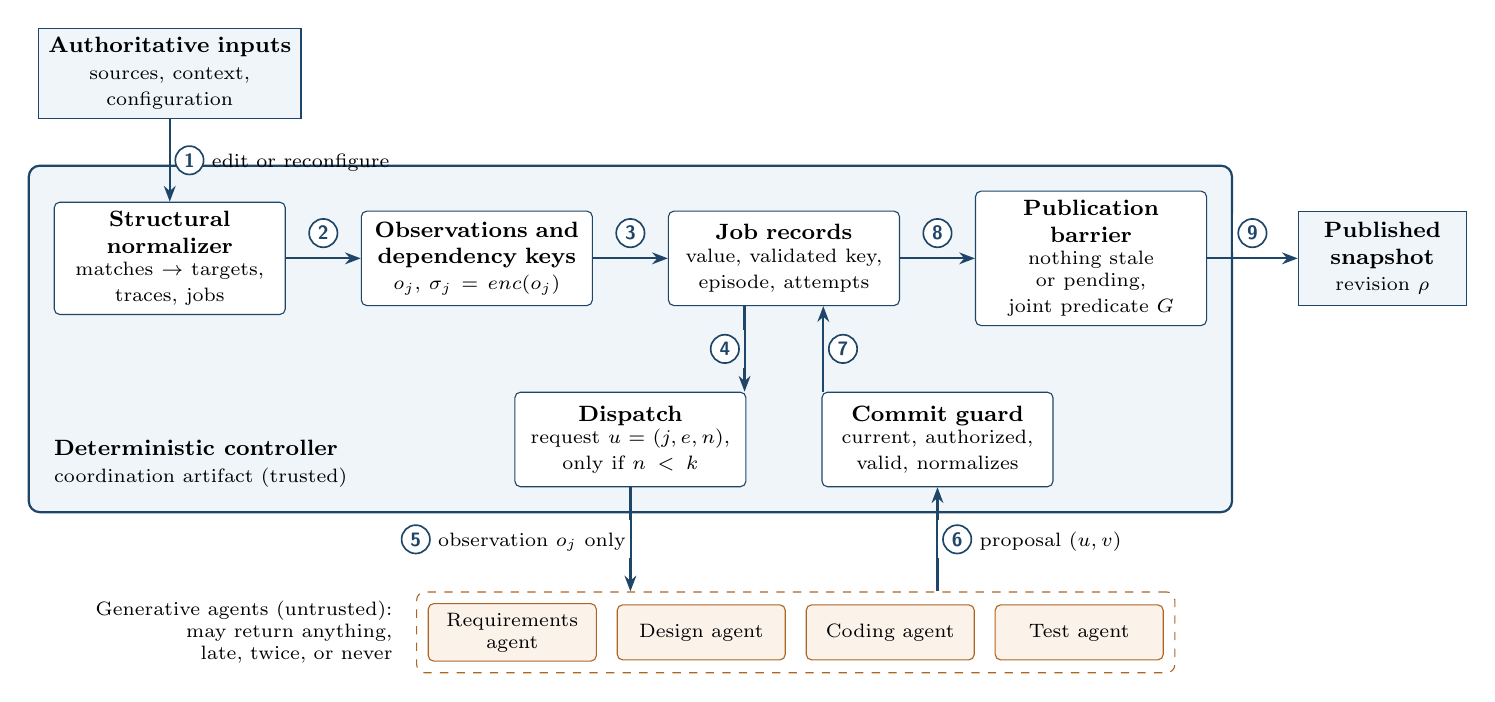
\begin{tikzpicture}[font=\footnotesize,
  comp/.style={draw=inkblue,rounded corners=2pt,fill=white,align=center,minimum height=12mm,text width=27mm},
  agent/.style={draw=resultamber!80!black,fill=resultamber!10,rounded corners=2pt,align=center,text width=19mm,minimum height=7mm,font=\scriptsize},
  lab/.style={font=\scriptsize,align=left,inner sep=1.5pt,fill=pale}]
% row 1: structure and records
\node[comp] (norm) at (0,0) {\textbf{Structural normalizer}\\\scriptsize matches $\to$ targets,\\traces, jobs};
\node[comp] (obs)  at (3.9,0) {\textbf{Observations and}\\\textbf{dependency keys}\\\scriptsize $o_j$, $\Sig_j=\operatorname{enc}(o_j)$};
\node[comp] (rec)  at (7.8,0) {\textbf{Job records}\\\scriptsize value, validated key,\\episode, attempts};
\node[comp] (pub)  at (11.7,0) {\textbf{Publication barrier}\\\scriptsize nothing stale or pending,\\joint predicate $G$};
% row 2: interaction with agents
\node[comp] (disp)  at (5.85,-2.3) {\textbf{Dispatch}\\\scriptsize request $u=(j,e,n)$,\\only if $n<k$};
\node[comp] (guard) at (9.75,-2.3) {\textbf{Commit guard}\\\scriptsize current, authorized,\\valid, normalizes};
% controller boundary
\begin{scope}[on background layer]
\node[draw=inkblue,thick,rounded corners=4pt,fill=pale,fit=(norm)(pub)(disp)(guard),inner xsep=9pt,inner ysep=9pt] (ctrl) {};
\end{scope}
\node[anchor=south west,font=\footnotesize\bfseries,align=left] at ([xshift=6pt,yshift=6pt]ctrl.south west) {Deterministic controller\\\normalfont\scriptsize coordination artifact (trusted)};
% outside
\node[draw=inkblue,fill=pale,align=center,text width=31mm,minimum height=9mm] (inp) at (0,2.35) {\textbf{Authoritative inputs}\\\scriptsize sources, context, configuration};
\node[draw=inkblue,fill=pale,align=center,text width=19mm,minimum height=12mm] (snap) at (15.4,0) {\textbf{Published}\\\textbf{snapshot}\\\scriptsize revision $\rho$};
\node[agent] (a1) at (4.35,-4.75) {Requirements agent};
\node[agent] (a2) at (6.75,-4.75) {Design agent};
\node[agent] (a3) at (9.15,-4.75) {Coding agent};
\node[agent] (a4) at (11.55,-4.75) {Test agent};
\begin{scope}[on background layer]
\node[draw=resultamber!80!black,dashed,rounded corners=3pt,fit=(a1)(a4),inner sep=4pt] (agents) {};
\end{scope}
\node[anchor=east,font=\scriptsize,align=right] at ([xshift=-5pt]agents.west) {Generative agents (untrusted):\\may return anything,\\late, twice, or never};
% numbered flow
\draw[arr] (inp) -- node[lab,right,fill=none]{\step{1} edit or reconfigure} (norm);
\draw[arr] (norm) -- node[lab,above=2pt]{\step{2}} (obs);
\draw[arr] (obs) -- node[lab,above=2pt]{\step{3}} (rec);
\draw[arr] (rec.south) ++(-0.5,0) coordinate (r1) -- (r1 |- disp.north) node[lab,midway,left]{\step{4}};
\draw[arr] (disp.south) -- node[lab,left,fill=white]{\step{5} observation $o_j$ only} (disp.south |- agents.north);
\draw[arr] (guard.south |- agents.north) -- node[lab,right,fill=white]{\step{6} proposal $(u,v)$} (guard.south);
\draw[arr] (guard.north) ++(-1.45,0) coordinate (g1) -- (g1 |- rec.south) node[lab,midway,right]{\step{7}};
\draw[arr] (rec) -- node[lab,above=2pt]{\step{8}} (pub);
\draw[arr] (pub) -- node[lab,above=2pt,fill=white]{\step{9}} (snap);
\end{tikzpicture}}
\caption{Architecture. Agents (bottom) receive only a declared observation and return a primitive proposal. Structure, dependency keys, attempt budgets, acceptance and publication belong to the controller. The numbered steps are explained in Section~\ref{sec:walkthrough}.}\label{fig:overview}
\end{figure}

\subsection{Walk-Through of One Change}\label{sec:walkthrough}
Fig.~\ref{fig:overview} shows the architecture. We follow the tightened R02 clause and the patch job of Fig.~\ref{lst:job} through it; Fig.~\ref{fig:sequence} shows the same run as a message sequence, including a stale reply.
\begin{steps}
\item[\step{1}] An authorized editor changes R02. Every input change and every configuration change is one atomic controller transaction.
\item[\step{2}] The \emph{structural normalizer} recomputes the matches of $T_1$ and $T_2$ and creates or deletes targets and traces. Here no object changes, because the request still exists.
\item[\step{3}] For each job the controller recomputes the observation. The patch job's observation contains the clause text, so its key changes; jobs of unrelated requests keep their keys and their values remain usable.
\item[\step{4}] A job whose key changed starts a new \emph{episode} with a fresh attempt budget, and any request still in flight for the old episode is cancelled. Jobs whose prerequisites are unusable are suspended, not dispatched.
\item[\step{5}] The controller dispatches a request with a fresh identity $u=(j,e,n)$; the prompt is rendered from $o_j$ only.
\item[\step{6}] The agent returns a proposal, perhaps late, perhaps twice, perhaps malformed.
\item[\step{7}] The \emph{commit guard} checks atomically that $u$ is still active, that its recorded key equals the job's current key, that the owner is still authorized, that the validator accepts the value, and that the resulting structure normalizes. Only then does the value become \emph{usable}. The stale reply in Fig.~\ref{fig:sequence} fails the first two checks and is discarded.
\item[\step{8}] The \emph{publication barrier} releases a snapshot only if no required stage is suspended, no job is stale or pending, and the global predicate $G$ holds; for example, $G$ requires design and verification to agree on the identifier type (F2). Publication \step{9} installs the snapshot with its revision.
\end{steps}

\begin{figure}[pos=!htbp]
\centering
\colorlet{inkblue}{black}\colorlet{pale}{gray!12}\colorlet{resultamber}{gray}% grayscale figure
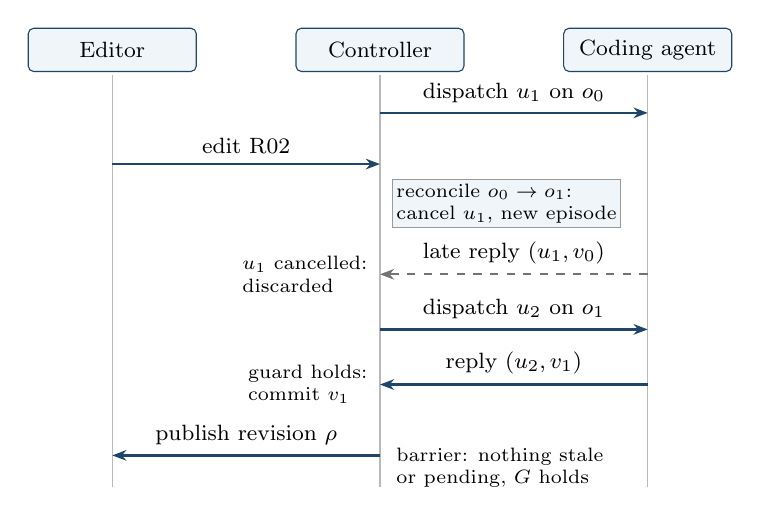
\begin{tikzpicture}[font=\footnotesize,
  msg/.style={-{Stealth[length=1.8mm]},thick,draw=inkblue},
  bad/.style={-{Stealth[length=1.8mm]},thick,draw=black!55,dashed},
  note/.style={font=\scriptsize,align=left,fill=white,inner sep=1.5pt}]
\foreach \x/\n in {0/Editor,3.4/Controller,6.8/Coding agent} {
  \node[box,text width=19mm,minimum height=5.5mm] at (\x,0) {\n};
  \draw[gray!55] (\x,-0.32) -- (\x,-5.55);}
\draw[msg] (3.4,-0.8) -- node[above]{dispatch $u_1$ on $o_0$} (6.8,-0.8);
\draw[msg] (0,-1.45) -- node[above]{edit R02} (3.4,-1.45);
\node[note,anchor=west,draw=black!40,fill=pale] at (3.55,-1.95) {reconcile $o_0\to o_1$:\\cancel $u_1$, new episode};
\draw[bad] (6.8,-2.85) -- node[above]{late reply $(u_1,v_0)$} (3.4,-2.85);
\node[note,anchor=east] at (3.3,-2.85) {$u_1$ cancelled:\\discarded};
\draw[msg] (3.4,-3.55) -- node[above]{dispatch $u_2$ on $o_1$} (6.8,-3.55);
\draw[msg] (6.8,-4.25) -- node[above]{reply $(u_2,v_1)$} (3.4,-4.25);
\node[note,anchor=east] at (3.3,-4.25) {guard holds:\\commit $v_1$};
\draw[msg] (3.4,-5.15) -- node[above]{publish revision $\rho$} (0,-5.15);
\node[note,anchor=north west] at (3.55,-5.0) {barrier: nothing stale\\or pending, $G$ holds};
\end{tikzpicture}
\caption{Failure F1 handled by the controller. The edit cancels $u_1$; its late reply cannot commit even if it passes the old validator. If R02 later reverts to $o_0$, a new episode starts and $u_1$ remains cancelled. RQ5 measures this situation with real LLMs.}\label{fig:sequence}
\end{figure}


% =====================================================================
\section{Formal Semantics}\label{sec:semantics}
We model the controller as a labeled transition system $(\mathcal S,\mathcal S_0,\Lambda,\to)$ with states $\mathcal S$, initial states $\mathcal S_0$, event labels $\Lambda$ and a transition relation. Keys, identities and primitive values are unbounded, so the system is infinite-state; diagrams such as Fig.~\ref{fig:automaton} are automaton \emph{schemas}. For safety, the proposal source is fully nondeterministic: it may return any value, malformed data, duplicates, or nothing. This over-approximates every LLM behavior without probabilistic assumptions. The section builds the semantics bottom-up: the structural kernel that decides which artifacts exist, including deferred structural checks (Section~\ref{sec:deferred}), observations and keys, the controller state, the reconciliation operator that recomputes keys after a change, the transition rules, and finally the assumptions on which the guarantees of Section~\ref{sec:guarantees} rest.

\subsection{Views, Rules and the Structural Kernel}
Views and metamodels are as in Definition~\ref{def:view}. Let $X$ denote the authoritative source views together with immutable shared-context snapshots. Collection membership, object existence and the absence of a context item are observable data: a dependency analysis that looked only at existing attribute values would miss additions and deletions.

A configuration $C$ contains view metamodels, transformation rules, ownership, context-selection policies, validators, generation contracts and a global predicate $G$. Reads are \emph{ranked} (assumption A0 in Table~\ref{tab:assumptions}): rule matches, structural expressions, observations, selectors and validators read only external data or strictly earlier stages. A \emph{stage} groups independent rules processed after their prerequisites.

A rule has a tuple source pattern, a deterministic guard, one target object, deterministic structural bindings, and zero or more generated primitive bindings. A match is identified by the key $q=(r,\operatorname{id}(s_1),\ldots,\operatorname{id}(s_m))$, for example $(\mathsf{RequestToEndpoint},\ \mathsf{request17})$. A deterministic injective constructor yields the target identity $\iota(q)$ and the persistent trace $q\mapsto\iota(q)$. Producers use disjoint identifier namespaces. A reference resolves through traces only if the referenced match exists; a missing mandatory target makes normalization fail instead of leaving a dangling reference.

The \emph{structural normalizer} $N_C$ maps a coherent snapshot to a skeleton: it computes the current match set, creates missing targets, removes obsolete targets and their traces, and computes deterministic attributes and references. Generated slots without a value hold $\nodata$. $N_C$ is partial: inadmissible candidates are rejected.

\begin{definition}[Structural admissibility]\label{def:struct}
Configuration $C$ is \emph{structurally admissible} on a snapshot if $N_C$ terminates, is deterministic and idempotent, produces exactly one owned target and trace per match key, creates only well-typed references, and satisfies all multiplicity constraints. Generated bindings write only declared primitive slots, and every write has exactly one configured owner.
\end{definition}

\begin{theorem}[Constructive structural kernel]\label{thm:kernel}
Consider finite source graphs and finitely many single-target rules whose guards and structural expressions are pure and terminating. Suppose target identities $\iota(q)$ are injective, producer namespaces are disjoint, primitive expressions have declared types, and each reference expression returns a finite set of current match keys of the required target type and multiplicity. Then enumerating matches, allocating all targets, and resolving references constructs an admissible skeleton. The result is unique, and idempotent when generated slots are held fixed.
\end{theorem}
\begin{proof}
Each source product is finite, so terminating guards yield a finite match set. Allocation creates one target per key; injectivity and disjoint namespaces exclude collisions, and the trace is exactly the graph of $\iota$ on that set. Each reference key lies in this domain by hypothesis, so second-phase lookup succeeds and preserves type and cardinality. Typed primitive expressions preserve attribute types. Purity makes the match set and structural values independent of enumeration order, which gives uniqueness, and repeating the construction yields the same keys, identities, references and values, which gives idempotence. Deleting targets outside the current key set yields exact coverage. Induction over the finite rank order extends the argument to all enabled stages.
\end{proof}

If a prerequisite stage is unavailable, its dependent stage is \emph{suspended}: it contributes no active targets, traces or jobs, and a set $Q$ records suspended required stages so that an empty job set is never mistaken for completion. Retained records of a suspended job cannot be read by consumers; on reactivation, stable keys reconstruct the objects and a retained value becomes usable only by the restore rule of Section~\ref{sec:recon}.

\subsection{Deferred Structural Checks}\label{sec:deferred}
A generated attribute may be read by a structural expression of a later stage. In the case study, the architecture's identifier type feeds the implementation's identity expression, which requires strings. A natural design evaluates such expressions only for \emph{enabled} consumers. A locally valid integer identifier committed while the implementation stage is suspended is then admissible, and every later reactivation of the implementation stage fails normalization and is refused, until someone changes the architecture value. Safety is preserved, but the workflow cannot make progress: a liveness hazard and a gap in the terminal-outcome argument. Our semantics removes it in two complementary ways.
\begin{itemize}
\item[\textbf{(a)}] \emph{Configured-consumer checks.} The commit guard evaluates, on the candidate, every structural expression of every \emph{configured} consumer that reads the slot, whether or not the consumer is currently enabled (assumption A1).
\item[\textbf{(b)}] \emph{Invalidate, do not refuse.} If an input edit or reconfiguration makes a structural expression fail because of an already-committed generated value, the transaction does not reject the edit. It demotes that value to history, so its job becomes stale and is regenerated, and normalization is retried. Only failures caused by the inputs themselves reject the edit.
\end{itemize}
Rule (b) terminates because each retry removes one generated value and there are finitely many. In the case study, structural expressions read only generated values, so (a) suffices and (b) never fires. RQ1 measures the hazard under the enabled-only semantics: \EnabledOnlyRefusals{} authorized changes were refused in \EnabledOnlyRuns{} of \AblRuns{} randomized executions, and none under our semantics.

\subsection{Observations and Dependency Keys}
A job $j=(q,b)$ is one generated attribute $b$ of the target of match $q$. Let $Z$ be the coherent readable snapshot formed from $X$ and the currently usable generated predecessors, built in rank order. The job's \emph{observation} is
\begin{equation}\label{eq:obs}
o_j=\obs_{C,j}(Z)=\bigl(F_j(Z),\ \operatorname{select}_{C,j}(Z),\ \eta_{C,j}\bigr),
\end{equation}
where $F_j$ is a pure, total read-set expression, $\operatorname{select}_{C,j}$ returns the authorized context items (including explicit absence markers), and $\eta_{C,j}$ is the generation contract of Definition~\ref{def:proposal}: instruction, schema, validator and its environment, read-set expression, selection policy, generation settings and the \emph{owner} $\omega_{C,j}$. Because the owner is part of $\eta$, revoking or reassigning ownership changes the key of every affected job. A configuration change need not invalidate every job, but it must change $\eta$ for every job it affects. We write $o_j$, $\eta_j$ when $C$ is clear.

The \emph{dependency key} $\Sig_j=\operatorname{enc}(o_j)$ is an injective canonical encoding: different observations never share an encoding. An implementation may store the encoding or a digest with collision detection; a bare cryptographic digest makes the results conditional on the absence of collisions. Context version numbers enter $o_j$ only if the agent or validator actually sees them; otherwise equal selected content at different versions has equal keys (scenario S10).

A read set describes a dependency \emph{function}, not merely the locations visited last time: the query ``all findings for endpoint $e$'' depends on the membership of that set as well as on its contents, so adding a matching finding changes the observation (scenario S09). Unavailable or access-denied context yields $o_j=\nodata$ and blocks dispatch; silently substituting empty text would change the question.

\begin{definition}[Read-set adequacy, validator soundness]\label{def:adequate}
Let $R_j(Z,v)$ be the desired domain relation between snapshots and proposed values. A read set is \emph{adequate} for $R_j$ if there is $\widehat R_j$ with $R_j(Z,v)=\widehat R_j(o_j,v)$ for all admissible $Z,v$. A validator $V_j(o,v)$ is \emph{sound} for $R_j$ if $V_j(o,v)\Rightarrow\widehat R_j(o,v)$.
\end{definition}

Two snapshots with the same observation must yield the same validity judgment for any proposal. Because prompts are rendered from $o_j$ only, the agent's own input dependency is exact by construction; adequacy is a property of the \emph{desired relation}. A read set containing only the endpoint signature is not adequate for R02, because two snapshots may have equal signatures and different clauses. No freshness mechanism can repair an inadequate read set.

\subsection{Controller State}
Table~\ref{tab:state} lists the components of the state $S=(C,X,Y,L,B,P,A,H,Q,\nu,\rho)$ with their types. The first group is operational state that guards read; the second is append-only audit state that only the request-uniqueness guard and the publication record read. For each job $j$, $B_j$ is its record. It holds an accepted triple $(v,a,\gamma)$ of value, validated key and evidence (the committing request) or none; a failure mark $f$; an episode nonce $e$ with the episode key $s$; and an attempt counter $n\in\{0,\ldots,k\}$ for a fixed budget $k\ge1$.

\begin{table}[pos=!htbp]
\centering
\caption{Controller state. $\mathsf{Key}$ is the set of encoded observations; $\mathsf{Id}$ request identities; $\mathsf{Val}$ primitive values.}\label{tab:state}
\footnotesize\setlength{\tabcolsep}{3pt}
\begin{tabular}{@{}lP{33mm}P{36mm}@{}}\toprule
& Type & Role\\\midrule
$C$ & configuration & rules, owners, contracts, validators, $G$\\
$X$ & source views $\times$ context snapshots & authoritative inputs\\
$Y$ & typed graph & active skeleton (targets, references)\\
$L$ & $\mathsf{MatchKey}\rightharpoonup\mathsf{TargetId}$ & traces\\
$B$ & $\Jobs\rightharpoonup\mathsf{Record}$ & job records $B_j=(\mathit{acc},f,e,s,n)$, $\mathit{acc}\in\{(v,a,\gamma),\bot\}$\\
$P$ & $\mathsf{Id}\rightharpoonup\mathsf{Req}$, $\mathsf{Req}=\Jobs\times\mathbb N\times\mathsf{Key}\times\mathsf{Obs}\times\mathsf{Owner}$ & active requests\\
$Q$ & set of stages & suspended required stages\\\midrule
$A$ & $\mathsf{Id}\rightharpoonup\mathsf{Req}$ (append-only) & every dispatched request\\
$H$ & snapshot $\times$ revision, or none & last publication\\
$\nu$ & $\mathbb N$ & monotone nonce allocator\\
$\rho$ & $\mathbb N$ & semantic revision counter\\\bottomrule
\end{tabular}
\end{table}

For an active job, freshness, usability and the set of outstanding obligations are defined in rank order:
\begin{align}
\fresh_j(S)&\iff B_j.\mathit{acc}=(v,a,\gamma)\ \land\ a=\Sig_j(S),\label{eq:fresh}\\
U_j(S)&\iff j\text{ active}\land\fresh_j(S)\land\textstyle\bigwedge_{i\prec j}U_i(S),\label{eq:usable}\\
O(S)&=\{j\in\Jobs(S):\neg U_j(S)\}.\label{eq:obligation}
\end{align}
Here $i\prec j$ ranges over declared generated prerequisites. Consumers read a value only through the $U_j$ gate: if an upstream value becomes unusable, all its descendants become unusable too. Validators are total and deterministic on their declared observations; validators that call external tools include tool versions in the contract.

\subsection{Reconciliation}\label{sec:recon}
After every committed input edit, reconfiguration or acceptance, the controller applies the reconciliation operator $\mathcal R$ to the candidate state. Stage by stage in rank order, $\mathcal R$ normalizes the stage with $N_C$, recomputes $Q$, and for every active job $j$ with new key $\Sig'_j=\Sig_j(S')$:
\begin{equation}\label{eq:recon}
\begin{aligned}
B'_j&=B_j &&\text{if } j \text{ was active and } s_j=\Sig'_j,\\
B'_j&=(B_j.\mathit{acc},\bot,\nu{+}1,\Sig'_j,0) &&\text{otherwise (new episode)},
\end{aligned}
\end{equation}
allocating a fresh nonce from $\nu$ for each new episode. It then cancels every request in $P$ whose job is inactive or whose episode, key or owner no longer matches. A new episode keeps the accepted triple as \emph{retained evidence}. By~\eqref{eq:fresh}, the retained value becomes usable again immediately if and only if its validated key equals the new key, for example when an upstream job is repaired to the same value (early cutoff) or a job is reactivated with an unchanged observation. Retaining one triple per job is a one-entry cache. A multi-entry memo table indexed by key, as in Shake~\citep{mitchell2012shake}, would also restore values after reversions such as $o_0\to o_1\to o_0$, but we do not assume one.

Candidate states are private: if a candidate is discarded, everything it allocated is discarded with it, including nonces. A nonce is exposed only when a request carrying it is dispatched from a committed state, and $A$ retains every dispatched request, so request identities are never reused across committed states, even after deletion and recreation of a job.

Fig.~\ref{fig:automaton} summarizes a job's control states, which are derived from its record. A dependency change cancels pending authority and starts a new episode; the job is then Dirty, unless its retained evidence matches the new key, in which case it is immediately Fresh. Failed is terminal for an unchanged episode but is not a successful state. No agent can move a job to Fresh directly.

\begin{figure}[pos=!htbp]
\centering
\colorlet{inkblue}{black}\colorlet{pale}{gray!12}%
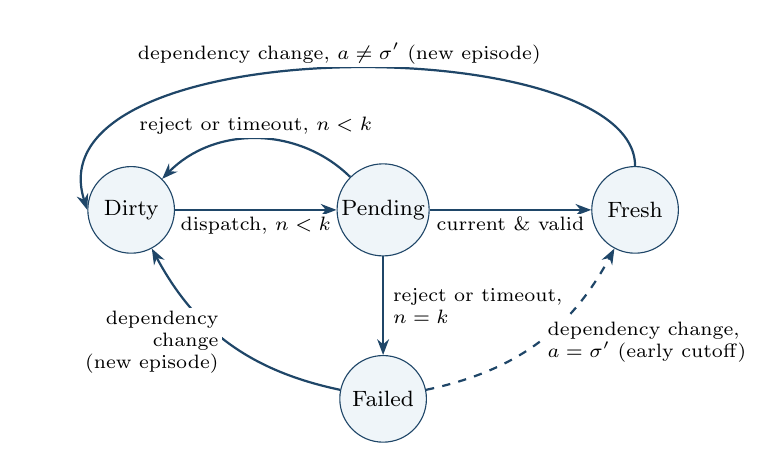
\begin{tikzpicture}[>=Stealth,every state/.style={draw=inkblue,fill=pale,font=\footnotesize,minimum size=11mm,inner sep=1pt},
  lab/.style={font=\scriptsize,fill=white,inner sep=1.2pt}]
\node[state] (d) at (0,0) {Dirty};
\node[state] (p) at (3.2,0) {Pending};
\node[state] (f) at (6.4,0) {Fresh};
\node[state] (e) at (3.2,-2.4) {Failed};
% forward path
\draw[arr] (d) -- node[lab,below=1pt]{dispatch, $n<k$} (p);
\draw[arr] (p) -- node[lab,below=1pt]{current \& valid} (f);
% retry
\draw[arr] (p) to[bend right=45] node[lab,above]{reject or timeout, $n<k$} (d);
% budget exhausted
\draw[arr] (p) -- node[lab,right=2pt,align=left]{reject or timeout,\\$n=k$} (e);
% dependency changes
\draw[arr] (f.north) .. controls (6.4,2.3) and (-1.3,2.3) .. node[lab,above,pos=0.5]{dependency change, $a\neq\Sig'$ (new episode)} (d.west);
\draw[arr] (e) to[bend left=25] node[lab,left=2pt,align=right]{dependency\\change\\(new episode)} (d);
\draw[arr,dashed] (e) to[bend right=25] node[lab,right=2pt,align=left]{dependency change,\\$a=\Sig'$ (early cutoff)} (f);
\end{tikzpicture}
\caption{Control automaton schema of one job. Solid arrows are controller transitions; the dashed arrow is early cutoff. A dependency change always starts a new episode and cancels pending requests; if the retained evidence's validated key $a$ equals the new key $\Sig'$, the job becomes Fresh at once, from any state and without a request. Obsolete replies never cause a transition, and no agent can move a job to Fresh.}\label{fig:automaton}
\end{figure}

\subsection{Transition Rules}\label{sec:rules}
Every transition is one atomic controller transaction; Table~\ref{tab:rules} lists them. Two rules deserve comment.

\emph{Resolve.} For a returned pair $(u,v)$, let $\Sig_u$ and $o_u$ be the key and observation recorded in request $u$. The commit guard requires that $u$ is active in $P$ and belongs to the job's current episode, that its owner is still authorized, that all prerequisites are usable, that $v$ has the slot's primitive type, and that
\begin{equation}\label{eq:guard}
\Sig_u=\Sig_j(S),\qquad o_j(S)\ne\nodata,\qquad V_j(o_u,v).
\end{equation}
The value is first installed in a private \emph{candidate} state, on which $\mathcal R$ and the configured-consumer structural checks of Section~\ref{sec:deferred} run. The candidate is committed only if they succeed; otherwise the attempt counts as rejected. The equality test and the write share one linearization point~\citep{herlihy1990linearizability} with edits and reconfigurations. Validation may run outside the transaction on the immutable $o_u$; the reference controllers do exactly that, and the result counts only after the guard is rechecked inside the transaction. This is OCC~\citep{occ}.

\emph{Publish.} Let $G$ be a total predicate over an immutable candidate snapshot that encodes all joint constraints and required executable checks. Then
\begin{equation}\label{eq:publish}
\begin{split}\Pub(S)\iff{}&\text{normal form}\land Q=\emptyset\land O(S)=\emptyset\\&{}\land P=\emptyset\land G(C,X,Y,B,L).\end{split}
\end{equation}
Only a Publish transition satisfying~\eqref{eq:publish} installs $H$ with that exact snapshot and revision. Later edits leave $H$ as a historical snapshot and remove any claim that it is current.

\begin{remark}[Redundancy of $P=\emptyset$]\label{rem:pending}
With cancellation, every request in $P$ belongs to a job in the current episode that has not yet committed, so $P\neq\emptyset$ implies $O(S)\neq\emptyset$ in reachable states. The conjunct $P=\emptyset$ in~\eqref{eq:publish} is therefore implied, and the abstract machine of Section~\ref{sec:refinement} can omit it. We keep it as a defense that remains valid if cancellation is disabled.
\end{remark}

\begin{table}[pos=!htbp]
\centering
\caption{Controller transitions and their counterparts in the atomic specification used for refinement (Theorem~\ref{thm:refinement}). Unmentioned components are unchanged; $\mathcal R$ is reconciliation, Eq.~\eqref{eq:recon}.}\label{tab:rules}
\footnotesize\setlength{\tabcolsep}{4pt}
\begin{tabular}{@{}P{20mm}P{57mm}P{52mm}P{19mm}@{}}\toprule
Transition & Guard & Effect & Abstract action\\\midrule
Edit / Normalize & Authorized edit; candidate passes $N_C$ (after rule (b) of Sec.~\ref{sec:deferred}) & Install input; apply $\mathcal R$; advance $\rho$. If the inputs themselves are inadmissible, keep the state and record a rejection & Edit\\
Dispatch$(j)$ & $j\in O(S)$; $o_j\ne\nodata$; prerequisites usable; no active request for $j$; $f\ne\Sig_j$; $n<k$ & $n\gets n+1$; record request $u=(j,e,n)$ with $(\Sig_j,o_j,\omega_j)$ in $P$ and $A$; send only $o_j$ & Attempt\\
Resolve (commit) & $u\in P$; current episode; owner authorized; Eq.~\eqref{eq:guard}; type check; candidate normalizes for all configured consumers & Install $(v,\Sig_u,u)$; clear $f$; remove $u$; apply $\mathcal R$; advance $\rho$ & Accept\\
Resolve (reject) / Timeout & $u\in P$ current, but validation, typing or normalization fails, or timeout & Remove $u$; if $n=k$ set $f\gets\Sig_j$ & Fail\\
Discard & $u\notin P$, obsolete or unauthorized & None (duplicate or late delivery) & Stutter\\
Publish & Eq.~\eqref{eq:publish} on an immutable snapshot & Install $H$ with that snapshot and revision & Publish\\
Reconfigure & Candidate $C'$ admissible, ownership and policy compatible, satisfies A0 (and A5 if progress is required) & Install $C'$; apply $\mathcal R$; migrate compatible records; cancel requests whose job, owner or contract changed; advance $\rho$ & Reconfigure\\\bottomrule
\end{tabular}
\end{table}

\subsection{Assumptions}
Table~\ref{tab:assumptions} collects the assumptions used by the guarantees. They are independent: disjoint ownership protects writes, exact keys protect dependency comparison, and sound validation connects acceptance to a domain property.

\begin{table}[pos=!htbp]
\centering
\caption{Assumptions and the guarantees that require them}\label{tab:assumptions}
\footnotesize\setlength{\tabcolsep}{3pt}
\begin{tabular}{@{}lP{50mm}l@{}}\toprule
ID & Assumption & Used for\\\midrule
A0 & Finite ranked read dependencies; unavailable stages are suspended & Well-defined semantics\\
A1 & Admissible deterministic normalizer; agents write primitives only; structural checks over configured consumers (Sec.~\ref{sec:deferred}) & Structure, progress\\
A2 & Exact keys; every relevant contract or owner change alters $\eta$ & Currentness, locality\\
A3 & Linearizable controller transactions; immutable observations & Commit safety\\
A4 & Total validators over recorded observations; stable declared environment & Acceptance\\
A5 & Finite acyclic dependency graph, single producers, stage stability & Termination\\
A6 & Inputs and configuration stabilize; fair controller; requests settle & Progress\\
A7 & Adequate read sets; sound local and global validators & Domain correctness\\\bottomrule
\end{tabular}
\end{table}


% =====================================================================
\section{Guarantees}\label{sec:guarantees}
This section states and proves the guarantees, organized by the requirements of Section~\ref{sec:requirements}. Several results hold \emph{by construction}: the guards were designed so that they hold, and their proofs are short. We state them as theorems because each one is a contract that an implementation must preserve and that the evaluation tests. The substance lies in identifying a set of guards that is sufficient, which the proofs show, and in which each guard is necessary, which the counterexamples of Table~\ref{tab:boundaries} and RQ1 show. The results whose proofs need more than unfolding definitions are Theorems~\ref{thm:refinement}, \ref{thm:single}, \ref{thm:termination} and~\ref{thm:reconfig}. Table~\ref{tab:evidence} at the end maps every result to its assumptions and evidence.

\subsection{Safety (R1--R3)}
A committed value need not remain fresh after an edit; the controller must instead prevent its \emph{use} until it is repaired. We therefore distinguish a historical acceptance invariant from current usability.

\begin{theorem}[Controller safety]\label{thm:safety}
Under A0--A4, from a normalized initial state with no accepted values, every reachable state satisfies:
(i) active targets and traces have unique producers and valid structural references;
(ii) each accepted record carries evidence of an authorized successful validation against its recorded observation and contract;
(iii) every usable value satisfies the current validator for the current observation;
(iv) every committed reply was current and authorized at its commit linearization point; and
(v) every installed publication satisfied~\eqref{eq:publish} at installation.
\end{theorem}
\begin{proof}
By induction on run length. Initially (i) holds by A1 and the rest is vacuous. \emph{Edit} preserves (i) by A1 and rule (b) of Section~\ref{sec:deferred}; it keeps acceptance evidence only as retained history and recomputes usability, so a changed observation cannot make an old value usable unless its validated key equals the new key. \emph{Dispatch} changes no accepted value or structure. A successful \emph{Resolve} writes the owned slot in a candidate and normalizes the dependent structure, for all configured consumers, before admitting it; Theorem~\ref{thm:kernel} or A1 gives (i), and a rejected candidate changes nothing. Request identity and authorization give the provenance part of (ii); the validator and exact-key tests give (iii) and (iv). Failed and discarded replies write no accepted value. \emph{Publish} tests the exact snapshot it installs, which gives (v). \emph{Reconfigure} normalizes under the new admissible configuration, invalidates incompatible evidence (owner changes alter $\eta$ by A2) and cancels obsolete authority, so it preserves (i)--(iv) and never relabels a historical publication as current. In (iii), equality of encoded observations implies equality of validator inputs and contract by A2 and A4.
\end{proof}

\begin{corollary}[Validator-relative domain correctness]\label{cor:domain}
If a usable value $v$ has an adequate read set and a sound validator (Definition~\ref{def:adequate}), then $R_j(Z,v)$ holds. If $G$ is sound for a snapshot relation $R_G$, every published snapshot satisfies $R_G$.
\end{corollary}
\begin{proof}
Theorem~\ref{thm:safety}(iii) gives $V_j(o_j,v)$; soundness gives $\widehat R_j(o_j,v)$; adequacy identifies it with $R_j(Z,v)$. The second claim applies soundness of $G$ to the publication guard.
\end{proof}

Corollary~\ref{cor:domain} is the precise boundary between the two kinds of guarantee of Section~\ref{sec:intro}. Theorem~\ref{thm:safety} holds for any validator. Behavioral correctness is inherited from the validator and no more. RQ6 measures the gap on standard benchmarks, where the declared validator is a base test suite and the desired relation is a much larger hidden one.

\begin{example}[Limits of parsing and test evidence]\label{ex:limits}
A patch that returns 200 for every request may parse and type-check while violating R02; such a validator is not sound for R02. A test that fails on one empty stub need not detect an incorrect implementation. Locally accepted endpoints with different identifier types can violate a joint constraint, which $G$ must check. Rejection at the barrier is an honest blocked outcome, not a promise that repair will succeed.
\end{example}

\subsection{Asynchronous Refinement (R2)}\label{sec:refinement}
Theorem~\ref{thm:safety} concerns the concrete, asynchronous controller. We now show that asynchrony adds no behavior beyond an atomic specification. The abstract machine $\mathcal A$ has the same configuration, inputs, structure, accepted records, attempt and failure records, and publication, but no remote requests. Its actions are those in the last column of Table~\ref{tab:rules}. \emph{Accept} may choose any value that satisfies the current observation's validator and ownership condition, provided the candidate normalizes; \emph{Publish} requires $Q=\emptyset\land O=\emptyset$ (Remark~\ref{rem:pending}). The refinement mapping is the projection
\begin{equation}\label{eq:alpha}
\begin{split}
&\alpha(C,X,Y,L,B,P,A,H,Q,\nu,\rho)\\&\quad=(C,X,Y,L,B^{\circ},H,Q,\nu,\rho),
\end{split}
\end{equation}
where $B^{\circ}$ replaces the evidence component $\gamma$ of each accepted triple by a placeholder. Thus $\alpha$ erases requests ($P$, $A$) and delivery evidence, and retains every semantic and budget component. Concrete Dispatch maps to the abstract budget increment Attempt, not to a stutter: claiming that dispatch stutters while an incremented counter remains visible would be incorrect.

\begin{theorem}[Forward simulation]\label{thm:refinement}
Under A0--A4, every concrete run projects through $\alpha$ to a run of $\mathcal A$, allowing stuttering. Hence asynchronous replies cannot introduce a value forbidden by the atomic specification.
\end{theorem}
\begin{proof}
We map each concrete transition. Dispatch maps to Attempt: both require a dirty, unfailed job with $n<k$ and increment the same counter. A successful Resolve maps to Accept: the concrete key test implies that the recorded observation is exactly the current abstract observation, the remaining tests imply the abstract validator and ownership guards, a current request implies $n>0$ in the current episode, and both machines apply the same candidate reconciliation. A current rejection or timeout maps to Fail, including the exhaustion mark; a current request's job is dirty, because reconciliation would otherwise have started a new episode and cancelled it. Obsolete and duplicate deliveries change only $P$ and map to stutters. Edit, Reconfigure and Publish use the same normalized snapshots, and concrete Publish implies abstract Publish. Initial projections agree, so induction yields a projected run. We do not claim the converse or any liveness correspondence~\citep{lynch1995simulations,abadi1991refinement}.
\end{proof}

The proof is checked mechanically for bounded instances: \texttt{Refinement.tla} instantiates \texttt{AtomicController} with $a\gets\alpha(s)$, and TLC verifies the temporal property ``\texttt{AsyncController} implements \texttt{AtomicController}'' on \TLCRefineConfigs{} configurations of up to \TLCExtMaxJobs{} jobs (RQ4). The check is not vacuous: with both obsolete-reply defenses removed, TLC finds a behavior whose projection leaves $\mathcal A$.

The guards are not redundant in general. If both cancellation of obsolete requests and the commit-time key check are removed, the sequence ``dispatch on $o_0$, edit to $o_1$, deliver the old valid answer'' commits obsolete provenance. Either defense alone suffices. A check-then-write race outside the transaction bypasses both, and without unique request identities a duplicated reply can overwrite a newer value after deletion and recreation of a job.

\subsection{Locality (R4)}
For two normalized snapshots with the same job identities, the \emph{direct impact set} is
\begin{equation}\label{eq:impact}
D(Z,Z')=\{j : o_j(Z)\ne o_j(Z')\}.
\end{equation}

\begin{lemma}[Exact direct invalidation]\label{thm:local}
Assume all surviving jobs are usable before one authorized edit and no job is pending. For each surviving job whose prerequisites remain usable, its stored value becomes stale if and only if $j\in D(Z,Z')$; jobs outside $D$ retain their validator-relative value.
\end{lemma}
\begin{proof}
Before the edit $a_j=\operatorname{enc}(o_j(Z))$, and afterwards the current key is $\operatorname{enc}(o_j(Z'))$. Injectivity of $\operatorname{enc}$ gives $a_j\ne\Sig_j(Z')$ exactly when $o_j(Z)\ne o_j(Z')$. If the observations agree, validator input and contract agree, so the earlier validation still applies.
\end{proof}

Lemma~\ref{thm:local} is an immediate consequence of injectivity. Its practical content lies in what must be \emph{inside} $o_j$ for it to be useful: membership queries, selected context, contracts and owners, not only the text a prompt quotes. Each omission yields a counterexample in Table~\ref{tab:boundaries}. Similarly, two states that agree on a job's observation, attempt record, request activity and prerequisite usability admit the same dispatch decisions and the same locally valid proposals for that job, because every local guard is a function of these data (\emph{observation-relative isolation}). This concerns the controller's inputs, not information-theoretic confidentiality: pretraining or tool access may reveal more unless they are controlled separately.

An unchanged upstream output permits \emph{early cutoff}: after an upstream job is repaired to an \emph{equal} value, an observation-equal descendant becomes usable again from its retained evidence without a request. Equality is exact equality of encoded values. RQ5 and RQ6 measure how often regenerated LLM outputs are equal, and how much a normalizing slot type (canonical JSON, or a structure-only normal form of code) increases that rate.

\subsection{Bounded Generation and Scheduling (R5)}
Let $E_j$ be the number of episodes of job $j$ during a finite interval, counting episodes started by edits, by reactivation, by a change of $\eta$, or by deletion and recreation.

\begin{theorem}[Generation bound]\label{thm:cost}
For any finite execution interval that starts with fresh episode budgets,
\begin{equation}\label{eq:calls}
N_{\mathrm{dispatch}}\le k\textstyle\sum_j E_j.
\end{equation}
If each request $u$ has at most $p_u$ input tokens and a provider-enforced output cap $\ell_u$, the generation tokens satisfy $T\le\sum_{u}(p_u+\ell_u)$, which is at most $k(p+\ell)\sum_jE_j$ for common caps $p,\ell$.
\end{theorem}
\begin{proof}
Within an episode, $n$ starts at zero and Dispatch increments it. Rejections, timeouts and obsolete replies neither decrement nor reset it, so the guard $n<k$ admits at most $k$ dispatches per episode. Summing over episodes gives~\eqref{eq:calls}; summing per-request caps, including those of discarded requests, gives the token bound.
\end{proof}

Theorem~\ref{thm:cost} charges \emph{episodes}, which depend on the schedule: if a job is dispatched while one of its prerequisites is still being repaired, the prerequisite's later commit changes the job's observation and starts another episode. The next theorem shows that the upstream gate of~\eqref{eq:usable} rules this out. With the gate, the repair cost of a revision is independent of the order in which an asynchronous scheduler dispatches and delivers requests.

\begin{theorem}[Single-episode repair]\label{thm:single}
Assume A0--A5 and a stable revision: after some state $S_0$ no input or configuration changes. Then, for every interleaving of dispatches, deliveries, timeouts and discards after $S_0$, every job starts at most one new episode in which its retained value is stale. Consequently
\begin{equation}\label{eq:single}
\begin{split}
&N_{\mathrm{dispatch}}\le k\,|W|,\quad\text{where}\\
&W=\{j : j\text{ starts a stale episode after }S_0\},
\end{split}
\end{equation}
and $W$ is contained in the downstream closure of the jobs that are stale or suspended at $S_0$.
\end{theorem}
\begin{proof}
We first show that, in a stable revision, a usable job stays usable. A usable job is never dispatched, so its value, validated key and record do not change. By A0 its observation is a function of inputs, which are stable, and of the values of its prerequisites. By~\eqref{eq:usable} the prerequisites are usable. Induction on rank shows that their values, and hence the observation and key, are constant.

Now consider a job $j$ and the first state after $S_0$ in which $j$ is active with a stale key. Its prerequisites are usable at that state, by~\eqref{eq:usable} and the definition of an active job. By the claim above they remain usable, with constant values. The inputs are stable, so $o_j$ and $\Sig_j$ remain constant from then on. A new episode requires a change of key, a deactivation or a deletion, and none can occur: deactivation requires a prerequisite to become unusable, and deletion requires a structural change, which by A1 and A5 depends only on inputs and usable predecessor values. Hence $j$ starts at most one stale episode, and Theorem~\ref{thm:cost} gives~\eqref{eq:single}. A job outside the downstream closure of the jobs stale or suspended at $S_0$ is usable at $S_0$ and stays usable, so it is not in $W$.
\end{proof}

Without the gate, the cost depends on the schedule, and the following tight construction shows by how much.

\begin{proposition}[Schedule-dependent cost without the gate]\label{prop:eager}
Let the upstream gate be removed, so that a job may be dispatched on the stored (possibly stale) values of its prerequisites. For every $w\ge1$ there is a two-layer workflow and an interleaving after a single edit in which one job starts $w$ stale episodes and is dispatched $w$ times, whereas Theorem~\ref{thm:single} bounds the gated controller by one episode.
\end{proposition}
\begin{proof}
Let jobs $i_1,\ldots,i_w$ read the edited input and let $j$ read all $i_m$. The edit makes every $i_m$ stale. Under the ungated scheduler, $j$ reads the stored values and is not yet stale. The adversary delivers $i_1$'s new value; $j$'s observation changes, so a new episode starts and $j$ is dispatched and answered before $i_2$ is delivered. Repeating this for $i_2,\ldots,i_w$ yields $w$ stale episodes and $w$ dispatches of $j$. Under the gate, $j$ is suspended until all $i_m$ are usable.
\end{proof}

In layered workflows, the effect compounds over depth. RQ2 measures it under random asynchronous latencies: on lattices of depth up to \SchedMaxDepth{} and width up to \SchedMaxWidth, the ungated scheduler needed up to \SchedEagerReqRatioMax$\times$ the requests of the gated one and up to \SchedEagerMaxEpisodes{} episodes for a single job, while the gated scheduler never needed more than one. The gate also excludes reading stale predecessors, which is a safety matter (property P3 in RQ1). Its price is latency: the gated scheduler cannot speculate past an unrepaired predecessor.

\subsection{Terminal Outcomes (R5)}
Acyclicity must hold for all data dependencies, not merely for arrows between agent names. Assumption A5 partitions jobs and structural stages into a finite directed acyclic graph. Jobs in one stage are mutually independent, each node has one producer, and no output influences its own or an earlier stage's existence, validation or selection policy. Algorithm~\ref{alg:schedule} processes the stages of one frozen revision in topological order and retains usable values whose observations are unchanged. Jobs within a stage are independent, so the inner loop may run in parallel. A job still unusable after the loop is classified as \emph{failed}, either because it exhausted its budget or because its observation is unavailable. Dependents of failed prerequisites are classified as \emph{blocked} without calling an agent. Blocked is an explicit terminal verdict, not a satisfied requirement.

\begin{algorithm}[!t]
\caption{Topological repair of a stable revision}\label{alg:schedule}
\footnotesize
\begin{algorithmic}[1]
\Require admissible $C$ satisfying A1 (configured-consumer checks), frozen revision $X$, budget $k\ge1$
\For{stage $s$ in topological order}
  \If{a required predecessor of $s$ is failed or blocked}
    \State classify $s$ as blocked; \textbf{continue}
  \EndIf
  \State normalize $s$ \Comment{cannot fail on committed values (Lemma~\ref{lem:reactivation})}
  \State create/delete jobs; reconcile keys \Comment{Eq.~\eqref{eq:recon}}
  \For{each job $j$ in $s$ with $\neg U_j$}
    \While{$\neg U_j\land n_j<k\land o_j\ne\nodata$}
      \State guarded Dispatch$(j)$; await reply or timeout
      \State guarded Resolve$(u_j,v)$
    \EndWhile
    \If{$\neg U_j$} classify $j$ as failed \EndIf
  \EndFor
\EndFor
\If{$\Pub(S)$}
  \State publish the snapshot
\Else
  \State report failure, blockage or global conflict
\EndIf
\end{algorithmic}
\end{algorithm}

\begin{lemma}[Reactivation cannot fail on committed values]\label{lem:reactivation}
Under A1, in a stable revision, normalizing a stage cannot fail because of a value committed by an earlier stage, whether or not that stage was suspended when the value was committed.
\end{lemma}
\begin{proof}
Every committed value passed, on its candidate, every structural expression of every configured consumer (rule (a)). It was checked against the inputs current at commit time, and in a stable revision those are the current inputs. Rule (b) ensures that an edit which invalidates a committed value demotes it instead of leaving it in place. Hence every committed value present in a stable revision satisfies all configured structural expressions. Normalization of a stage reads only stable inputs and such values (A0), so it succeeds.
\end{proof}

\begin{theorem}[Terminal outcome]\label{thm:termination}
Under A0--A6 and Algorithm~\ref{alg:schedule}, once external input and configuration stabilize, the controller eventually reports either a publishable snapshot or an explicit failure, blockage or global conflict. A topological pass dispatches at most $k|\Jobs_*|$ requests, where $\Jobs_*$ contains all job instances that appear during the pass. Publication follows if every required observation is available, every stale job obtains a committed proposal within its budget, and the resulting snapshot satisfies $G$.
\end{theorem}
\begin{proof}
At the first stage the inputs are stable, so normalization produces finitely many jobs. A usable job needs no request. Every other available job either succeeds or exhausts its finite budget, because the controller progresses fairly and every dispatch eventually resolves or times out (A6); unavailable jobs are classified directly. Inductively, the predecessors of each later stage are stable. If one has failed, the stage is blocked. Otherwise, by Lemma~\ref{lem:reactivation}, normalization succeeds and yields a fixed finite job set with fixed keys, and the same argument applies. This step is essential: under the enabled-only semantics of Section~\ref{sec:deferred}, a predecessor value committed while the stage was suspended could make the stage's normalization fail, so that neither publication nor an explicit verdict would be reached. Independence within a stage ensures that a sibling cannot change a job's observation. With finitely many stages, the global predicate is eventually evaluated. Summing at most $k$ dispatches per instantiated job gives the request bound, and the additional hypotheses exclude every failure case.
\end{proof}

Finite budgets guarantee termination, not successful synthesis. Unrestricted cyclic dependencies lie outside A0: a Boolean updated by $v\gets\neg v$ along a feedback edge oscillates forever although each proposal is locally valid. Convergence for cyclic consistency restoration requires an independent well-founded ranking~\citep{klare,stevens}. The next subsection gives one such ranking for the most common cycle in software engineering workflows.

\subsection{Bounded Feedback Epochs}\label{sec:epochs}
Test-and-fix loops are cyclic: a failing check downstream should inform a new attempt upstream. We admit such feedback by unrolling it into \emph{epochs}. At the end of epoch $t$, when Algorithm~\ref{alg:schedule} reports failure or a global conflict, a deterministic \emph{promotion policy} $\pi$ maps the epoch's verdict and diagnostics to a context delta $\Delta_t$. The controller applies $\Delta_t$ as an ordinary authorized Edit that starts epoch $t+1$. An epoch counter bounds the loop by $K_{\mathrm{ep}}$, and the promoted items are selected only by jobs that declare them in their selection policy.

\begin{proposition}[Bounded feedback epochs]\label{prop:epochs}
Under A0--A6, with a deterministic promotion policy and at most $K_{\mathrm{ep}}$ epochs, every run terminates with a publishable snapshot or an explicit verdict after at most $(K_{\mathrm{ep}}{+}1)\,k\,|\Jobs_*|$ dispatches, and every reachable state satisfies the invariant of Theorem~\ref{thm:safety}.
\end{proposition}
\begin{proof}
Each epoch is a stable revision of an acyclic workflow: the promoted diagnostics are authoritative \emph{inputs} of epoch $t+1$, not generated values of the same epoch, so A0 and A5 hold within the epoch. Theorem~\ref{thm:termination} bounds each epoch by $k|\Jobs_*|$ dispatches, and the epoch counter bounds the number of epochs. Promotion is an Edit, which preserves the invariant by Theorem~\ref{thm:safety}.
\end{proof}

Within one episode, a rejected attempt may also pass the validator's diagnostic to the next attempt as \emph{feedback}. Feedback is attached to the request, not to the observation: it does not change the key, and validity is still judged against $o_j$ alone. RQ5 uses both mechanisms. Validator diagnostics are fed back within episodes, and one feedback epoch promotes a barrier conflict to a workspace convention selected by every design job.

\subsection{Safe Reconfiguration (R6)}
Adding an agent, changing a rule, revoking a permission or replacing a validator is a configuration transformation $h:C\mapsto C'$. Adding a security reviewer, for instance, creates new targets and obligations and extends $G$. This is the analogue, for generative workflows, of safe dynamic change in component systems~\citep{kramer1990evolving,vandewoude2007tranquility}.

\begin{theorem}[Transactional reconfiguration]\label{thm:reconfig}
Let $S$ satisfy the invariant of Theorem~\ref{thm:safety}. A configuration transaction that checks A0--A4 for $C'$, invalidates every changed observation or owner, reconciles structure and jobs, and recomputes completion yields a state that satisfies the invariant under $C'$. If it also preserves A5 and configuration changes eventually stop, Theorem~\ref{thm:termination} applies to the new revision.
\end{theorem}
\begin{proof}
The installed structure is in the range of $N_{C'}$, which gives (i). A retained usable record has the same observation, including the owner by A2, so its evidence still proves (ii)--(iii); every other record is historical or invalidated and cannot pass the usability gate. Requests whose job, contract or owner changed are cancelled, and unchanged ones must still pass the current commit guard, which gives (iv). No historical publication is relabeled current, and any new publication must pass the recomputed predicate, which gives (v). Atomic installation prevents readers from observing mixed configurations.
\end{proof}

Revocation cancels future commitment but cannot recall data already sent to an agent; rollback of external side effects needs additional protocols.

\subsection{Extensions}\label{sec:extensions}
\emph{Structured ingress.} Natural-language input, and structural change proposals in general, can enter through a separate \emph{lifting} agent that proposes a typed source delta $\Delta$. Treating $\Delta$ as an untrusted Edit, checked for ownership, types, source invariants and the absence of writes into controller-owned namespaces, preserves Theorem~\ref{thm:safety} (scenario S27). Fidelity of $\Delta$ to the user's intent needs an explicit relation and a checker or human confirmation.

\emph{Shared writers.} A shared-context update is an authorized Edit with an expected-version check: of two writers starting from the same version, only the first to commit succeeds (scenario S24). This prevents lost updates but does not resolve semantic disagreement.

\emph{External observation.} Committed events may be copied into an outbox $W$ read by remote observers. Admission guards and evidence never read $W$, so erasing $W$ maps every run of the extended system to a run of the controller, allowing stutters: observer transport cannot falsify the controller's safety invariant (scenario S26).

\subsection{Boundary Cases and Summary}
Table~\ref{tab:boundaries} lists counterexamples that delimit the results; each identifies an obligation, and the last column shows where the evaluation exercises it. Table~\ref{tab:evidence} maps every result to its assumptions and evidence.

\begin{table}[pos=!htbp]
\centering
\caption{Counterexamples, the discipline that excludes them, and where the evaluation exercises them (M: TLC mutant; Ab: implementation ablation; S: scenario; L: LLM study)}\label{tab:boundaries}
\footnotesize\setlength{\tabcolsep}{3pt}
\begin{tabular}{@{}P{30mm}P{29mm}P{17mm}@{}}\toprule
Counterexample & Required discipline & Exercised\\\midrule
Clause changes, interface equal & Adequate read set (A7) & S03, S17\\
Reply arrives after a source edit & Cancellation or atomic recheck & M, Ab, S11, L\\
Two locally valid outputs disagree & Global predicate $G$ & Ab, S18, L\\
Exhausted request retried every pass & Persistent per-episode budget & M, Ab, S14\\
New matching context item added & Membership in read set & M, Ab, S09\\
Prompt or validator changes, input does not & Contract $\eta$ in key & M, Ab, S23, L\\
Revoked owner's reply arrives & Owner in key and guard & M, Ab, S22\\
Locally valid value breaks structure & Candidate normalization & Ab, S19\\
Value committed while consumer suspended & Configured-consumer checks & Ab\\
Value read while prerequisite is stale & Upstream gate in $U_j$ & Ab, S15\\
Ungated scheduling multiplies episodes & Upstream gate (Thm.~\ref{thm:single}) & RQ2\\
Feedback edge flips a value forever & Acyclic epochs (A5, Prop.~\ref{prop:epochs}) & Thm.~\ref{thm:termination}\\
Old request arrives after recreation & Never-reused request identities & Test T02\\\bottomrule
\end{tabular}
\end{table}

\begin{table}[pos=!htbp]
\centering
\caption{Guarantees, assumptions and evidence. $\bullet$: complete for the stated scope; $\circ$: partial or scoped (a lemma used by the proof, or a bounded instance); --: none. \emph{Exec.} denotes executable checks on the reference controllers (Section~\ref{sec:evaluation}).}\label{tab:evidence}
\footnotesize\setlength{\tabcolsep}{4pt}
\begin{tabular}{@{}llcccccP{47mm}@{}}\toprule
Guarantee & Req. & Assumptions & Paper proof & TLAPS & TLC & Exec. & Remaining obligation\\\midrule
Thm.~\ref{thm:kernel} Structural kernel & R1 & -- & $\bullet$ & $\circ$ & -- & $\bullet$ & Connect typed kernel to the protocol model\\
Thm.~\ref{thm:safety} Controller safety & R1--R3 & A0--A4 & $\bullet$ & $\circ$ & $\circ$ & $\bullet$ & Parameterized machine proof of the inductive invariant\\
Cor.~\ref{cor:domain} Domain correctness & R2 & A7 & $\bullet$ & $\circ$ & -- & $\circ$ & Adequacy and soundness beyond the finite language; gap measured in RQ6\\
Thm.~\ref{thm:refinement} Forward simulation & R2 & A0--A4 & $\bullet$ & -- & $\circ$ & $\circ$ & Parameterized machine proof (TLC-checked up to \TLCExtMaxJobs{} jobs)\\
Lem.~\ref{thm:local} Exact invalidation & R4 & A2 & $\bullet$ & -- & -- & $\bullet$ & Machine proof\\
Thm.~\ref{thm:cost} Generation bound & R5 & A3 & $\bullet$ & $\circ$ & $\circ$ & $\bullet$ & History-counting induction across episodes\\
Thm.~\ref{thm:single} Single-episode repair & R5 & A0--A5 & $\bullet$ & -- & -- & $\bullet$ & Machine proof; exhaustive check on lattices\\
Thm.~\ref{thm:termination} Terminal outcome & R5 & A0--A6 & $\bullet$ & -- & $\circ$ & $\circ$ & Unbounded temporal mechanization\\
Prop.~\ref{prop:epochs} Feedback epochs & R5 & A0--A6 & $\bullet$ & -- & -- & $\circ$ & Policy-specific progress argument\\
Thm.~\ref{thm:reconfig} Reconfiguration & R6 & A0--A5 & $\bullet$ & -- & $\circ$ & $\bullet$ & Parameterized preservation proof\\
Thm.~\ref{thm:table} Policy table & R2 & A7 & $\bullet$ & $\circ$ & -- & $\bullet$ & Refinement of the Python interpreter\\\bottomrule
\end{tabular}
\end{table}


% =====================================================================
\section{Instantiation}\label{sec:instantiation}
We instantiate the semantics at three levels of fidelity: a TLA$^+$ protocol model, two executable controllers, and three workflows. The scripted document-service case study exercises every mechanism with adversarial providers. The LLM document-service workflow (RQ5) generates free-form code and tests with real models. The benchmark workflow (RQ6) wraps HumanEval+ and MBPP+.

\subsection{Scripted Document-Service Case Study}\label{sec:case-study}
The scripted case study instantiates the running example as a ranked chain of four views per source document (requirements, architecture, implementation, verification); a fifth security-review view can be added at run time. Each view has one target and one generated JSON attribute per document (Table~\ref{tab:bindings}). Requirement R01 requires stable string document identities, R02 specifies the lifecycle behavior, and R03 requires complete view metadata and matching identifier types in architecture and verification.

Two choices make the case study deliberately adversarial. The architecture validator \emph{locally} accepts a string or an integer identifier type, but the downstream structural expression requires strings, so an integer proposal is locally valid yet must be rejected by candidate normalization (F2 at the structural level). This is also the expression that exposed the deferred-check hazard of Section~\ref{sec:deferred}. Independently, verification may choose an integer type, which only the global predicate catches (F2 at publication).

\begin{table}[pos=!htbp]
\centering
\caption{Scripted case-study bindings, their observations and validator strength}\label{tab:bindings}
\footnotesize\setlength{\tabcolsep}{3pt}
\begin{tabular}{@{}lP{26mm}P{30mm}@{}}\toprule
View & Observation (inputs) & Local validator\\\midrule
Requirements & Source policy & Clause IDs; exact Boolean policy\\
Architecture & Usable requirements & Operation list; typed ID choice (string or integer)\\
Implementation & Interface, clause, selected findings & Sound and complete: exact six-row policy table (Thm.~\ref{thm:table})\\
Verification & Table, clause, selected findings & Coverage and typed ID metadata\\
Security (added) & Verification, findings & Operation-assessment coverage\\\bottomrule
\end{tabular}
\end{table}

\subsection{A Finite Artifact Language with a Sound Validator}\label{sec:discharged}
Corollary~\ref{cor:domain} needs a sound validator. The implementation view of the scripted case study shows the extreme end of the spectrum: the artifact language is restricted until the validator is provably sound and complete. A document has a state in $D=\{\mathsf{open},\mathsf{archived}\}$ and receives events in $E=\{\mathsf{read},\mathsf{put},\mathsf{archive}\}$. A proposal is a total decision table $t:D\times E\to\{200,409\}\times D$ that a small trusted interpreter executes. The observation contains a policy bit $h$; $h=1$ requires rejecting \textsf{put} on archived documents. The reference behavior is
\begin{equation}\label{eq:reference}
f_h(d,e)=\begin{cases}
(200,\mathsf{archived}) & e=\mathsf{archive},\\
(409,\mathsf{archived}) & h=1,\,d=\mathsf{archived},\,e=\mathsf{put},\\
(200,d) & \text{otherwise}.
\end{cases}
\end{equation}
The validator checks the table's domain and types and that $t(d,e)=f_h(d,e)$ for all six inputs; it rejects duplicate or missing rows.

\begin{theorem}[Sound table generation and trace behavior]\label{thm:table}
For this artifact language the read set is adequate for extensional equality to $f_h$, and the validator is sound and complete for it. If a published table has $h=1$, every finite execution of the interpreter from \textsf{open} satisfies: an archived document stays archived; every \textsf{put} on an archived document returns 409; and \textsf{archive} leads to \textsf{archived} from either state.
\end{theorem}
\begin{proof}
The domain relation is $R(Z,t)\iff\forall(d,e)\in D\times E.\ t(d,e)=f_{h(Z)}(d,e)$ on a total typed domain. It depends only on $h$, the fixed schema and the interpreter, which gives adequacy. The validator enumerates exactly the six domain elements, so it accepts exactly this relation, which gives soundness and completeness. By Theorem~\ref{thm:safety}, usable tables satisfy the validator. For traces, induct on the length of the event word: each step produces the response and successor given by $f_{h=1}$. From \textsf{open}, \textsf{read} and \textsf{put} stay \textsf{open} and \textsf{archive} yields \textsf{archived}. From \textsf{archived}, \textsf{read} and \textsf{archive} stay \textsf{archived}, and \textsf{put} returns 409 and stays \textsf{archived}.
\end{proof}

\begin{figure}[pos=!htbp]
\centering
\colorlet{inkblue}{black}\colorlet{pale}{gray!12}\colorlet{resultamber}{gray}% grayscale figure
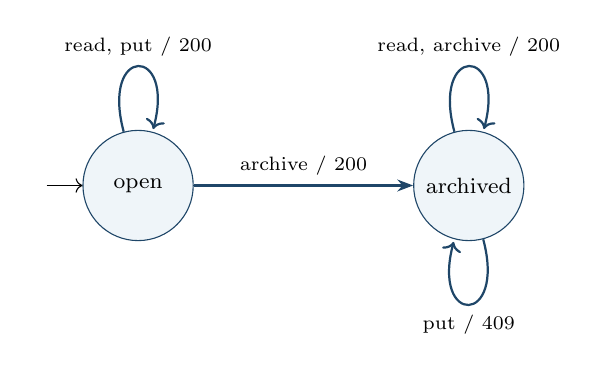
\begin{tikzpicture}[every state/.style={draw=inkblue,fill=pale,font=\footnotesize,minimum size=14mm}]
\node[state,initial,initial text={}] (o) at (0,0) {open};
\node[state] (a) at (4.2,0) {archived};
\draw[arr] (o) edge[loop above] node[above,font=\scriptsize]{read, put / 200}(o);
\draw[arr] (o)--node[above,font=\scriptsize]{archive / 200}(a);
\draw[arr] (a) edge[loop above] node[above,font=\scriptsize]{read, archive / 200}(a);
\draw[arr] (a) edge[loop below] node[below,font=\scriptsize]{put / 409}(a);
\end{tikzpicture}
\caption{Checked document policy for $h=1$ (event / status). Every usable table induces exactly this machine.}\label{fig:policy}
\end{figure}

This construction is deliberately extreme, and we do not present it as a model of practice. The validator already contains the unique correct answer $f_h$, so an agent adds nothing that the controller could not compute itself. Its purpose is to show that Corollary~\ref{cor:domain} can be discharged \emph{completely}: when the validator is the specification, the coordination guarantees become a correctness guarantee for every published artifact. The LLM workflows below take the opposite position. Their validators do not contain a solution, many different artifacts are accepted, and the gap between acceptance and correctness is measured rather than proved away.

\subsection{Controllers, Formal Model and Proofs}\label{sec:artifact}
\emph{Reference controller.} A Python implementation (\texttt{src/vgc/controller.py}, about 350 lines with its kernel) realizes the transitions of Table~\ref{tab:rules} for the scripted case study. It serializes public actions with one lock. Every action copies a private candidate, installs effects there, recomputes the complete downstream structure (for all configured consumers), and installs the candidate only on success. Observations are canonical JSON that contains the owner, contract, source clause, usable predecessor values and the full membership of the selected findings; context version numbers are excluded because agents do not see them. A separately implemented \emph{trace checker} replays recorded events and re-evaluates state continuity, ranked availability, exact observations, dispatch identities and counters, provenance, authority, rollback and publication snapshots.

\emph{Generic kernel.} A second implementation (\texttt{src/vgc/graph.py}, \GraphLines{} lines) applies the same discipline to an arbitrary ranked DAG of jobs. A job is declared by its rank, prerequisites, owner, contract, read-set function, context selector and validator. Validation runs outside the lock on the immutable dispatched observation, and the currentness and authority guard is rechecked atomically before the write (OCC). The kernel also implements the coarser strategies of RQ2 and an ungated scheduler for Proposition~\ref{prop:eager}. We tested it \emph{differentially} against the reference controller. On all \DiffRuns{} RQ2 change streams (\DiffChanges{} changes, five strategies), both implementations dispatched exactly the same number of requests after every change and accepted identical values.

\emph{Formal model.} \texttt{Core.tla} and \texttt{AsyncController.tla} formalize ranked prerequisites, exact observations, historical acceptance, episode counters, request history, suspension, contract and authority changes, and publication evidence. The value relation is abstract: a proposal is valid when it equals the observed source value. This abstraction is sufficient because the protocol properties quantify over the validator, so any total validator yields the same transition structure. \texttt{AtomicController.tla} specifies $\mathcal A$, and \texttt{Refinement.tla} defines the mapping $\alpha$ of~\eqref{eq:alpha} and the property that \texttt{AsyncController} implements $\mathcal A$ under $\alpha$.

\emph{Mechanized lemmas and their limits.} Four TLAPS modules check individual proof steps. \texttt{Budget} bounds the counter within one episode. \texttt{ControllerSafety} shows that the commit guard implies a current, authorized, valid commit. \texttt{StructuralKernelProofs} establishes coverage, unique producers and reference range under the hypotheses of Theorem~\ref{thm:kernel}. \texttt{DocumentPolicyProofs} establishes validator equivalence, archive absorption and the archived-\textsf{put} conflict. These are single-step lemmas, not the inductive invariant. Three technical obstacles stand in the way of a parameterized TLAPS proof of Theorem~\ref{thm:safety}. First, usability~\eqref{eq:usable} is defined by a \texttt{RECURSIVE} operator over the prerequisite relation, which the TLAPS back ends do not support; it must be rewritten as a recursive function over a well-founded rank and accompanied by an induction principle. Second, the budget invariant counts history elements per (job, episode) with \texttt{Cardinality}, which requires finite-set reasoning that the SMT back ends handle poorly. Third, \texttt{Reconcile} updates seven nested record fields at once, which produces large proof obligations. We therefore check the refinement and the invariants with TLC on instances of up to \TLCExtMaxJobs{} jobs and \TLCExtMaxStates{} distinct states (RQ4), and leave the parameterized proof as the main verification task (Section~\ref{sec:limitations}).

\subsection{Workflows with Real LLM Proposers}\label{sec:llm-workflows}
\emph{LLM document-service workflow (RQ5).} For each service document $d$ the generic kernel creates three jobs. \emph{design/$d$} returns a JSON object with the identifier type, the five operation names and the HTTP status code for each of five situations. Its validator checks the schema and that every status code agrees with the clauses. \emph{implementation/$d$} returns free-form Python source code for a class \texttt{DocumentStore}. \emph{verification/$d$} returns a free-form test suite \texttt{test\_*(make)}. The authoritative inputs are four natural-language clauses per service, one of which (R03) states whether overwriting an archived document is refused with 409 or allowed. A shared context holds path-traversal findings for some services and, after a feedback epoch, workspace conventions. The global predicate requires one identifier convention across all services, a joint constraint that independently working design agents can violate.

The validators do not contain a solution. Code is checked by property-based testing~\citep{claessen2000quickcheck}: 120 seeded random operation sequences, including invalid and malicious identifiers, are run against the generated class and against a 43-line abstract model of the clauses. The first divergence is shrunk by delta debugging~\citep{zeller2002simplifying} to a minimal failing sequence and returned to the agent as feedback. Tests must pass on the abstract model and on the accepted implementation, and they must fail on at least three of four seeded mutants of the model (policy inverted, \texttt{put} ignored, missing document reported as 200, duplicate creation allowed). All generated code runs in a separate interpreter with memory, CPU and file-descriptor limits; it is never imported into the controller. Many different programs pass. Section~\ref{sec:rq5} reports how many structurally distinct implementations were accepted.

\emph{Benchmark workflow (RQ6).} For each task of HumanEval+ (164 tasks) and MBPP+ (378 tasks)~\citep{evalplus,chen2021humaneval,austin2021mbpp}, the kernel creates \emph{code/$t$} and \emph{tests/$t$}. The declared validator of \emph{code/$t$} is the benchmark's \emph{base} test inputs: outputs of the reference solution, computed in the sandbox before any generated code is loaded, compared as in EvalPlus. The first failing case is returned as feedback. \emph{tests/$t$} must define at least three assertion-based tests that pass on the reference solution and on the accepted code. The benchmark's \emph{plus} inputs (up to \BenchMaxPlus{} per task) are never seen by the controller. They serve only as the ground truth with which we measure how often a validator-accepted value is wrong.


% =====================================================================
\section{Evaluation}\label{sec:evaluation}

\subsection{Research Questions}
The guarantees of Section~\ref{sec:guarantees} are proved on paper. The evaluation asks whether they hold in executable instantiations, whether each mechanism is necessary, what exactness buys, and what happens with real language models. RQ1 and RQ3 are \emph{verification} activities (mutation-based guard-necessity checks and conformance tests), not empirical claims about multi-agent practice; RQ5 and RQ6 provide the latter.
\begin{itemize}
\item[\RQ{1}] \emph{Guard necessity.} Does the controller preserve its safety properties under adversarial executions, and does removing any single mechanism break the property it is meant to protect?
\item[\RQ{2}] \emph{Locality, cost and scheduling.} How much generation does exact dependency tracking avoid, on independent and on coupled workspaces, and how does the upstream gate affect repair cost under asynchronous scheduling?
\item[\RQ{3}] \emph{Conformance.} Does the reference implementation handle each class of workflow change exactly as the semantics prescribes?
\item[\RQ{4}] \emph{Assurance.} What do the mechanized proofs and bounded model checks establish, and what remains open?
\item[\RQ{5}] \emph{Real LLM proposers.} With real models generating designs, code and tests, how often are proposals rejected, repaired, globally inconsistent, or stale, how often does early cutoff apply, and what does exactness save?
\item[\RQ{6}] \emph{Validator strength on standard benchmarks.} On HumanEval+ and MBPP+, how often does a value accepted by the declared validator fail stronger tests, and how often are regenerated values equal?
\end{itemize}

\subsection{Experimental Setup}
\emph{Subjects.} RQ1--RQ4 use the scripted case study (Section~\ref{sec:case-study}), the generic kernel and the TLA$^+$ model. RQ5 and RQ6 use the LLM workflows of Section~\ref{sec:llm-workflows} with the generic kernel.

\emph{Scripted and real proposers.} For RQ1--RQ3 the proposal source is a script, for two reasons. The safety guarantees quantify over \emph{all} proposals, so an adversarial script that can return anything is the stronger test. And deterministic proposals make every run reproducible from its seed. The adversarial provider returns valid proposals, locally valid but structurally or jointly inconsistent proposals, malformed values, and plausible answers to a \emph{different} policy question, and it delivers replies late, out of order, duplicated or never. Scripts cannot answer how often real models produce such proposals, whether early cutoff ever applies to stochastic outputs, or what the savings are worth in tokens and time. RQ5 and RQ6 therefore use real models. They run locally through Ollama~\citep{ollama} with fixed model digests, per-request seeds and logged responses: \texttt{qwen2.5-coder:7b}~\citep{hui2024qwen25coder}, \texttt{llama3.1:8b}~\citep{grattafiori2024llama3}, \texttt{gemma2:9b}~\citep{gemma2024gemma2}, \texttt{phi4:14b}~\citep{abdin2024phi4} and \texttt{mistral-small:24b} on NVIDIA H100 and A100 GPUs of the Digital Research Alliance of Canada, and additionally \texttt{qwen3-coder:30b}~\citep{yang2025qwen3} and \texttt{gpt-oss:20b}~\citep{openai2025gptoss} on a local NVIDIA GB10 for RQ5.

\emph{RQ1 ablation harness.} We drive the reference controller and ten variants that each remove exactly one mechanism (two remove both obsolete-reply defenses, as in the formal mutants). An eleventh variant implements the enabled-only semantics, with structural checks for enabled consumers only (Section~\ref{sec:deferred}). Every variant reuses the reference code and overrides only the affected check. Each run starts with one to three documents, budget $k=2$, and executes \AblSteps{} random actions: dispatch; delivery in random order, possibly duplicated; timeout; source edits that flip a policy, add or delete a document; context updates, including equal-content rewrites, unselected findings and availability toggles; contract changes; owner revocation and regrant; adding or removing the reviewer; cooperative repair bursts; and publication attempts. All variants use the same \AblRuns{} seeds. An \emph{independent oracle} judges the state after every transaction. It recomputes each job's observation from the authoritative inputs, remembers the observation each request was dispatched against, tracks episodes itself, and never reads the controller's keys. It checks seven safety properties and one liveness property:
P1 no value is usable whose evidence was produced for a different or unavailable observation (and no request is sent on one);
P2 no usable value is invalid for its current observation;
P3 no value is usable while a prerequisite is unusable;
P4 no value from a revoked owner is usable;
P5 no ill-typed structure is installed for an active consumer;
P6 no episode receives more than $k$ requests;
P7 every published snapshot is fully usable and satisfies $G$;
L1 no authorized edit or context change is refused because of a committed generated value.
The violation rates are a property of the action generator's sampling distribution, not of any deployment. What matters is whether a property is violated at all.

\emph{RQ2 harnesses.} Five strategies share validators, scheduler and guards and differ \emph{only} in what a job's key observes: (i) \emph{Exact} (this paper); (ii) \emph{No early cutoff}, where a job also depends on the identity of each upstream acceptance, as in timestamp-based build tools; (iii) \emph{Version-keyed context}, where context readers depend on the global context version; (iv) \emph{Whole workspace}, where every job sees all inputs and the whole context, as in shared-message-pool frameworks; and (v) \emph{Full regeneration}. The \emph{independent} workspace replicates the four-view chain for $N\in\{1,2,4,\ldots,\CostMaxN\}$ mutually independent documents, with \CostSeeds{} seeded streams of \CostChanges{} changes per size. The \emph{coupled} workspace has \CoupledModules{} modules whose design jobs read $f\in\{0,1,2,4,8\}$ of \CoupledShared{} shared data-model components. Each component is a two-job chain, a specification with fields and a description followed by a derived schema of the fields. Its change stream adds semantic edits (a new field) and cosmetic edits (description only) of shared components. The \emph{scheduling} harness uses layered lattices of depth $d\le\SchedMaxDepth$ and width $w\le\SchedMaxWidth$ in which every node reads all nodes of the previous layer. After one root edit it repairs under random request latencies with unlimited parallelism, with and without the upstream gate (\SchedSeeds{} seeds per cell). Providers are deterministic functions of the observation, so all strategies must accept identical values; we check this after every change.

\emph{RQ3, RQ4.} The \Scenarios{} scenarios and their expectations are fixed in advance in \texttt{campaign.json}. Model checking uses TLC (version \TLCExtVersion). Proofs use TLAPS with its bundled Z3 4.8.9 in strict mode with fingerprints erased. Python \PythonVersion{} was used for the controllers.

\emph{RQ5 protocol.} For each model, we run \emph{completion} trials: a fresh four-service workspace with random policies and findings is repaired from scratch with $k=3$ and validator feedback. If the barrier reports a conflict, one feedback epoch promotes the majority identifier type to a workspace convention. In \emph{stale} trials, an implementation request is dispatched, R03 is flipped half a second later while the model is still generating, and the late reply is delivered. In \emph{cutoff} trials, at temperatures 0 and 0.7, the design contract and then the implementation contract are replaced by a reworded instruction with the same meaning, and we compare the regenerated value with the previous one. In \emph{cost} runs, one fixed stream of eight changes is applied under four strategies. All other generation settings are fixed (temperature 0.7, at most 2,500 output tokens).

\emph{RQ6 protocol.} Each model runs all \BenchTasks{} tasks once at temperature 0.2 with $k=3$. After the initial repair, every code job's contract is replaced by a reworded instruction with the same meaning, and the workflow is repaired again.

% ---------------------------------------------------------------------
\subsection{RQ1: Necessity of Each Guard}\label{sec:rq1}
\emph{Bounded model checking.} Nine one-job baselines, nine one-job mutants and five nonvacuity witnesses (Table~\ref{tab:tlc} in Appendix~\ref{app:tables}) all met their expectation with the current TLC release: \TLCMutantsCaught{} mutants violated their targeted property, and the two that remove a single obsolete-reply defense survive because the other defense still blocks the stale commit. Table~\ref{tab:tlc-ext} adds multi-job instances (RQ4). There, each of the \TLCExtMutants{} mutant configurations, every mutant on chains of two and three jobs and on a four-job diamond, behaves as predicted: \TLCExtMutantsCaught{} violate their targeted property within a few actions, and only the six configurations that remove a single obsolete-reply defense survive, because the other defense still blocks the stale commit.


\emph{Implementation-level ablation.} Fig.~\ref{fig:ablation} asks the same question of the implementation, with several documents, concurrent replies and adversarial proposals. Across \AblRuns{} runs, the reference controller showed \textbf{no} violation of any property (\FullViolRuns{} runs) and refused no authorized change (\FullRefusals{} refusals). It still published in \FullPubRuns{} runs (\FullPublications{} publications), so the absence of violations is not due to inactivity. Every non-redundant ablation was detected on the property it targets:
\begin{itemize}
\item removing both obsolete-reply defenses exposed stale values in \ObsoleteStalePct\% of runs, and in \ObsoleteInvalidPct\% values that were \emph{invalid} for the current input;
\item omitting the contract from the key did so in \ContractStalePct\%, and omitting selected context in \ContextStalePct\%;
\item removing the upstream gate exposed values over stale prerequisites in \UpstreamPct\%;
\item ignoring authority exposed revoked owners' values in \AuthorityPct\%;
\item skipping candidate normalization installed ill-typed structure in \CandidatePct\%;
\item resetting budgets exceeded $k$ requests per episode in \BudgetPct\%;
\item dropping the global predicate published inconsistent snapshots in \GlobalPublishPct\%;
\item checking structural expressions only for enabled consumers refused \EnabledOnlyRefusals{} authorized changes in \EnabledOnlyRuns{} runs (L1), without any safety violation.
\end{itemize}
Removing \emph{one} obsolete-reply defense again produced no violation, which replicates the model-checking result at implementation scale. Several ablations also violate secondary properties; stale contracts, for example, propagate into P3 and P7, because a stale value feeds its descendants and can reach publication.

\begin{figure}[pos=!htbp]
\centering
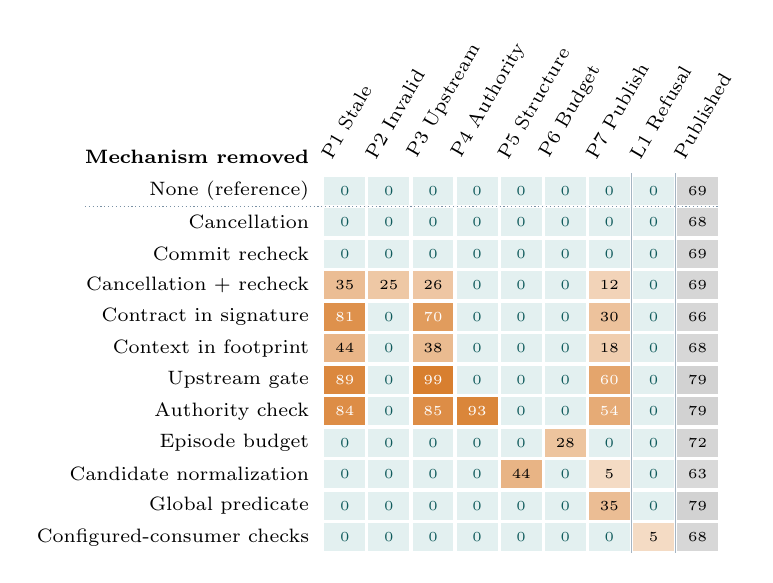
\begin{tikzpicture}
\node[rotate=60,anchor=south west,font=\scriptsize] at (-0.12,0.02) {P1 Stale};
\node[rotate=60,anchor=south west,font=\scriptsize] at (0.44,0.02) {P2 Invalid};
\node[rotate=60,anchor=south west,font=\scriptsize] at (1.00,0.02) {P3 Upstream};
\node[rotate=60,anchor=south west,font=\scriptsize] at (1.56,0.02) {P4 Authority};
\node[rotate=60,anchor=south west,font=\scriptsize] at (2.12,0.02) {P5 Structure};
\node[rotate=60,anchor=south west,font=\scriptsize] at (2.68,0.02) {P6 Budget};
\node[rotate=60,anchor=south west,font=\scriptsize] at (3.24,0.02) {P7 Publish};
\node[rotate=60,anchor=south west,font=\scriptsize] at (3.80,0.02) {L1 Refusal};
\node[rotate=60,anchor=south west,font=\scriptsize] at (4.36,0.02) {Published};
\node[anchor=east,font=\scriptsize] at (-0.33,-0.20) {None (reference)};
\fill[resultteal!12!white] (-0.26,-0.38) rectangle ++(0.52,0.36);
\node[font=\tiny,text=resultteal!70!black] at (0.00,-0.20) {0};
\fill[resultteal!12!white] (0.30,-0.38) rectangle ++(0.52,0.36);
\node[font=\tiny,text=resultteal!70!black] at (0.56,-0.20) {0};
\fill[resultteal!12!white] (0.86,-0.38) rectangle ++(0.52,0.36);
\node[font=\tiny,text=resultteal!70!black] at (1.12,-0.20) {0};
\fill[resultteal!12!white] (1.42,-0.38) rectangle ++(0.52,0.36);
\node[font=\tiny,text=resultteal!70!black] at (1.68,-0.20) {0};
\fill[resultteal!12!white] (1.98,-0.38) rectangle ++(0.52,0.36);
\node[font=\tiny,text=resultteal!70!black] at (2.24,-0.20) {0};
\fill[resultteal!12!white] (2.54,-0.38) rectangle ++(0.52,0.36);
\node[font=\tiny,text=resultteal!70!black] at (2.80,-0.20) {0};
\fill[resultteal!12!white] (3.10,-0.38) rectangle ++(0.52,0.36);
\node[font=\tiny,text=resultteal!70!black] at (3.36,-0.20) {0};
\fill[resultteal!12!white] (3.66,-0.38) rectangle ++(0.52,0.36);
\node[font=\tiny,text=resultteal!70!black] at (3.92,-0.20) {0};
\fill[gray!32!white] (4.22,-0.38) rectangle ++(0.52,0.36);
\node[font=\tiny,text=black] at (4.48,-0.20) {69};
\draw[inkblue!60,densely dotted] (-3.3,-0.40) -- (4.76,-0.40);
\node[anchor=east,font=\scriptsize] at (-0.33,-0.60) {Cancellation};
\fill[resultteal!12!white] (-0.26,-0.78) rectangle ++(0.52,0.36);
\node[font=\tiny,text=resultteal!70!black] at (0.00,-0.60) {0};
\fill[resultteal!12!white] (0.30,-0.78) rectangle ++(0.52,0.36);
\node[font=\tiny,text=resultteal!70!black] at (0.56,-0.60) {0};
\fill[resultteal!12!white] (0.86,-0.78) rectangle ++(0.52,0.36);
\node[font=\tiny,text=resultteal!70!black] at (1.12,-0.60) {0};
\fill[resultteal!12!white] (1.42,-0.78) rectangle ++(0.52,0.36);
\node[font=\tiny,text=resultteal!70!black] at (1.68,-0.60) {0};
\fill[resultteal!12!white] (1.98,-0.78) rectangle ++(0.52,0.36);
\node[font=\tiny,text=resultteal!70!black] at (2.24,-0.60) {0};
\fill[resultteal!12!white] (2.54,-0.78) rectangle ++(0.52,0.36);
\node[font=\tiny,text=resultteal!70!black] at (2.80,-0.60) {0};
\fill[resultteal!12!white] (3.10,-0.78) rectangle ++(0.52,0.36);
\node[font=\tiny,text=resultteal!70!black] at (3.36,-0.60) {0};
\fill[resultteal!12!white] (3.66,-0.78) rectangle ++(0.52,0.36);
\node[font=\tiny,text=resultteal!70!black] at (3.92,-0.60) {0};
\fill[gray!31!white] (4.22,-0.78) rectangle ++(0.52,0.36);
\node[font=\tiny,text=black] at (4.48,-0.60) {68};
\node[anchor=east,font=\scriptsize] at (-0.33,-1.00) {Commit recheck};
\fill[resultteal!12!white] (-0.26,-1.18) rectangle ++(0.52,0.36);
\node[font=\tiny,text=resultteal!70!black] at (0.00,-1.00) {0};
\fill[resultteal!12!white] (0.30,-1.18) rectangle ++(0.52,0.36);
\node[font=\tiny,text=resultteal!70!black] at (0.56,-1.00) {0};
\fill[resultteal!12!white] (0.86,-1.18) rectangle ++(0.52,0.36);
\node[font=\tiny,text=resultteal!70!black] at (1.12,-1.00) {0};
\fill[resultteal!12!white] (1.42,-1.18) rectangle ++(0.52,0.36);
\node[font=\tiny,text=resultteal!70!black] at (1.68,-1.00) {0};
\fill[resultteal!12!white] (1.98,-1.18) rectangle ++(0.52,0.36);
\node[font=\tiny,text=resultteal!70!black] at (2.24,-1.00) {0};
\fill[resultteal!12!white] (2.54,-1.18) rectangle ++(0.52,0.36);
\node[font=\tiny,text=resultteal!70!black] at (2.80,-1.00) {0};
\fill[resultteal!12!white] (3.10,-1.18) rectangle ++(0.52,0.36);
\node[font=\tiny,text=resultteal!70!black] at (3.36,-1.00) {0};
\fill[resultteal!12!white] (3.66,-1.18) rectangle ++(0.52,0.36);
\node[font=\tiny,text=resultteal!70!black] at (3.92,-1.00) {0};
\fill[gray!32!white] (4.22,-1.18) rectangle ++(0.52,0.36);
\node[font=\tiny,text=black] at (4.48,-1.00) {69};
\node[anchor=east,font=\scriptsize] at (-0.33,-1.40) {Cancellation + recheck};
\fill[resultamber!51!white] (-0.26,-1.58) rectangle ++(0.52,0.36);
\node[font=\tiny,text=black] at (0.00,-1.40) {35};
\fill[resultamber!43!white] (0.30,-1.58) rectangle ++(0.52,0.36);
\node[font=\tiny,text=black] at (0.56,-1.40) {25};
\fill[resultamber!44!white] (0.86,-1.58) rectangle ++(0.52,0.36);
\node[font=\tiny,text=black] at (1.12,-1.40) {26};
\fill[resultteal!12!white] (1.42,-1.58) rectangle ++(0.52,0.36);
\node[font=\tiny,text=resultteal!70!black] at (1.68,-1.40) {0};
\fill[resultteal!12!white] (1.98,-1.58) rectangle ++(0.52,0.36);
\node[font=\tiny,text=resultteal!70!black] at (2.24,-1.40) {0};
\fill[resultteal!12!white] (2.54,-1.58) rectangle ++(0.52,0.36);
\node[font=\tiny,text=resultteal!70!black] at (2.80,-1.40) {0};
\fill[resultamber!34!white] (3.10,-1.58) rectangle ++(0.52,0.36);
\node[font=\tiny,text=black] at (3.36,-1.40) {12};
\fill[resultteal!12!white] (3.66,-1.58) rectangle ++(0.52,0.36);
\node[font=\tiny,text=resultteal!70!black] at (3.92,-1.40) {0};
\fill[gray!32!white] (4.22,-1.58) rectangle ++(0.52,0.36);
\node[font=\tiny,text=black] at (4.48,-1.40) {69};
\node[anchor=east,font=\scriptsize] at (-0.33,-1.80) {Contract in signature};
\fill[resultamber!85!white] (-0.26,-1.98) rectangle ++(0.52,0.36);
\node[font=\tiny,text=white] at (0.00,-1.80) {81};
\fill[resultteal!12!white] (0.30,-1.98) rectangle ++(0.52,0.36);
\node[font=\tiny,text=resultteal!70!black] at (0.56,-1.80) {0};
\fill[resultamber!77!white] (0.86,-1.98) rectangle ++(0.52,0.36);
\node[font=\tiny,text=white] at (1.12,-1.80) {70};
\fill[resultteal!12!white] (1.42,-1.98) rectangle ++(0.52,0.36);
\node[font=\tiny,text=resultteal!70!black] at (1.68,-1.80) {0};
\fill[resultteal!12!white] (1.98,-1.98) rectangle ++(0.52,0.36);
\node[font=\tiny,text=resultteal!70!black] at (2.24,-1.80) {0};
\fill[resultteal!12!white] (2.54,-1.98) rectangle ++(0.52,0.36);
\node[font=\tiny,text=resultteal!70!black] at (2.80,-1.80) {0};
\fill[resultamber!47!white] (3.10,-1.98) rectangle ++(0.52,0.36);
\node[font=\tiny,text=black] at (3.36,-1.80) {30};
\fill[resultteal!12!white] (3.66,-1.98) rectangle ++(0.52,0.36);
\node[font=\tiny,text=resultteal!70!black] at (3.92,-1.80) {0};
\fill[gray!31!white] (4.22,-1.98) rectangle ++(0.52,0.36);
\node[font=\tiny,text=black] at (4.48,-1.80) {66};
\node[anchor=east,font=\scriptsize] at (-0.33,-2.20) {Context in footprint};
\fill[resultamber!57!white] (-0.26,-2.38) rectangle ++(0.52,0.36);
\node[font=\tiny,text=black] at (0.00,-2.20) {44};
\fill[resultteal!12!white] (0.30,-2.38) rectangle ++(0.52,0.36);
\node[font=\tiny,text=resultteal!70!black] at (0.56,-2.20) {0};
\fill[resultamber!53!white] (0.86,-2.38) rectangle ++(0.52,0.36);
\node[font=\tiny,text=black] at (1.12,-2.20) {38};
\fill[resultteal!12!white] (1.42,-2.38) rectangle ++(0.52,0.36);
\node[font=\tiny,text=resultteal!70!black] at (1.68,-2.20) {0};
\fill[resultteal!12!white] (1.98,-2.38) rectangle ++(0.52,0.36);
\node[font=\tiny,text=resultteal!70!black] at (2.24,-2.20) {0};
\fill[resultteal!12!white] (2.54,-2.38) rectangle ++(0.52,0.36);
\node[font=\tiny,text=resultteal!70!black] at (2.80,-2.20) {0};
\fill[resultamber!38!white] (3.10,-2.38) rectangle ++(0.52,0.36);
\node[font=\tiny,text=black] at (3.36,-2.20) {18};
\fill[resultteal!12!white] (3.66,-2.38) rectangle ++(0.52,0.36);
\node[font=\tiny,text=resultteal!70!black] at (3.92,-2.20) {0};
\fill[gray!31!white] (4.22,-2.38) rectangle ++(0.52,0.36);
\node[font=\tiny,text=black] at (4.48,-2.20) {68};
\node[anchor=east,font=\scriptsize] at (-0.33,-2.60) {Upstream gate};
\fill[resultamber!92!white] (-0.26,-2.78) rectangle ++(0.52,0.36);
\node[font=\tiny,text=white] at (0.00,-2.60) {89};
\fill[resultteal!12!white] (0.30,-2.78) rectangle ++(0.52,0.36);
\node[font=\tiny,text=resultteal!70!black] at (0.56,-2.60) {0};
\fill[resultamber!99!white] (0.86,-2.78) rectangle ++(0.52,0.36);
\node[font=\tiny,text=white] at (1.12,-2.60) {99};
\fill[resultteal!12!white] (1.42,-2.78) rectangle ++(0.52,0.36);
\node[font=\tiny,text=resultteal!70!black] at (1.68,-2.60) {0};
\fill[resultteal!12!white] (1.98,-2.78) rectangle ++(0.52,0.36);
\node[font=\tiny,text=resultteal!70!black] at (2.24,-2.60) {0};
\fill[resultteal!12!white] (2.54,-2.78) rectangle ++(0.52,0.36);
\node[font=\tiny,text=resultteal!70!black] at (2.80,-2.60) {0};
\fill[resultamber!70!white] (3.10,-2.78) rectangle ++(0.52,0.36);
\node[font=\tiny,text=white] at (3.36,-2.60) {60};
\fill[resultteal!12!white] (3.66,-2.78) rectangle ++(0.52,0.36);
\node[font=\tiny,text=resultteal!70!black] at (3.92,-2.60) {0};
\fill[gray!35!white] (4.22,-2.78) rectangle ++(0.52,0.36);
\node[font=\tiny,text=black] at (4.48,-2.60) {79};
\node[anchor=east,font=\scriptsize] at (-0.33,-3.00) {Authority check};
\fill[resultamber!88!white] (-0.26,-3.18) rectangle ++(0.52,0.36);
\node[font=\tiny,text=white] at (0.00,-3.00) {84};
\fill[resultteal!12!white] (0.30,-3.18) rectangle ++(0.52,0.36);
\node[font=\tiny,text=resultteal!70!black] at (0.56,-3.00) {0};
\fill[resultamber!88!white] (0.86,-3.18) rectangle ++(0.52,0.36);
\node[font=\tiny,text=white] at (1.12,-3.00) {85};
\fill[resultamber!94!white] (1.42,-3.18) rectangle ++(0.52,0.36);
\node[font=\tiny,text=white] at (1.68,-3.00) {93};
\fill[resultteal!12!white] (1.98,-3.18) rectangle ++(0.52,0.36);
\node[font=\tiny,text=resultteal!70!black] at (2.24,-3.00) {0};
\fill[resultteal!12!white] (2.54,-3.18) rectangle ++(0.52,0.36);
\node[font=\tiny,text=resultteal!70!black] at (2.80,-3.00) {0};
\fill[resultamber!65!white] (3.10,-3.18) rectangle ++(0.52,0.36);
\node[font=\tiny,text=white] at (3.36,-3.00) {54};
\fill[resultteal!12!white] (3.66,-3.18) rectangle ++(0.52,0.36);
\node[font=\tiny,text=resultteal!70!black] at (3.92,-3.00) {0};
\fill[gray!35!white] (4.22,-3.18) rectangle ++(0.52,0.36);
\node[font=\tiny,text=black] at (4.48,-3.00) {79};
\node[anchor=east,font=\scriptsize] at (-0.33,-3.40) {Episode budget};
\fill[resultteal!12!white] (-0.26,-3.58) rectangle ++(0.52,0.36);
\node[font=\tiny,text=resultteal!70!black] at (0.00,-3.40) {0};
\fill[resultteal!12!white] (0.30,-3.58) rectangle ++(0.52,0.36);
\node[font=\tiny,text=resultteal!70!black] at (0.56,-3.40) {0};
\fill[resultteal!12!white] (0.86,-3.58) rectangle ++(0.52,0.36);
\node[font=\tiny,text=resultteal!70!black] at (1.12,-3.40) {0};
\fill[resultteal!12!white] (1.42,-3.58) rectangle ++(0.52,0.36);
\node[font=\tiny,text=resultteal!70!black] at (1.68,-3.40) {0};
\fill[resultteal!12!white] (1.98,-3.58) rectangle ++(0.52,0.36);
\node[font=\tiny,text=resultteal!70!black] at (2.24,-3.40) {0};
\fill[resultamber!46!white] (2.54,-3.58) rectangle ++(0.52,0.36);
\node[font=\tiny,text=black] at (2.80,-3.40) {28};
\fill[resultteal!12!white] (3.10,-3.58) rectangle ++(0.52,0.36);
\node[font=\tiny,text=resultteal!70!black] at (3.36,-3.40) {0};
\fill[resultteal!12!white] (3.66,-3.58) rectangle ++(0.52,0.36);
\node[font=\tiny,text=resultteal!70!black] at (3.92,-3.40) {0};
\fill[gray!33!white] (4.22,-3.58) rectangle ++(0.52,0.36);
\node[font=\tiny,text=black] at (4.48,-3.40) {72};
\node[anchor=east,font=\scriptsize] at (-0.33,-3.80) {Candidate normalization};
\fill[resultteal!12!white] (-0.26,-3.98) rectangle ++(0.52,0.36);
\node[font=\tiny,text=resultteal!70!black] at (0.00,-3.80) {0};
\fill[resultteal!12!white] (0.30,-3.98) rectangle ++(0.52,0.36);
\node[font=\tiny,text=resultteal!70!black] at (0.56,-3.80) {0};
\fill[resultteal!12!white] (0.86,-3.98) rectangle ++(0.52,0.36);
\node[font=\tiny,text=resultteal!70!black] at (1.12,-3.80) {0};
\fill[resultteal!12!white] (1.42,-3.98) rectangle ++(0.52,0.36);
\node[font=\tiny,text=resultteal!70!black] at (1.68,-3.80) {0};
\fill[resultamber!58!white] (1.98,-3.98) rectangle ++(0.52,0.36);
\node[font=\tiny,text=black] at (2.24,-3.80) {44};
\fill[resultteal!12!white] (2.54,-3.98) rectangle ++(0.52,0.36);
\node[font=\tiny,text=resultteal!70!black] at (2.80,-3.80) {0};
\fill[resultamber!28!white] (3.10,-3.98) rectangle ++(0.52,0.36);
\node[font=\tiny,text=black] at (3.36,-3.80) {5};
\fill[resultteal!12!white] (3.66,-3.98) rectangle ++(0.52,0.36);
\node[font=\tiny,text=resultteal!70!black] at (3.92,-3.80) {0};
\fill[gray!30!white] (4.22,-3.98) rectangle ++(0.52,0.36);
\node[font=\tiny,text=black] at (4.48,-3.80) {63};
\node[anchor=east,font=\scriptsize] at (-0.33,-4.20) {Global predicate};
\fill[resultteal!12!white] (-0.26,-4.38) rectangle ++(0.52,0.36);
\node[font=\tiny,text=resultteal!70!black] at (0.00,-4.20) {0};
\fill[resultteal!12!white] (0.30,-4.38) rectangle ++(0.52,0.36);
\node[font=\tiny,text=resultteal!70!black] at (0.56,-4.20) {0};
\fill[resultteal!12!white] (0.86,-4.38) rectangle ++(0.52,0.36);
\node[font=\tiny,text=resultteal!70!black] at (1.12,-4.20) {0};
\fill[resultteal!12!white] (1.42,-4.38) rectangle ++(0.52,0.36);
\node[font=\tiny,text=resultteal!70!black] at (1.68,-4.20) {0};
\fill[resultteal!12!white] (1.98,-4.38) rectangle ++(0.52,0.36);
\node[font=\tiny,text=resultteal!70!black] at (2.24,-4.20) {0};
\fill[resultteal!12!white] (2.54,-4.38) rectangle ++(0.52,0.36);
\node[font=\tiny,text=resultteal!70!black] at (2.80,-4.20) {0};
\fill[resultamber!51!white] (3.10,-4.38) rectangle ++(0.52,0.36);
\node[font=\tiny,text=black] at (3.36,-4.20) {35};
\fill[resultteal!12!white] (3.66,-4.38) rectangle ++(0.52,0.36);
\node[font=\tiny,text=resultteal!70!black] at (3.92,-4.20) {0};
\fill[gray!35!white] (4.22,-4.38) rectangle ++(0.52,0.36);
\node[font=\tiny,text=black] at (4.48,-4.20) {79};
\node[anchor=east,font=\scriptsize] at (-0.33,-4.60) {Configured-consumer checks};
\fill[resultteal!12!white] (-0.26,-4.78) rectangle ++(0.52,0.36);
\node[font=\tiny,text=resultteal!70!black] at (0.00,-4.60) {0};
\fill[resultteal!12!white] (0.30,-4.78) rectangle ++(0.52,0.36);
\node[font=\tiny,text=resultteal!70!black] at (0.56,-4.60) {0};
\fill[resultteal!12!white] (0.86,-4.78) rectangle ++(0.52,0.36);
\node[font=\tiny,text=resultteal!70!black] at (1.12,-4.60) {0};
\fill[resultteal!12!white] (1.42,-4.78) rectangle ++(0.52,0.36);
\node[font=\tiny,text=resultteal!70!black] at (1.68,-4.60) {0};
\fill[resultteal!12!white] (1.98,-4.78) rectangle ++(0.52,0.36);
\node[font=\tiny,text=resultteal!70!black] at (2.24,-4.60) {0};
\fill[resultteal!12!white] (2.54,-4.78) rectangle ++(0.52,0.36);
\node[font=\tiny,text=resultteal!70!black] at (2.80,-4.60) {0};
\fill[resultteal!12!white] (3.10,-4.78) rectangle ++(0.52,0.36);
\node[font=\tiny,text=resultteal!70!black] at (3.36,-4.60) {0};
\fill[resultamber!28!white] (3.66,-4.78) rectangle ++(0.52,0.36);
\node[font=\tiny,text=black] at (3.92,-4.60) {5};
\fill[gray!31!white] (4.22,-4.78) rectangle ++(0.52,0.36);
\node[font=\tiny,text=black] at (4.48,-4.60) {68};
\draw[inkblue!40] (3.64,0.02) -- (3.64,-4.80);
\draw[inkblue!40] (4.20,0.02) -- (4.20,-4.80);
\node[anchor=south east,font=\scriptsize\bfseries] at (-0.33,0.02) {Mechanism removed};
\end{tikzpicture}
\caption{RQ1: implementation-level guard ablation under 300 seeded adversarial executions per variant (120 steps each). Cells give the percentage of runs in which the independent oracle observed at least one violation of property P1--P7 (Section~\ref{sec:rq1}); L1 is the liveness hazard of Section~\ref{sec:deferred} (an authorized change refused because of a committed generated value); the last column gives the percentage of runs that published at least once. The reference controller (top row) shows no violation and no refusal. Removing either obsolete-response defense alone is masked by the other. The bottom row is not a removal but the enabled-only semantics, which checks structural expressions only for enabled consumers.}\label{fig:ablation}
\end{figure}



\emph{A defect found by the campaign.} On an earlier version of our controller, the randomized campaign exposed a defect: \texttt{update\_context} let a normalization exception escape when re-enabled context made a previously committed integer architecture inadmissible (\PreFixApiRuns{} of \PreFixRuns{} runs). Repairing the API alone was not enough. We traced the defect to its semantic root, the deferred-check hazard of Section~\ref{sec:deferred}, and repaired the semantics. The commit guard now checks configured consumers, which removes the refusals entirely, and Theorem~\ref{thm:termination} relies on this rule. The L1 column of Fig.~\ref{fig:ablation} quantifies the hazard under the enabled-only semantics. The episode illustrates why trustworthiness must be engineered across the life-cycle: adversarial testing of the implementation exposed a gap that the paper proof had not covered.

\textbf{Answer to RQ1.} No safety violation occurred in any exhaustive baseline configuration or in the \AblRuns{} adversarial executions of the reference controller. Each ablation of a non-redundant mechanism violated its targeted property, both in the model and in the implementation. The cancellation and recheck defenses are individually redundant but jointly necessary. The configured-consumer structural check removes a liveness hazard of the enabled-only semantics.

% ---------------------------------------------------------------------
\subsection{RQ2: Locality, Cost and Scheduling}\label{sec:rq2}
\emph{Independent workspaces.} Fig.~\ref{fig:cost} and Table~\ref{tab:cost} report requests and observation bytes per change for $N$ mutually independent documents. This topology isolates the effect of the key: with exact keys, a source edit regenerates that document's four jobs, a selected-context change regenerates the two jobs that read the finding, and unselected changes and equal-content rewrites regenerate nothing. Only contract changes touch every job of the changed stage. Because the documents are independent, the ratios to the coarser strategies grow with $N$ \emph{by construction}. At $N=\CostMaxN$, exact keys needed \ExactReqMaxN{} requests per change against \FullReqMaxN{} for full regeneration (\RatioFull$\times$), and the whole-workspace strategy sent \BytesRatioWorkspace$\times$ the observation bytes (\WorkspaceKBMaxN{} vs.\ \ExactKBMaxN{} kB per change). These numbers show what exactness is worth when work is independent. They do not predict savings on coupled software, which the next experiment addresses.

\begin{figure}[pos=!htbp]
\centering
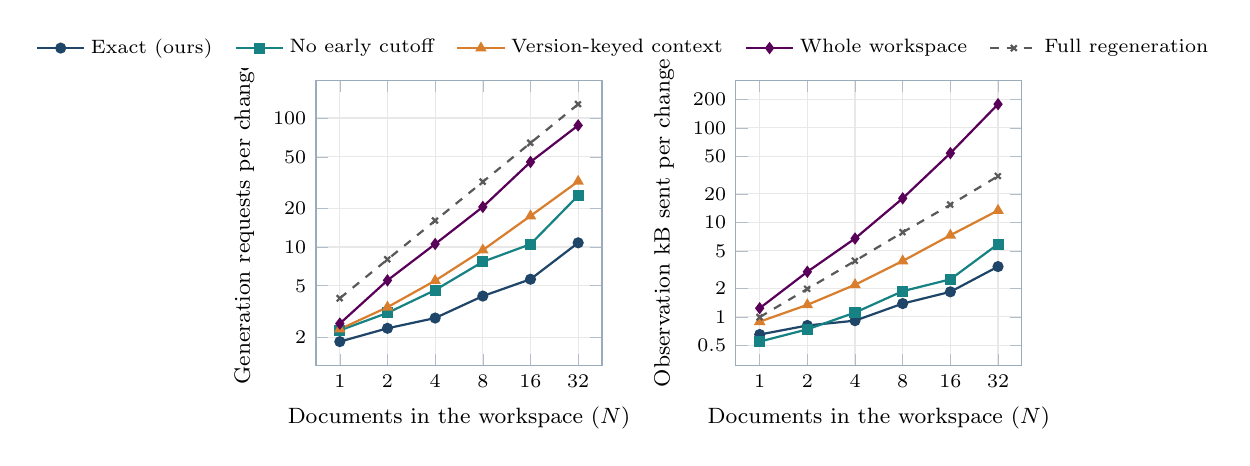
\begin{tikzpicture}
\begin{groupplot}[group style={group size=2 by 1,horizontal sep=1.7cm},vgcplot,width=.43\textwidth,height=5.2cm,
  xmode=log,log basis x=2,ymode=log,xtick={1,2,4,8,16,32},xticklabels={1,2,4,8,16,32},log ticks with fixed point,
  ytick={0.1,0.2,0.5,1,2,5,10,20,50,100,200,500,1000,2000},xlabel={Documents in the workspace ($N$)},
  legend style={at={(1.08,1.04)},anchor=south,legend columns=5,draw=none,/tikz/every even column/.append style={column sep=6pt}}]
\nextgroupplot[ylabel={Generation requests per change}]
\addplot[inkblue,mark=*,thick,mark size=1.6pt] coordinates {(1,1.845) (2,2.34) (4,2.81) (8,4.16) (16,5.62) (32,10.77)};
\addplot[resultteal,mark=square*,thick,mark size=1.6pt] coordinates {(1,2.255) (2,3.08) (4,4.63) (8,7.68) (16,10.5) (32,25.01)};
\addplot[resultamber,mark=triangle*,thick,mark size=1.6pt] coordinates {(1,2.305) (2,3.41) (4,5.48) (8,9.46) (16,17.4) (32,32.24)};
\addplot[violet!70!black,mark=diamond*,thick,mark size=1.6pt] coordinates {(1,2.545) (2,5.51) (4,10.54) (8,20.44) (16,45.6) (32,87.68)};
\addplot[gray!70!black,mark=x,dashed,thick,mark size=1.6pt] coordinates {(1,4) (2,8) (4,16) (8,32) (16,64) (32,128)};
\legend{Exact (ours),No early cutoff,Version-keyed context,Whole workspace,Full regeneration}
\nextgroupplot[ylabel={Observation kB sent per change}]
\addplot[inkblue,mark=*,thick,mark size=1.6pt] coordinates {(1,0.6504) (2,0.8106) (4,0.9113) (8,1.382) (16,1.84) (32,3.404)};
\addplot[resultteal,mark=square*,thick,mark size=1.6pt] coordinates {(1,0.5473) (2,0.7381) (4,1.11) (8,1.87) (16,2.494) (32,5.888)};
\addplot[resultamber,mark=triangle*,thick,mark size=1.6pt] coordinates {(1,0.8893) (2,1.34) (4,2.186) (8,3.899) (16,7.299) (32,13.35)};
\addplot[violet!70!black,mark=diamond*,thick,mark size=1.6pt] coordinates {(1,1.235) (2,2.998) (4,6.741) (8,17.93) (16,53.89) (32,177.7)};
\addplot[gray!70!black,mark=x,dashed,thick,mark size=1.6pt] coordinates {(1,0.9932) (2,1.974) (4,3.907) (8,7.842) (16,15.33) (32,30.82)};
\end{groupplot}
\end{tikzpicture}
\caption{RQ2: generation work per input change as the workspace grows (log--log; mean over 5 seeds $\times$ 40 random changes per size). All strategies share validators, scheduler and guards and differ only in what a job's signature observes; they accepted identical values in every run. Left: dispatched requests. Right: total size of the observations sent to workers, a proxy for prompt input tokens.}\label{fig:cost}
\end{figure}


\begin{table}[pos=!htbp]
\centering
\caption{RQ2: mean generation requests per change by change type for $N=32$ documents. Exact signatures make the cost of source and context changes independent of $N$; contract changes necessarily touch every job of the changed stage. The $N$ documents are mutually independent (no cross-document dependency); Table~\ref{tab:coupled} adds coupling.}\label{tab:cost}
\scriptsize\setlength{\tabcolsep}{2pt}
\begin{tabular*}{\columnwidth}{@{\extracolsep{\fill}}lrrrrr@{}}\toprule
Change type & \rotatebox{70}{Exact (ours)} & \rotatebox{70}{No early cutoff} & \rotatebox{70}{Version-keyed context} & \rotatebox{70}{Whole workspace} & \rotatebox{70}{Full regeneration}\\\midrule
Source clause edit & 4.0 & 4.0 & 4.0 & 128.0 & 128.0\\
Selected finding changed & 2.0 & 2.0 & 64.0 & 128.0 & 128.0\\
Unselected finding changed & 0.0 & 0.0 & 64.0 & 128.0 & 128.0\\
Equal content, new version & 0.0 & 0.0 & 64.0 & 0.0 & 128.0\\
Contract change & 32.0 & 82.9 & 32.0 & 32.0 & 128.0\\
\midrule All changes & 10.8 & 25.0 & 32.2 & 87.7 & 128.0\\
Bytes per request & 316 & 235 & 414 & 2,027 & 241\\
Total kB per change & 3.4 & 5.9 & 13.3 & 177.7 & 30.8\\
\bottomrule\end{tabular*}
\end{table}



\emph{Coupled workspaces.} Table~\ref{tab:coupled} adds coupling through shared data models. Exact keys now pay for exactly the coupled subgraph a change reaches: a semantic edit of a shared model regenerates the model, its schema and, for every dependent module, design, implementation and verification, so its cost grows linearly with the fan-out, from 2 requests at $f=0$ to \CoupledSemanticFmax{} at $f=\CoupledFmax$. A \emph{cosmetic} edit of a shared model, whose schema regenerates to an equal value, costs \CoupledCosmeticExact{} requests with early cutoff and \CoupledCosmeticNoCut{} without. Over the whole stream, exact keys needed \CoupledExactFzero{} requests per change at $f=0$ and \CoupledExactFmax{} at $f=\CoupledFmax$. The coarser strategies needed \CoupledRatioFullFmax$\times$ (full regeneration), \CoupledRatioWorkspaceFmax$\times$ (whole workspace) and \CoupledRatioCutoffFmax$\times$ (no early cutoff) as many requests at the highest coupling. In every run, every request of the exact strategy was caused by a job whose observation had changed. Exact keys do not make coupled changes cheap; they make the cost equal to the size of the affected subgraph.

\begin{table}[pos=!htbp]
\centering
\caption{RQ2 on a coupled workspace: mean generation requests per change for 32 modules sharing 8 data-model components (144 jobs), 5 seeds $\times$ 60 changes per fan-out $f$ (each module's design reads $f$ shared models). Right: an edit of a shared model that adds a field, and one that changes only its description (exact keys / no early cutoff). With exact keys, requests equalled stale episodes in all runs. Per-change-type results are in Table~\ref{tab:coupled-full} (Appendix~\ref{app:tables}).}\label{tab:coupled}
\footnotesize\setlength{\tabcolsep}{3pt}
\begin{tabular*}{\columnwidth}{@{\extracolsep{\fill}}rrrrrrr@{}}\toprule
& \multicolumn{4}{c}{All changes} & \multicolumn{2}{c}{Shared-model edit}\\\cmidrule(lr){2-5}\cmidrule(l){6-7}
$f$ & Exact & No cutoff & Whole ws. & Full & New field & Description\\\midrule
0 & 9.5 & 21.9 & 118.2 & 144.0 & 2.0 & 2.0 / 2.0\\
1 & 10.7 & 21.8 & 120.1 & 144.0 & 14.2 & 2.0 / 12.6\\
2 & 12.5 & 25.8 & 119.4 & 144.0 & 25.6 & 2.0 / 27.6\\
4 & 16.4 & 31.5 & 120.5 & 144.0 & 50.3 & 2.0 / 53.4\\
8 & 22.1 & 42.3 & 121.6 & 144.0 & 98.0 & 2.0 / 98.0\\
\bottomrule\end{tabular*}
\end{table}



\emph{Scheduling.} Table~\ref{tab:sched} tests Theorem~\ref{thm:single} and Proposition~\ref{prop:eager}. With the upstream gate, every affected job started exactly one stale episode and was dispatched once, for every seed and lattice, so requests equal the number of jobs. Without the gate, jobs were dispatched on partially repaired predecessors and re-dispatched as each predecessor committed: up to \SchedEagerReqRatioMax$\times$ the requests and up to \SchedEagerMaxEpisodes{} episodes for a single job, growing with width and depth. The ungated scheduler bought no latency in exchange: makespans differed by at most \SchedMakespanDiffPct\%, because the speculative work was discarded whenever a predecessor changed.

\begin{table}[pos=!htbp]
\centering
\caption{RQ2 scheduling: requests after one root edit on layered lattices (depth $d$, width $w$, every node reads all nodes of the previous layer), mean of 30 seeds with random latencies and unlimited parallelism. Cells: gated requests / ungated requests / worst episodes of one job (ungated). The gated scheduler started exactly one stale episode per affected job in every run (Theorem~\ref{thm:single}); makespans differed by at most 5\%.}\label{tab:sched}
\scriptsize\setlength{\tabcolsep}{3pt}
\begin{tabular*}{\columnwidth}{@{\extracolsep{\fill}}lcccc@{}}\toprule
$d$ & $w=1$ & $w=2$ & $w=3$ & $w=4$\\\midrule
2 & 2 / 2.0 / 1 & 4 / 6.0 / 2 & 6 / 12.0 / 3 & 8 / 20.0 / 4\\
3 & 3 / 3.0 / 1 & 6 / 10.1 / 3 & 9 / 21.3 / 5 & 12 / 36.3 / 5\\
4 & 4 / 4.0 / 1 & 8 / 14.2 / 3 & 12 / 30.8 / 5 & 16 / 52.5 / 6\\
5 & 5 / 5.0 / 1 & 10 / 18.6 / 4 & 15 / 39.9 / 5 & 20 / 69.7 / 7\\
6 & 6 / 6.0 / 1 & 12 / 25.1 / 5 & 18 / 54.3 / 6 & 24 / 85.3 / 7\\
\bottomrule\end{tabular*}
\end{table}



The scenario campaign confirms the mechanism on individual interventions. A repair pass with no relevant change (S02), an unselected context update (S08) and a new context version with equal selected content (S10) caused no request. An architecture contract change repaired to an equal output caused exactly one request, because early cutoff restored the descendants (S16).

\textbf{Answer to RQ2.} Exact keys make the cost of a change equal to the size of the subgraph whose observations it changes. On independent workspaces this is constant in workspace size, and on coupled workspaces it grows with fan-out. Against full regeneration, the saving was \RatioFull$\times$ on \CostMaxN{} independent documents and still \CoupledRatioFullFmax$\times$ at the highest coupling we measured. Early cutoff matters most for changes that do not propagate semantically. The upstream gate makes repair cost independent of scheduling, at no latency cost in our simulations. RQ5 and RQ6 measure what these structural savings mean with stochastic outputs.

% ---------------------------------------------------------------------
\subsection{RQ3: Conformance Under Change}\label{sec:rq3}
Table~\ref{tab:scenarios} groups the \Scenarios{} scenarios by the class of change they exercise. All \ScenarioPasses{} met their predefined expectations. Many expectations are refusals: a discarded late reply (S11--S13), an exhausted episode that earns no new budget (S14), a blocked descendant (S15), a joint conflict (S18), a rolled-back candidate (S19), a reviewer whose addition blocks publication until it has assessed every operation (S20), and a rejected publication based on a stale check (S25). The trace checker admitted all \Scenarios{} recorded traces and rejected all \Corruptions{} deliberately corrupted ones, including acceptance events that hide a source, context or contract change behind a valid value. In S12 the clause changes and then reverts, so the observation returns to its original value. The cancelled request still cannot commit, because the reversion started a new episode: keys alone do not give idempotent delivery, and request identities are needed as well. The expectations were written by the author, so these are conformance tests of the implementation against the semantics, not independent evidence about the semantics itself.

\begin{table}[pos=!htbp]
\centering
\caption{The 28 scripted change scenarios, grouped by the class of change they exercise. Event counts come from the recorded traces: D dispatched requests, A accepted replies, R current rejections or timeouts, X obsolete or duplicate replies discarded, E committed edits/reconfigurations, B refused edits or publications, P publications. A scenario passes when its independently written expectation holds; for several scenarios the expected outcome is a refusal.}\label{tab:scenarios}
\footnotesize\setlength{\tabcolsep}{4pt}
\begin{tabular*}{\textwidth}{@{\extracolsep{\fill}}llcrrrrrrrc@{}}\toprule
Change class & Scenarios (S\#) & Guarantee exercised & D & A & R & X & E & B & P & Pass\\\midrule
Initial completion and no-op repair & 01, 02 & Thm.~\ref{thm:safety}, Lem.~\ref{thm:local} & 8 & 8 & 0 & 0 & 0 & 0 & 1 & 2/2\\
Source edits, additions, deletions & 03, 04, 05, 06, 17 & Thm.~\ref{thm:kernel}, Lem.~\ref{thm:local} & 28 & 28 & 0 & 0 & 6 & 0 & 0 & 5/5\\
Shared-context changes and writers & 07, 08, 09, 10, 24 & Lem.~\ref{thm:local} & 18 & 18 & 0 & 0 & 6 & 1 & 0 & 5/5\\
Obsolete, late, duplicate replies & 11, 12, 13 & Thm.~\ref{thm:safety}(iv), \ref{thm:refinement} & 3 & 0 & 1 & 4 & 3 & 0 & 0 & 3/3\\
Budget exhaustion and blocking & 14, 15 & Thm.~\ref{thm:cost}, \ref{thm:termination} & 4 & 0 & 4 & 0 & 2 & 4 & 0 & 2/2\\
Contract change and early cutoff & 16, 23 & Lem.~\ref{thm:local}, Thm.~\ref{thm:reconfig} & 10 & 9 & 0 & 1 & 3 & 0 & 0 & 2/2\\
Joint conflict, rollback, stale check & 18, 19, 25 & Thm.~\ref{thm:safety}(i),(v) & 14 & 13 & 1 & 0 & 3 & 2 & 0 & 3/3\\
Reviewer and authority changes & 20, 21, 22 & Thm.~\ref{thm:reconfig} & 10 & 9 & 0 & 1 & 4 & 3 & 1 & 3/3\\
Untrusted ingress, observer loss & 26, 27 & Sec.~\ref{sec:extensions} & 4 & 4 & 0 & 0 & 0 & 2 & 1 & 2/2\\
Finite policy language (exhaustive) & 28 & Thm.~\ref{thm:table} & 0 & 0 & 0 & 0 & 0 & 0 & 0 & 1/1\\
\midrule\textbf{All scenarios} & 01--28 & & 99 & 89 & 6 & 6 & 27 & 12 & 3 & 28/28\\
\bottomrule\end{tabular*}
\end{table}



\textbf{Answer to RQ3.} The reference implementation behaved as the semantics prescribes for all ten change classes, including the refusals, and an independent checker confirmed every recorded trace.

% ---------------------------------------------------------------------
\subsection{RQ4: Assurance and Remaining Obligations}\label{sec:rq4}
Table~\ref{tab:assurance} summarizes the mechanized and exhaustive evidence. The four TLAPS modules discharge \ProvedObligations{} obligations with the pinned toolchain (TLAPS 1.6.0-pre, build 5f5037f, Z3 4.8.9; the recorded logs come from this build, and the current upstream release archive no longer matches the pinned checksum, so we did not substitute it). The preserved first development run failed three obligations in two modules: proof steps that lacked explicit references to construction and type assumptions. The repaired modules split those steps and cite the assumptions explicitly, which changed the number of obligations that TLAPS generates (from 21 to 25). Counts are therefore comparable only within one version of a module, and the first-trial sources were not archived; every run now archives its sources. No assumption equivalent to the safety conclusion was added. For the finite policy language, exhaustive enumeration of all \PolicyTables{} typed tables confirmed that the validator accepts exactly one table per policy, and all \EventWords{} event words of length at most six obey the trace properties of Theorem~\ref{thm:table}.

\begin{table}[pos=!htbp]
\centering
\caption{Assurance evidence. For proofs, \emph{Final} counts proved/total obligations in the clean run and \emph{First trial} the preserved failed development run. Executable counts are exhaustive where stated; the other checks cover the recorded executions only.}\label{tab:assurance}
\scriptsize\setlength{\tabcolsep}{2.5pt}
\begin{tabular*}{\columnwidth}{@{\extracolsep{\fill}}>{\raggedright\arraybackslash}p{24mm}>{\raggedright\arraybackslash}p{28mm}rl@{}}\toprule
Artifact & Scope & Final & First trial\\\midrule
\multicolumn{4}{@{}l}{\textit{Mechanized TLAPS lemmas (strict mode, fingerprints erased)}}\\
{\ttfamily Budget} & Counter bound for one episode & 8/8 & 1 of 7 failed\\
{\ttfamily ControllerSafety} & Commit guard implies current, authorized, valid commit & 2/2 & 0 of 2 failed\\
{\ttfamily StructuralKernel} & Kernel coverage, unique producers, reference range & 9/9 & 2 of 6 failed\\
{\ttfamily DocumentPolicy} & Validator equivalence; archived-put conflict & 6/6 & 0 of 6 failed\\
\midrule\multicolumn{4}{@{}l}{\textit{Executable checks}}\\
Policy tables & All typed six-row tables, both policies & 8,192 & exhaustive\\
Event words & All words of length $\le 6$, strict table & 1,093 & exhaustive\\
Trace checker & Recorded scenario traces admitted & 28/28 & --\\
Trace checker & Deliberately corrupted traces rejected & 9/9 & --\\
Regression tests & Transaction-boundary unit tests & 14/14 & --\\
Reproduction & Clean re-runs of packaged archives matched (earlier code version) & 2/2 & --\\
\bottomrule\end{tabular*}
\end{table}



Table~\ref{tab:tlc-ext} reports the multi-job model-checking campaign. It goes beyond the one-job configurations of Table~\ref{tab:tlc}, among which no multi-job instance with environmental changes had more than \TLCMaxStates{} states and all instances with three or more jobs had frozen inputs. The \TLCExtBaselines{} baselines include chains of up to \TLCExtMaxJobs{} jobs, a fan-out, and a diamond whose sink reads two prerequisites. Their inputs change up to twice, with budgets up to two, and they reach \TLCExtMaxStates{} distinct (\TLCExtMaxGenerated{} generated) states. Every baseline satisfies the full safety invariant and the refinement mapping of Theorem~\ref{thm:refinement}. With both obsolete-reply defenses removed, the refinement check fails, as it must. All \TLCExtRuns{} runs took \TLCExtSeconds\,s.

\begin{table}[pos=!htbp]
\centering
\caption{RQ4: extended bounded model checking (TLC 2026.11.19.180144 (rev: bc1b506), 303\,s for all 43 runs). $J$: jobs; $k$: attempt cap; $m$: environmental changes. Every baseline checks the full safety invariant \emph{and} the refinement mapping of Theorem~\ref{thm:refinement}. Mutant rows give distinct states and counterexample lengths for the three topologies.}\label{tab:tlc-ext}
\scriptsize\setlength{\tabcolsep}{3pt}\resizebox{\columnwidth}{!}{%
\begin{tabular}{@{}lrrrrrl@{}}\toprule
Configuration & $J$ & $k$ & $m$ & Distinct & Generated & Result\\\midrule
\multicolumn{7}{@{}l}{\textit{Baselines: \texttt{Safety} and refinement}}\\
One job & 1 & 2 & 2 & 4,107 & 24,095 & Pass\\
Chain & 2 & 2 & 1 & 1,563 & 10,073 & Pass\\
Chain & 2 & 1 & 2 & 7,740 & 42,520 & Pass\\
Chain & 3 & 1 & 1 & 634 & 3,343 & Pass\\
Chain & 3 & 2 & 1 & 6,735 & 54,814 & Pass\\
Fan-out & 3 & 1 & 1 & 1,327 & 7,856 & Pass\\
Fan-out & 3 & 1 & 2 & 64,932 & 465,720 & Pass\\
Diamond & 4 & 1 & 1 & 1,976 & 12,489 & Pass\\
Diamond & 4 & 2 & 1 & 42,623 & 440,879 & Pass\\
Diamond & 4 & 1 & 2 & 128,215 & 1,000,134 & Pass\\
Chain & 4 & 1 & 1 & 1,132 & 6,832 & Pass\\
Chain & 4 & 1 & 2 & 69,840 & 525,121 & Pass\\
Chain & 5 & 1 & 1 & 1,804 & 12,233 & Pass\\
Chain & 3 & 2 & 2 & 718,672 & 7,483,518 & Pass\\
\midrule\multicolumn{7}{@{}l}{\textit{Mutants on chains of 2 and 3 jobs and the 4-job diamond (shortest counterexample, states)}}\\
\multicolumn{4}{@{}l}{Cancellation removed} & \multicolumn{2}{r}{319/700/2,267} & Survives\textsuperscript{a}\\
\multicolumn{4}{@{}l}{Commit recheck removed} & \multicolumn{2}{r}{292/634/1,976} & Survives\textsuperscript{a}\\
\multicolumn{4}{@{}l}{Both obsolete defenses} & \multicolumn{2}{r}{321/535/513} & Viol.\ 4/4/4\\
\multicolumn{4}{@{}l}{Exhausted budget reset} & \multicolumn{2}{r}{102/114/122} & Viol.\ 5/5/5\\
\multicolumn{4}{@{}l}{Suspension ignored} & \multicolumn{2}{r}{173/206/322} & Viol.\ 3/3/3\\
\multicolumn{4}{@{}l}{Authority ignored} & \multicolumn{2}{r}{283/250/309} & Viol.\ 4/4/4\\
\multicolumn{4}{@{}l}{Revision check removed} & \multicolumn{2}{r}{161/268/857} & Viol.\ 7/9/11\\
\multicolumn{4}{@{}l}{Contract omitted} & \multicolumn{2}{r}{252/350/953} & Viol.\ 4/4/4\\
\multicolumn{4}{@{}l}{Selected context omitted} & \multicolumn{2}{r}{252/436/711} & Viol.\ 4/4/4\\
\midrule\multicolumn{7}{@{}l}{\textit{Refinement nonvacuity (no obsolete defenses)}}\\
One job & 1 & 1 & 1 & 96 & 367 & Violated\\
Chain & 2 & 1 & 1 & 120 & 424 & Violated\\
\bottomrule\end{tabular}}
\par\smallskip\raggedright\footnotesize\textsuperscript{a}The other obsolete-reply defense still blocks the stale commit.
\end{table}



The evidence remains deliberately uneven, and Table~\ref{tab:evidence} makes this explicit. The scoped lemmas used inside the safety and budget proofs are mechanized. The inductive invariant and the refinement mapping are model-checked on bounded instances but proved for all instances only on paper, and the history-counting argument across episodes is proved only on paper. The implementation-level ablation, the scenario campaign and the differential test cover larger and concurrent executions, but by testing rather than proof. All stages of the replication package were re-run on the final code.

\textbf{Answer to RQ4.} The scoped lemmas, the extended bounded model checks, including a checked refinement mapping, and the exhaustive checks corroborate the paper proofs at every level we could mechanize. The parameterized invariant and refinement remain open mechanization targets, for the technical reasons given in Section~\ref{sec:artifact}.

% ---------------------------------------------------------------------
% ---------------------------------------------------------------------
\subsection{RQ5: Real LLM Proposers}\label{sec:rq5}
RQ1--RQ4 quantify over all proposals, so they say nothing about how often real models produce the situations the controller guards against. RQ5 runs the document-service workflow of Section~\ref{sec:llm-workflows} with \LlmModelsN{} open models (\LlmCallsTotal{} logged calls).

\begin{table}[pos=!htbp]
\centering
\caption{RQ5: initial completion of four-service workspaces by real LLM proposers (budget $k=3$, validator feedback on retries, one feedback epoch after a barrier conflict). \emph{First-attempt acceptance}: share of first attempts committed per stage. \emph{Failed}: share of jobs that exhausted their budget (their dependents are blocked, an explicit verdict). \emph{Conflicts}: workspaces whose locally valid designs violated the global identifier convention at the barrier.}\label{tab:llm}
\footnotesize\setlength{\tabcolsep}{4pt}
\begin{tabular*}{\textwidth}{@{\extracolsep{\fill}}lrrrrrrrrr@{}}\toprule
& & \multicolumn{3}{c}{First-attempt acceptance (\%)} & & & & & \\\cmidrule(lr){3-5}
Model & Trials & Design & Code & Tests & Failed jobs (\%) & Conflicts & Published & Calls & kTokens/call\\\midrule
gemma2:9b & 6 & 0 & 0 & -- & 33 & 0 & 0 & 98 & 0.6\\
gpt-oss:20b & 6 & 12 & 100 & 67 & 3 & 0 & 4 & 104 & 1.7\\
llama3.1:8b & 6 & 0 & 4 & 0 & 29 & 0 & 0 & 138 & 0.7\\
mistral-small:24b & 6 & 0 & 58 & 83 & 1 & 0 & 5 & 113 & 0.8\\
phi4:14b & 6 & 0 & 100 & 38 & 6 & 0 & 3 & 117 & 0.8\\
qwen2.5-coder:7b & 6 & 0 & 12 & 0 & 32 & 0 & 0 & 123 & 0.7\\
qwen3-coder:30b & 6 & 0 & 92 & 25 & 4 & 0 & 4 & 122 & 0.7\\
\bottomrule\end{tabular*}
\end{table}



\emph{Completion.} Table~\ref{tab:llm} reports \LlmTrials{} fresh four-service workspaces, six per model, each with twelve jobs. \LlmPublished{} workspaces (\LlmPublishedPct\%) reached a published snapshot. In the others, \LlmJobsFailedPct\% of all jobs exhausted their budget of $k=3$ attempts, and their dependents were blocked. Every unpublished workspace ended with an explicit verdict that named the failed jobs. No run looped, and no snapshot was published with a failed, stale or pending job. \LlmModelsNeverPublished{} of the \LlmModelsN{} models, the three with fewer than 10 billion parameters, published no workspace at all. Across all models, the most frequent implementation rejection was a violation of the stated interface (\texttt{read} must always return a pair), and the most frequent test rejection was a suite that never exercised the archived-document rule; the smaller models failed these checks again on their retries more often. The controller cannot make a weak model succeed. What it guarantees is that failure is reported, bounded and contained.

\emph{First attempts and feedback.} First-attempt acceptance of designs is close to zero, and the logs show why. \LlmDesignNameRejects{} of the \LlmDesignFirstRejects{} rejected first design attempts failed the check on the list of operation names. Of the \LlmDesignParsed{} first attempts we could parse, \LlmDesignUpdateNamed{} named the update operation \texttt{update}, whereas the validator requires \texttt{put}. That name appears in the clauses (``Updating (put) \dots'') but not in the design contract. The contract is therefore underspecified: this is a defect of our workflow, not of the models. The validator's diagnostic names the expected list, and the second attempt usually repaired it. We report the runs as executed rather than re-running with a corrected contract, because they illustrate two points. First, validator feedback recovered \LlmFeedbackRecoveredPct\% (95\% CI \LlmFeedbackRecoveredCI\%) of all rejected first attempts across stages. Second, first-attempt rates measure the clarity of a contract at least as much as the capability of a model.

\emph{Stale replies.} The stale trials are a controlled experiment, not a field observation. An implementation request is dispatched, clause R03 is flipped half a second later, and the reply is delivered after the flip. Of the 84 planned trials, 7 could not run because the design job had already failed. In the remaining \LlmStaleTrials{}, the commit guard discarded every late reply, as Theorem~\ref{thm:safety} requires. To see what accepting them would have meant, we evaluated each late reply against the validators of both questions. \LlmStaleOldValid{} replies passed the validator of the question they were asked, and \LlmStaleWrongPct\% of these (95\% CI \LlmStaleWrongCI\%) failed the validator of the current question. The other replies were invalid for both questions. Because the flip changes exactly the behavior the implementation must encode, this outcome is expected. It nonetheless quantifies a practical point: acceptance rules of the form ``the reply is valid for the question it was asked'', which is what a framework without request identities and current keys enforces, would have committed \LlmStaleOldValid{} wrong implementations.

\begin{table}[pos=!htbp]
\centering
\caption{RQ5: early cutoff under stochastic generation. After a reworded contract with the same meaning, how often was the regenerated value equal to the previous one? \emph{Raw}: identical response text; \emph{Value}: identical slot value (what early cutoff compares); \emph{Sem.}: same identifier type, operations and status codes; \emph{AST}: same structure-only normal form.}\label{tab:llm-cutoff}
\scriptsize\setlength{\tabcolsep}{1.6pt}
\begin{tabular*}{\columnwidth}{@{\extracolsep{\fill}}lrrrrrrrrr@{}}\toprule
& & \multicolumn{4}{c}{Design (JSON), \%} & \multicolumn{4}{c}{Implementation (code), \%}\\\cmidrule(lr){3-6}\cmidrule(lr){7-10}
Model & $T$ & $n$ & Raw & Value & Sem. & $n$ & Raw & Value & AST\\\midrule
gpt-oss:20b & 0.7 & 8 & 12 & 62 & 100 & 8 & 0 & 0 & 0\\
llama3.1:8b & 0.7 & 1 & 0 & 100 & 100 & 1 & 0 & 0 & 0\\
mistral-small:24b & 0.0 & 8 & 50 & 100 & 100 & 8 & 50 & 50 & 50\\
mistral-small:24b & 0.7 & 8 & 62 & 100 & 100 & 8 & 25 & 25 & 38\\
phi4:14b & 0.0 & 8 & 100 & 100 & 100 & 8 & 0 & 0 & 0\\
phi4:14b & 0.7 & 5 & 80 & 100 & 100 & 5 & 0 & 0 & 0\\
qwen3-coder:30b & 0.0 & 8 & 0 & 100 & 100 & 8 & 12 & 12 & 12\\
qwen3-coder:30b & 0.7 & 8 & 25 & 100 & 100 & 8 & 12 & 12 & 12\\
\bottomrule\end{tabular*}
\end{table}



\emph{Early cutoff.} Table~\ref{tab:llm-cutoff} replaces a contract by a reworded instruction with the same meaning, so a perfect proposer would regenerate an equal value. Cutoff trials need a successful initial repair, so only models that completed one appear. For the design slot, whose value is canonical JSON, the regenerated value equaled the previous one in \LlmCutoffDesignValuePct\% of trials, although the raw response text was identical in only \LlmCutoffDesignRawPct\%. Canonicalization absorbs differences in formatting and key order, which is the case for narrowly typed slots. For free-form implementations, value equality dropped to \LlmCutoffImplValuePct\% (AST equality \LlmCutoffImplAstPct\%), and most regenerations propagated to the verification job.

\begin{table}[pos=!htbp]
\centering
\caption{RQ5: cost of one stream of eight changes (two clause edits, three context changes of which one unselected and one equal-content, two reworded contracts) on a four-service workspace with real LLMs, after the initial repair. \emph{Publishable}: changes after which the repaired workspace passed the barrier.}\label{tab:llm-cost}
\scriptsize\setlength{\tabcolsep}{2pt}
\begin{tabular*}{\columnwidth}{@{\extracolsep{\fill}}llrrrr@{}}\toprule
Model & Strategy & Requests & kTokens & Seconds & Publishable\\\midrule
mistral-small:24b & Exact (ours) & 34 & 31.4 & 128 & 5/8\\
mistral-small:24b & No early cutoff & 44 & 41.3 & 136 & 7/8\\
mistral-small:24b & Whole workspace & 117 & 202.5 & 288 & 3/8\\
mistral-small:24b & Full regeneration & 159 & 136.5 & 419 & 7/8\\
qwen2.5-coder:7b & Exact (ours) & 50 & 40.1 & 116 & 0/8\\
qwen2.5-coder:7b & No early cutoff & 50 & 41.4 & 106 & 0/8\\
qwen2.5-coder:7b & Whole workspace & 94 & 134.4 & 116 & 0/8\\
qwen2.5-coder:7b & Full regeneration & 170 & 118.0 & 227 & 0/8\\
qwen3-coder:30b & Exact (ours) & 37 & 28.0 & 117 & 5/8\\
qwen3-coder:30b & No early cutoff & 43 & 33.3 & 143 & 5/8\\
qwen3-coder:30b & Whole workspace & 132 & 208.5 & 454 & 1/8\\
qwen3-coder:30b & Full regeneration & 154 & 107.1 & 416 & 7/8\\
\bottomrule\end{tabular*}
\end{table}



\emph{Cost and outcome.} Table~\ref{tab:llm-cost} applies one fixed stream of eight changes under four strategies with three models. Over the three models, exact keys needed \LlmCostExactReq{} requests against \LlmCostFullReq{} for full regeneration (\LlmCostRatio$\times$) and \LlmCostTokenRatio$\times$ fewer tokens. The whole-workspace strategy sent the most tokens, because every prompt carried the whole workspace, and it produced the fewest publishable snapshots. Exact keys did \emph{not}, however, dominate on outcome. For \texttt{mistral-small} they yielded a publishable snapshot after 5 of 8 changes, against 7 of 8 for full regeneration. The trace explains why. One verification job exhausted its budget at the first change, and its failed verdict persisted through the next two changes, which did not alter its observation, until a contract change opened a new episode. Full regeneration retries every job after every change and so re-samples a failed job by chance. Exact keys retain the verdict, as the semantics prescribes (Theorem~\ref{thm:termination}): Failed is terminal for an unchanged episode. This is a deliberate trade-off, not an accident. A deployment that wants more attempts can open a new episode explicitly, for example by changing the job's generation settings, which are part of its contract. It then pays for that job only, not for the whole workspace.

\textbf{Answer to RQ5.} With real models the guard was exercised as intended. Every late reply was discarded, and a large majority of those that looked valid were wrong for the current question. Validator feedback repaired most rejected attempts. Exact keys cut requests by \LlmCostRatio$\times$ against full regeneration. Early cutoff fired for canonical structured slots but rarely for free-form code. Two results qualify the picture. Smaller models often failed outright, and the controller can only make such failure explicit. And because failure verdicts are remembered, exact keys can publish less often than blind regeneration unless retries are requested explicitly. The barrier conflict that motivates the global predicate (F2) did not occur with these models: every model chose the same identifier type for all services (\LlmBarrierConflicts{} conflicts), so the evidence for the barrier remains RQ1 and the model checker.

% ---------------------------------------------------------------------
\subsection{RQ6: Validator Strength on Standard Benchmarks}\label{sec:rq6}
RQ6 asks what coordination guarantees mean for correctness when the validator is a typical test suite. It uses the \BenchTasks{} tasks of HumanEval+ and MBPP+ with \BenchModelsN{} models (\BenchCalls{} calls). The benchmark's base tests serve as the declared validator, and its plus tests serve only as hidden ground truth.

\begin{table}[pos=!htbp]
\centering
\caption{RQ6: coordinated code generation on HumanEval+ (HE+) and MBPP+ with budget $k=3$ and the benchmark's base tests as the declared validator; plus tests (up to 200 inputs per task) are used only as ground truth. \emph{First correct}: first proposal passes base and plus tests (no validator, no retry). \emph{Accepted}: a value became usable. \emph{Accepted \& correct}: it also passes the plus tests. \emph{Wrong among accepted}: validator-relative correctness gap (Corollary~\ref{cor:domain}). Right block: after a reworded code contract with the same meaning, share of regenerated values that are identical as text (\emph{Raw}), identical as slot values (\emph{Value}; early cutoff fires), identical in structure (\emph{AST}), or behaviourally equal on all plus inputs (\emph{Beh.}).}\label{tab:bench}
\footnotesize\setlength{\tabcolsep}{3.5pt}
\resizebox{\textwidth}{!}{\begin{tabular}{@{}llrrrrrrrrr@{}}\toprule
& & & \multicolumn{4}{c}{Correctness (\%)} & \multicolumn{4}{c}{\makecell{Regeneration equal to\\previous value (\%)}}\\\cmidrule(lr){4-7}\cmidrule(lr){8-11}
Model & Bench. & Tasks & First correct & Accepted & Accepted \& correct & Wrong among accepted & Raw & Value & AST & Beh.\\\midrule
gemma2:9b & HE+ & 164 & 61.6 & 73.2 & 65.9 & 10.0 & 61 & 63 & 75 & 97\\
gemma2:9b & MBPP+ & 378 & 61.1 & 76.2 & 64.6 & 15.3 & 62 & 71 & 75 & 96\\
llama3.1:8b & HE+ & 164 & 61.0 & 75.0 & 68.3 & 8.9 & 38 & 38 & 55 & 97\\
llama3.1:8b & MBPP+ & 378 & 64.3 & 78.3 & 68.5 & 12.5 & 11 & 13 & 59 & 91\\
mistral-small:24b & HE+ & 164 & 81.1 & 90.2 & 84.8 & 6.1 & 33 & 33 & 60 & 97\\
mistral-small:24b & MBPP+ & 378 & 67.7 & 86.2 & 71.2 & 17.5 & 6 & 6 & 11 & 95\\
phi4:14b & HE+ & 164 & 81.7 & 91.5 & 85.4 & 6.7 & 18 & 18 & 43 & 95\\
phi4:14b & MBPP+ & 378 & 71.7 & 88.6 & 73.8 & 16.7 & 6 & 6 & 20 & 91\\
qwen2.5-coder:7b & HE+ & 164 & 81.7 & 89.6 & 85.4 & 4.8 & 50 & 50 & 60 & 97\\
qwen2.5-coder:7b & MBPP+ & 378 & 71.2 & 87.3 & 74.1 & 15.2 & 21 & 21 & 42 & 93\\
\bottomrule\end{tabular}}
\end{table}



\emph{Correctness.} Table~\ref{tab:bench} reports the results. Over all models and tasks, a value was accepted for \BenchAcceptedPct\% of tasks. \BenchAcceptedWrongPct\% of the accepted values (95\% CI \BenchAcceptedWrongCI\%) failed the plus tests: \BenchAcceptedWrongHE\% on HumanEval+ and \BenchAcceptedWrongMBPP\% on MBPP+, whose base tests are known to be weaker~\citep{evalplus}. The gap is the one Corollary~\ref{cor:domain} predicts. The controller guarantees that an accepted value passed the declared validator for the current question, and the plus tests show how much that validator leaves unchecked. Coordination neither creates this gap nor hides it. Validator-guided retry raised the share of tasks with a correct final value from \BenchFirstCorrectPct\% (first proposal, no retry) to \BenchFinalCorrectPct\%, a gain of \BenchRetryGainPts{} percentage points. Of the first proposals that passed the base tests, \BenchFirstBaseWrongPct\% still failed the plus tests.

\emph{Regeneration under a reworded contract.} After every code contract was replaced by a reworded instruction with the same meaning, \BenchRegenN{} tasks were regenerated with a usable value. The new value was identical as text in \BenchByteEqualPct\% of them, equal as a slot value in \BenchValueEqualPct\% (95\% CI \BenchValueEqualCI\%) and equal in AST structure in \BenchAstEqualPct\%. It was behaviorally equal on all plus inputs in \BenchBehEqualPct\% (95\% CI \BenchBehEqualCI\%). Early cutoff fires only on value equality, so the test job was regenerated for \BenchTestsRegenPct\% of tasks, although almost all regenerated functions behaved identically. The gap between value and behavioral equality is the saving that a coarser equality could recover, at the price of false hits (Section~\ref{sec:discussion}).

\textbf{Answer to RQ6.} On standard benchmarks, correctness of the coordinated output was bounded by the declared validator, exactly as Corollary~\ref{cor:domain} states. With the base tests as validator, about one accepted value in eight was wrong, and the rate depended on the benchmark's test strength, not on coordination. For free-form code, stochastic regeneration made exact early cutoff fire in a minority of cases, even though behavior was almost always preserved.


% ---------------------------------------------------------------------
\subsection{Discussion: What the Evidence Adds}\label{sec:discussion}
Each guarantee has a well-known ancestor (Section~\ref{sec:related}). For each one we ask what our evidence shows beyond that ancestor, and where it shows nothing.

\emph{Currentness of content, not only of reads (Theorem~\ref{thm:safety}; RQ1, RQ5).} OCC validates at commit that the items a transaction read are unchanged~\citep{occ}. Recent transactional proposals for LLM agents carry this check, or compensation, over to agent actions~\citep{chang2025sagallm,lyu2026coagent,yang2026concurrency}. Such a check corresponds to our request-identity defense over the data a job reads. RQ1 shows that it is not sufficient for generated content. When the contract or the selected context was left out of the key, while all source reads were still checked, stale values became usable in \ContractStalePct\% and \ContextStalePct\% of runs. A generated artifact becomes stale when anything that shaped the question changes: the instruction, the validator, the selected evidence or the owner. RQ5 shows that this matters with real models. Of \LlmStaleTrials{} replies that arrived after their requirement changed, \LlmStaleOldValid{} would have passed the old validator, and \LlmStaleWrongPct\% of those were wrong under the new one. A late reply is therefore not merely outdated; it is usually incorrect. A design that asks the producing model whether a conflicting change invalidates its output~\citep{lyu2026coagent} would delegate this judgment to the component whose replies were wrong.

\emph{Early cutoff under nondeterminism (Theorems~\ref{thm:local} and~\ref{thm:cost}; RQ2, RQ5, RQ6).} Early cutoff is standard in build systems~\citep{mitchell2012shake,mokhov,erdweg2015pluto,hammer2014adapton}, where deterministic tasks make it pay off reliably. With stochastic producers, equality-based cutoff stays sound, because an equal value is the same evidence, but its benefit becomes an empirical question. Neither the build-system literature nor studies of LLM nondeterminism~\citep{ouyang2025nondeterminism} answer it. RQ2 isolates the structural ceiling: with deterministic proposers, cutoff reduced a cosmetic edit of a shared model from \CoupledCosmeticNoCut{} to \CoupledCosmeticExact{} requests. RQ5 and RQ6 measure how much of that ceiling survives real generation. Narrow, canonical slots kept most of it: regenerated designs were value-equal in \LlmCutoffDesignValuePct\% of trials, but raw text was identical in only \LlmCutoffDesignRawPct\%. Free-form code lost most of it. Only \BenchValueEqualPct\% of regenerated benchmark functions were value-equal, although \BenchBehEqualPct\% were behaviorally equal on all plus inputs. The gap between these two numbers is the saving that a semantic cache~\citep{bang2023gptcache,schroeder2026vcache} or a contract-level normal form could recover, at the price of false hits, which exact keys exclude by construction. Slot typing is thus a design parameter, and our data quantify its effect.

\emph{Bounded repair, not bounded retries (Theorems~\ref{thm:single} and~\ref{thm:termination}, Proposition~\ref{prop:eager}).} Feedback-driven retry is a standard ingredient of LLM code generation~\citep{madaan2023selfrefine,shinn2023reflexion,chen2024selfdebug,huang2023agentcoder,schafer2024testpilot}, usually with a per-run iteration cap. Our budget belongs to a dependency episode, which is why the terminal outcome holds under arbitrary interleavings of edits. The upstream gate is why a change starts at most one episode per affected job. The scheduling experiment shows that the gate is not an implementation detail. Without it, the same lattices needed up to \SchedEagerReqRatioMax$\times$ the requests and gained no latency. RQ5 shows the budget at work with real models: retries with validator feedback recovered \LlmFeedbackRecoveredPct\% of failed first attempts. The remaining failures (\LlmJobsFailedPct\% of jobs) ended in explicit verdicts that blocked their dependents, never in silent acceptance or unbounded retry. Section~\ref{sec:rq5} discusses what this means for weaker models, for which most workspaces ended blocked.

\emph{Locally valid is not jointly valid (global predicate, P7; Proposition~\ref{prop:epochs}).} Benchmarks of parallel coding agents report patches that pass alone and fail together~\citep{xia2026stale,khatua2026cooperbench}. This is the LLM counterpart of the result from model consistency that pairwise consistency does not imply global consistency~\citep{stevens}. Our barrier checks the global predicate before publication, and RQ1 shows that removing it publishes inconsistent snapshots (\GlobalPublishPct\% of runs). With real models, however, the barrier never fired in our workflow (\LlmBarrierConflicts{} conflicts in \LlmTrials{} trials): every model chose the same identifier type for all services. Our evidence for the barrier and for the feedback-epoch bound is therefore the adversarial campaign and the model checker, not RQ5. How often teams of real agents produce jointly inconsistent artifacts depends on the workflow, and the studies cited above suggest that richer interfaces make it common.

\emph{Validator-relative correctness (Corollary~\ref{cor:domain}; RQ6).} It is known that weak tests accept wrong programs~\citep{evalplus}, and multi-agent code generators already pair coders with testers~\citep{dong2024selfcollab,huang2023agentcoder,chen2023codet}. RQ6 adds a clean attribution inside a coordinated workflow. Coordination neither created nor hid incorrectness: \BenchAcceptedWrongPct\% of accepted values failed the hidden plus tests, a figure set by the strength of the base tests that served as validator. The corollary states this dependence, and the experiment measures its size.

\emph{Verified once, not per task (Theorems~\ref{thm:refinement} and~\ref{thm:reconfig}; RQ4).} MAS model checkers verify agents~\citep{lomuscio2017mcmas,dennis2012ajpf}, and recent work verifies LLM-agent protocols or workflows per task~\citep{xia2026tracefix,wang2026lean4agent}. Our verification object is the task-independent kernel, and this answers the question of who writes the specifications. A user of the kernel writes jobs, read sets and validators, which are executable checks, as in RQ5 and RQ6, not TLA$^+$. The model and proofs are written once by the kernel's developers, as for verified infrastructure in industry~\citep{newcombe2015aws,howard2025smartcasual}. Trace validation~\citep{cirstea2024trace} is the established path for keeping the implementation aligned with the model. Studies of LLM-written TLA$^+$ report low semantic correctness~\citep{bisharat2026tlallm}, which supports this division of labor rather than asking users or models to specify each workflow.



% ---------------------------------------------------------------------
\subsection{Implications for Builders of Agent Frameworks}\label{sec:implications}
The results suggest concrete rules for orchestrators of LLM agents, including graph-based ones such as LangGraph~\citep{langgraph}. Each rule can be implemented as a commit policy on top of typed shared state.
\begin{enumerate}
\item \emph{Key every generated artifact by its exact observation, including the prompt, validator version and owner.} RQ1 shows that omitting the contract or the selected context exposes stale artifacts, and RQ2 that content-based keys avoid most regeneration.
\item \emph{Give every request an identity, and recheck currentness at commit time.} Either defense alone prevents stale commits, but they serve different purposes, so keep both: the recheck makes acceptance safe, and cancellation frees the job for re-dispatch. RQ5 shows that the late replies this rejects are frequently wrong, not merely outdated.
\item \emph{Separate ``accepted'' from ``usable'', and gate consumers on usability.} Removing the upstream gate was the most frequently detected ablation (RQ1), and the gate also makes repair cost independent of scheduling (RQ2).
\item \emph{Make completion a global predicate, recomputed after every change of team or rules}, and admit repair loops only as bounded feedback epochs.
\item \emph{Budget per dependency episode, not per scheduler pass}, and feed validator diagnostics back to the next attempt (RQ5).
\item \emph{Type slots narrowly.} Early cutoff fires only when regenerated values are equal; narrowly typed, canonicalized slots make that common, and free-form slots make it rare (RQ5, RQ6).
\item \emph{Treat validator strength as the bound on correctness.} Coordination does not create correctness that the validators do not check (RQ6).
\end{enumerate}
None of these rules depends on how good the underlying model is.


% =====================================================================
\section{Trustworthiness and Explainability Across the Workflow Life-Cycle}\label{sec:trust}
Guidelines for trustworthy AI-based systems list requirements such as technical robustness and safety, transparency, accountability, human oversight and data governance~\citep{hleg2019trustworthy,nist2023airmf}. For a workflow of LLM agents, the engineering question is \emph{where} each requirement can be enforced. Our answer is that, for the coordination dimension, they can be enforced by the controller independently of the agents. Table~\ref{tab:trust} maps each requirement to the mechanism that addresses it and to the evidence in this paper, and it states what the approach does not provide. This section relates the mechanisms to the phases of a workflow's life-cycle and then makes precise what kind of explainability the approach offers.

\begin{table}[pos=!htbp]
\centering
\caption{Requirements for trustworthy AI-based systems~\citep{hleg2019trustworthy,nist2023airmf}, the coordination mechanisms that address them, and the evidence in this paper. The last row states the boundary of the approach.}\label{tab:trust}
\footnotesize
\begin{tabular*}{\textwidth}{@{\extracolsep{\fill}}>{\raggedright\arraybackslash}p{0.2\textwidth}>{\raggedright\arraybackslash}p{0.4\textwidth}>{\raggedright\arraybackslash}p{0.32\textwidth}@{}}\toprule
Requirement & Mechanism in the controller & Evidence\\\midrule
Technical robustness and safety & Commit guard over exact dependency keys; request identities; per-episode budgets; upstream usability gate & Theorems~\ref{thm:safety}, \ref{thm:single}, \ref{thm:termination}; RQ1; RQ5 (every late reply rejected)\\
Provenance and data governance & The key of each slot records its read set, its selected shared context and its contract & Lemma~\ref{thm:local}; RQ1 (omitting contract or context from the key exposes stale values)\\
Accountability & One authorized owner per slot; authority is rechecked at commit; revocation and regrant & Theorem~\ref{thm:safety}; RQ1 (property P4); RQ3\\
Human oversight & Transactional reconfiguration, e.g.\ adding a reviewer, recomputes completion; publication barrier over the whole snapshot & Theorem~\ref{thm:reconfig}; RQ1 (property P7); RQ3\\
Transparency and explainability of decisions & The reference controller logs every transition with its preceding and resulting state and the request identity; an independent trace checker replays the log & Section~\ref{sec:artifact}; RQ3 (all \Scenarios{} traces admitted, all \Corruptions{} corrupted traces rejected)\\
Verifiability of the layer itself & TLA$^+$ model, TLC-checked refinement mapping and scoped TLAPS lemmas, written once per kernel & Theorem~\ref{thm:refinement}; RQ4; Table~\ref{tab:evidence}\\\midrule
Correctness of generated content (not provided) & Declared validators are the only semantic check & Corollary~\ref{cor:domain}; RQ6 (\BenchAcceptedWrongPct\% of base-accepted values wrong)\\
\bottomrule\end{tabular*}
\end{table}

\emph{Specification.} A workflow author makes the trust assumptions of a workflow explicit: who owns which slot, what each slot reads, and which validator admits its values (Table~\ref{tab:roles}). These declarations are ordinary code. They are also the only place where domain correctness enters (Corollary~\ref{cor:domain}), so reviewing a workflow for trustworthiness means reviewing its owners, read sets and validators, not the prompts or the models.

\emph{Construction and verification.} The controller and its formal model are written and verified once per kernel, not once per workflow (Section~\ref{sec:artifact}). RQ4 reports, obligation by obligation, which results are mechanized, which are model-checked on bounded instances and which are proved only on paper (Table~\ref{tab:evidence}). We consider this explicit accounting part of the assurance case: it tells an assessor which claims rest on which kind of evidence.

\emph{Operation.} At run time, the commit guard, the upstream gate and the per-episode budget enforce the guarantees for any agent behavior, including late, duplicated, unauthorized or adversarial replies (RQ1, RQ5). No guarantee depends on the quality of the model, which matters when models are replaced or updated during the life of a system.

\emph{Change and evolution.} Requirements, shared context, contracts and teams change while agents work. Exact invalidation regenerates only the slots whose observation changed (RQ2), so the cost of keeping a workflow consistent grows with the size of a change, not with the size of the workspace. Transactional reconfiguration recomputes completion when the team or the rules change, for example when a human or automated security reviewer is added (Theorem~\ref{thm:reconfig}), so a ``done'' verdict cannot outlive the oversight it was based on.

\emph{Release and audit.} Publication is a global predicate over one snapshot (P7): nothing stale, nothing pending, all joint constraints satisfied. Because the reference controller logs every transition with the state it acted on, a released snapshot can be traced back to the requests, owners, keys and validator verdicts that admitted each of its values.

\emph{What kind of explainability.} Explainability is a quality whose meaning depends on who needs which explanation, about what, and why~\citep{chazette2020explainability}. The explanations our controller provides are explanations of the \emph{process}, addressed to workflow authors, reviewers and auditors. A value is usable because its key equals the current observation, its owner is authorized, its validator accepted it and all its prerequisites are usable. A reply was discarded because its request identity was no longer current. A job was regenerated because a component of its observation changed, and comparing the recorded keys identifies which one: a read input, the selected context or the contract. A workflow is blocked because a named job exhausted its budget in the current episode, and the log holds the proposal and the validation outcome of each attempt. The facts behind each of these statements are recorded by the controller and re-evaluated by the independent trace checker, not produced by a model, so an explanation cannot be a plausible but unfaithful rationalization. The content of a generated artifact, in contrast, is only as explainable as the validator that admitted it, and we make no claim about why a model produced a particular value.

\emph{Critical and regulated contexts.} Regulation of high-risk AI systems requires, among other things, automatic record-keeping and effective human oversight~\citep{euaiact2024}. We do not claim compliance with any regulation. The log, the trace checker, the publication barrier and transactional reconfiguration are, however, the kind of technical means such obligations call for, and they hold whichever model is used.

% =====================================================================
\section{Threats to Validity}\label{sec:threats}
\emph{Construct validity.} Properties P1--P7 and L1 operationalize Theorems~\ref{thm:safety}, \ref{thm:cost} and~\ref{thm:termination}. The RQ1 oracle recomputes observations from the specification, but it shares the case study's definitions of read set and validator with the controller, so a shared misunderstanding of those definitions would go undetected. Request counts measure avoided generation calls. In RQ5 we also report tokens and wall-clock time, but these depend on hardware, quantization and server settings and should be read comparatively. Our equality categories for early cutoff (raw, value, AST, behavior) are proxies. Behavioral equality on the plus inputs is an under-approximation of semantic equivalence, and AST equality is an over-approximation of what an exact key may safely treat as equal unless the normal form is part of the contract.

\emph{Internal validity.} Each RQ1 ablation reuses the reference code and overrides only the removed check. During development we found and fixed one harness problem, a base-class candidate constructor that silently bypassed overrides. Scenario expectations were written by the author before execution and are conformance tests, not independent evidence. In RQ5, the prompts, clauses and validators were written by the author. Two clarifications were made after a smoke test with one model: archived documents remain readable, and tests may use only public methods. They removed ambiguities that made correct programs fail, and they were fixed before any reported run. One ambiguity remained undetected until the analysis: the design contract does not name the operations, while the validator requires the name \texttt{put} used in the clauses, and most first design attempts used \texttt{update} (Section~\ref{sec:rq5}). This depresses first-attempt acceptance of designs and inflates the number of retries, but it cannot affect the safety outcomes, which hold for any proposal. We report the runs as executed. The stale-reply trials flip R03 half a second after dispatch. Every reply therefore arrives after the change, which isolates the question ``how often is a late reply wrong?'' from the question of how often replies are late in a real deployment.

\emph{External validity.} The scripted case study is small, and the RQ2 workspaces are synthetic. The coupled workspace adds shared components with controlled fan-out, but real software has richer coupling. We planned to include \texttt{deepseek-coder-v2:16b}, but on our Ollama build it needed minutes per short completion even when fully GPU-resident, so we replaced it with \texttt{gemma2:9b} before collecting any reported data. RQ5 uses one realistic but small workflow with seven open models of 7--30 billion parameters and six workspaces per model, so per-model rates are anecdotal and we report pooled proportions with Wilson 95\% intervals. Frontier models may fail less often; the coordination guarantees do not depend on this, but the frequencies do. RQ6 covers two function-level benchmarks. The validator-strength gap we measure is specific to their base and plus tests, and repository-level tasks such as SWE-bench~\citep{swebench} would need structural proposals (Section~\ref{sec:limitations}). Bounded model checking covers instances of up to \TLCExtMaxJobs{} jobs.

\emph{Conclusion validity.} RQ1--RQ3 runs are deterministic functions of their seeds and are not samples from a deployment population, so we report counts and proportions, not significance tests. In RQ5 and RQ6, model outputs are seeded per request but GPU inference is not bit-reproducible across hardware. We therefore log every response and derive every number from the logs. With five to seven models and a few hundred workflow runs, we report descriptive statistics and avoid claims about differences between individual models.


% =====================================================================
\section{Related Work}\label{sec:related}
Coordination of autonomous agents has been studied for more than three decades, and almost every mechanism in this paper has an ancestor. We searched the main venues of the communities involved: software engineering (ICSE, FSE, ASE, ISSTA, TSE, TOSEM), machine learning and NLP (NeurIPS, ICML, ICLR, ACL), multi-agent systems (AAMAS, JAAMAS, EMAS, EUMAS), and databases, programming languages and systems (SIGMOD, VLDB, PLDI, NSDI). Because the area moves quickly, we also include preprints that appeared up to November 2026 and mark them as concurrent work. Table~\ref{tab:positioning} summarizes the comparison along the five properties our controller combines. The section closes by stating which of these properties we borrow and which we add.

\begin{table}[pos=!htbp]
\centering
\caption{Positioning. \emph{C1}: a contribution is admitted only if it was computed from inputs that are still current, judged by a trusted component; \emph{C2}: invalidation is exact and content-based, with early cutoff; \emph{C3}: retries are bounded per dependency episode, with a terminal-outcome guarantee; \emph{C4}: publication is gated by a global consistency predicate; \emph{C5}: the guarantees are proved for a task-independent coordinator and machine-checked. $\bullet$: provided; $\circ$: partially or in a different form (see text); --: not addressed. All families except build systems and transactions admit autonomous, untrusted participants.}\label{tab:positioning}
\footnotesize\setlength{\tabcolsep}{4pt}
\begin{tabular*}{\textwidth}{@{\extracolsep{\fill}}p{0.30\textwidth}p{0.28\textwidth}ccccc@{}}\toprule
Family & Representative work & C1 & C2 & C3 & C4 & C5\\\midrule
Tuple centres, agents \& artifacts & \citealp{omicini2001tuple,omicini2008artifacts,ricci2011environment} & $\circ$ & -- & -- & $\circ$ & $\circ$\\
Commitment and information protocols & \citealp{singh1998acl,yolum2002commitments,singh2011bspl,singh2020clouseau} & $\circ$ & -- & -- & -- & $\circ$\\
Electronic institutions, normative MAS & \citealp{esteva2001institutions,arcos2005institutions,boella2006normative} & $\circ$ & -- & -- & $\circ$ & --\\
MAS model checking & \citealp{lomuscio2017mcmas,wooldridge2002mable,dennis2012ajpf} & -- & -- & -- & -- & $\circ$\\
LLM multi-agent frameworks and orchestrators & \citealp{metagpt,chatdev,autogen,langgraph,zhuge2024gptswarm,zhang2025aflow} & -- & -- & $\circ$ & -- & --\\
Runtime enforcement for LLM agents & \citealp{wang2026agentspec,chen2025shieldagent,kamath2025agentc,debenedetti2025camel} & $\circ$ & -- & -- & -- & --\\
Transactions for LLM agents (concurrent) & \citealp{chang2025sagallm,lyu2026coagent,li2026memtx,chen2026planfence} & $\circ$ & $\circ$ & $\circ$ & -- & --\\
Verified LLM-agent protocols and workflows & \citealp{xia2026tracefix,wang2026lean4agent} & -- & -- & -- & $\circ$ & $\circ$\\
Build systems, incremental computation & \citealp{mitchell2012shake,mokhov,erdweg2015pluto,hammer2014adapton} & $\circ$ & $\bullet$ & -- & -- & $\circ$\\
Optimistic concurrency control & \citealp{occ,berenson1995critique} & $\circ$ & -- & -- & -- & --\\
\midrule
This paper & & $\bullet$ & $\bullet$ & $\bullet$ & $\bullet$ & $\bullet$\\
\bottomrule\end{tabular*}
\end{table}

% ---------------------------------------------------------------------
\subsection{Coordination in Multi-Agent Systems}
\emph{Coordination models and artifacts.} Malone and Crowston define coordination as managing dependencies between activities~\citep{malone1994coordination}. Their dependency types (prerequisite, shared resource, simultaneity) correspond to our ranked prerequisites, owned slots and atomic transactions. Jennings identifies commitments and conventions as the foundation of coordination~\citep{jennings1993commitments}, and GPGP coordinates task-structured agents by detecting relationships between their tasks~\citep{decker1995gpgp}. Coordination languages separate computation from coordination~\citep{gelernter1992coordination}. In Linda, agents communicate only through a shared tuple space~\citep{gelernter1985linda}. Tuple centres such as ReSpecT and TuCSoN make the medium's reactions programmable, so coordination laws are enforced by the medium, not by the agents~\citep{omicini2001tuple,omicini2001coordination}. The A\&A meta-model makes the environment a set of first-class artifacts with usage interfaces and their own guards~\citep{omicini2008artifacts,weyns2007environment}, realized in CArtAgO and JaCaMo~\citep{ricci2011environment,boissier2013jacamo}. We inherit three ideas from this lineage: \emph{objective coordination}, in which the laws live in a trusted medium; artifacts as the only interface between agents; and guarded operations. Our controller is an A\&A artifact whose single agent-facing operation is ``reply to request $u$''. Generative proposals need a different notion of admissibility. A tuple-centre reaction or an artifact guard decides from the \emph{current} state whether an operation may take effect (hence $\circ$ for C1). Our guard must also decide whether the \emph{content} of the operation was computed from inputs that are still current. That requires recording the observation at dispatch, exact dependency keys and per-episode identities. Tuple centres also have no notion of minimal, content-based invalidation with early cutoff, and this is what makes coordination affordable when every operation costs an LLM call. The EMAS community has begun to relate these abstractions to LLM-based agents~\citep{ciortea2025eumas}; our controller is one concrete answer to how an artifact should govern agents whose outputs are generated rather than computed.

\emph{Protocols, commitments and institutions.} Singh argues that agent communication should have a public, social semantics that can be checked without access to agents' mental states~\citep{singh1998acl}. Commitment protocols operationalize this~\citep{yolum2002commitments}, and Clouseau generates protocols from commitment specifications~\citep{singh2020clouseau}. BSPL specifies a protocol by the information each message carries, identified by keys, and derives causality and the absence of conflicting bindings from those keys~\citep{singh2011bspl,chopra2020protocols}. Our request identities and dependency keys play a similar role. A reply is meaningful only for the binding of keys under which it was requested, and two values for the same slot and episode cannot both be committed. Electronic institutions use governors that let an agent's message take effect only if the institution's current state permits it~\citep{esteva2001institutions,arcos2005institutions}, and normative MAS treat obligations and permissions as first-class runtime state~\citep{boella2006normative}. Our controller is such a governor. The outstanding obligations $O(S)$ play the role of active obligations, and the ownership and authority checks are permissions. The difference lies in what is governed. Institutions govern the \emph{admissibility of actions in a protocol}. We govern the \emph{currentness and validity of generated content} and the \emph{completion} of a set of interdependent artifacts. The two are complementary: a protocol language such as BSPL could specify the interaction among agents, and our controller would decide which of the resulting artifacts are usable and publishable. Interoperability protocols for LLM agents (MCP, A2A, ACP, ANP) standardize transport, discovery and tool access~\citep{mcp,ehtesham2025protocols}, but none of them specifies when a returned artifact may be used.

\emph{Verification of multi-agent systems.} Dedicated MAS model checkers verify temporal, epistemic and strategic properties of agent programs or interpreted systems. MCMAS checks CTLK and ATL specifications of interpreted systems~\citep{lomuscio2017mcmas}, MABLE and AJPF model-check BDI-style agent programs~\citep{wooldridge2002mable,bordini2006verifying,dennis2012ajpf}, and Dastani et al.\ survey the field~\citep{dastani2010verification}. These tools fit when the agents' programs or knowledge are the object of verification. In our setting the agents are opaque, nondeterministic environment components. The object of verification is a single deterministic coordinator with data-rich state: unbounded identifiers, keys, sets of requests and histories. Its properties are state invariants and a refinement between an asynchronous and an atomic machine. TLA$^+$ and its tools were designed for exactly such properties and are routinely used for them in industry~\citep{newcombe2015aws,howard2025smartcasual}. An epistemic formulation (``the controller knows that the value is current'') would be natural in MCMAS and is an interesting complement, but it would require a finite abstraction of keys and identities.

% ---------------------------------------------------------------------
\subsection{LLM-Based Agents and Their Coordination}
\emph{Multi-agent software engineering.} Role-based frameworks encode development processes as conversations among LLM agents. MetaGPT~\citep{metagpt} encodes standard operating procedures as role prompts and structured hand-offs. ChatDev~\citep{chatdev} organizes agents into a chat chain, and AutoGen~\citep{autogen}, CAMEL~\citep{li2023camel} and AgentVerse~\citep{chen2024agentverse} provide programmable multi-agent conversation. For code generation, Self-collaboration assigns analyst, coder and tester roles~\citep{dong2024selfcollab}. AgentCoder separates a programmer from an independent test designer and executor~\citep{huang2023agentcoder}, and MapCoder chains retrieval, planning, coding and debugging agents~\citep{islam2024mapcoder}. Repository-level agents such as SWE-agent~\citep{sweagent}, OpenHands~\citep{wang2025openhands} and AutoCodeRover~\citep{zhang2024autocoderover} are evaluated on SWE-bench~\citep{swebench}. Agentless shows that a fixed localize-repair-validate pipeline is competitive with autonomous agents~\citep{xia2025agentless}, which supports our premise that a deterministic workflow with LLM leaves is a useful design point. Surveys map the landscape~\citep{hou2024llm4se,he2025mas,liu2024agentsurvey,wang2024agents}. All these systems aim to improve \emph{what} the agents produce. They pass artifacts by message or through a shared pool and implicitly assume that what an agent read is still current when its output is used. Our work makes that assumption explicit and enforces it, and could host any of these agents as proposers.

\emph{Workflow orchestration and optimization.} Stateful graph orchestrators such as LangGraph~\citep{langgraph} offer typed shared state with reducer functions, checkpointing and conditional edges. DSPy compiles declarative pipelines of LLM calls~\citep{khattab2024dspy}, and GPTSwarm and AFlow represent agent systems as graphs and optimize their prompts, edges or code~\citep{zhuge2024gptswarm,zhang2025aflow}. These systems provide the \emph{mechanisms} our controller needs (typed state, deterministic reducers, checkpoints, graph structure), but they leave the \emph{policy} to the application. A reducer applies whatever update arrives. Nothing records the observation an update was computed from, rejects an update whose inputs have changed, invalidates exactly the affected state after an edit, or bounds retries per dependency episode (hence $\circ$ for C3: iteration limits exist, but per run). The rules of Section~\ref{sec:implications} can be implemented as such a policy, for example as a LangGraph reducer that commits a node's output only if its recorded key is current. Workflow optimizers are complementary: they choose the graph, and our controller keeps a chosen graph consistent under change.

\emph{Feedback and self-repair.} Iterative refinement with self-feedback~\citep{madaan2023selfrefine}, verbal reinforcement~\citep{shinn2023reflexion}, self-debugging with execution feedback~\citep{chen2024selfdebug}, selection by generated tests~\citep{chen2023codet} and re-prompting with failing tests~\citep{schafer2024testpilot} all show that validator diagnostics improve the next attempt. Our bounded retries with feedback are an instance of this idea. What we add is where the bound lives. A per-run iteration cap does not survive concurrent edits, because a retry may be answering a question that has since changed. A budget per dependency episode does survive them, and it is what makes the terminal-outcome and single-episode theorems hold.

\emph{Failures of multi-agent LLM systems.} Cemri et al.\ annotate more than 1,600 traces from seven frameworks and report inter-agent misalignment and missing task verification as major failure categories~\citep{cemri2025mast}. CooperBench finds that two cooperating coding agents succeed markedly less often than one agent doing both tasks~\citep{khatua2026cooperbench}. Xia et al.\ construct parallel patches that pass alone and fail together because one agent changed an interface the other still relied on~\citep{xia2026stale}. These studies characterize the problem empirically. Our observation keys are a mechanism against the stale-dependency failures they describe, and our global predicate against the jointly inconsistent ones.

% ---------------------------------------------------------------------
\subsection{Guarding, Transacting and Verifying LLM Agents}
\emph{Runtime enforcement for LLM agents.} AgentSpec lets users write trigger-predicate-enforcement rules over agent actions and enforces them at run time~\citep{wang2026agentspec}. ShieldAgent extracts verifiable policies from regulations and checks action trajectories against them~\citep{chen2025shieldagent}. Agent-C enforces temporal constraints on tool calls with an SMT solver during decoding~\citep{kamath2025agentc}. CaMeL separates a privileged planner from a quarantined model and tracks data provenance through a custom interpreter to defeat prompt injection~\citep{debenedetti2025camel}, and AgentDojo evaluates such defenses~\citep{debenedetti2024agentdojo}. These systems guard \emph{actions}: each proposed step is admitted or blocked by a predicate over the current trace. Our guard admits \emph{artifacts} by a predicate over the observation they were computed from, and it records how admitted artifacts depend on each other. Provenance tracking in CaMeL is the closest idea (hence $\circ$), but it serves confidentiality and integrity, not currentness. The approaches compose: an action guard could sit between a proposer and its tools, and our controller would sit between proposers and the shared workspace. Classical runtime verification and enforcement study the same distinction between observing and constraining executions~\citep{schneider,leucker2009rv,pinisetty}; shields correct reactive outputs to satisfy safety specifications~\citep{shield}, whereas our controller defers or rejects proposals instead of correcting them.

\emph{Transactions and concurrency control for LLM agents (concurrent work).} Several recent proposals bring database ideas to agents. Yang et al.\ argue that multi-agent systems should prioritize concurrency control, because long inference windows amplify stale reads and lost updates~\citep{yang2026concurrency}. SagaLLM applies the saga pattern~\citep{garcia1987sagas} to multi-agent planning, with compensating actions and external validation of inter-agent dependencies~\citep{chang2025sagallm}. CoAgent fixes a serialization order at launch, serves order-filtered reads and lets each agent's LLM judge whether a conflicting write invalidates its plan~\citep{lyu2026coagent}. Mraz et al.\ call for orchestrators that track each agent's \emph{state footprint}~\citep{mraz2026footprints}, a notion close to our read set and observation. MemTX stages agent-memory writes through validity levels and repairs derived memory when a belief is retracted~\citep{li2026memtx}, which resembles our separation of accepted from usable values and our invalidation. PlanFence is the closest of these mechanisms. Before a protected action, it follows application-supplied dependency links to the action's inputs, refreshes those that changed and allows one replan before blocking~\citep{chen2026planfence}. Our design differs from this group in four ways. (i) The staleness judgment stays in the trusted controller and is computed from exact keys that include the instruction, validator and selected context, not only the data read; delegating it to the producing model, as in CoAgent, would trust the component whose outputs are in question. (ii) Invalidation is content-based, so equal regenerations stop propagation (early cutoff), which the version- or log-based schemes do not provide. (iii) Retries are bounded per dependency episode, with a proved terminal outcome; the one-replan rule of PlanFence is a bound of this kind for a single action. (iv) Nothing becomes externally visible before the publication barrier, so no compensation is needed, and the guarantees are proved and partly mechanized for a task-independent kernel. Several of these works report empirical evaluations; none, to our knowledge, states and proves safety, termination and cost theorems for its protocol.

\emph{Verified protocols and workflows for LLM agents.} TraceFix generates PlusCal coordination protocols for LLM agents and repairs them with TLC counterexamples until verification passes~\citep{xia2026tracefix}. Lean4Agent models agent workflows and trajectories in Lean~4 and uses verification feedback to refine them~\citep{wang2026lean4agent}. Both verify an \emph{interaction protocol or workflow of a particular task}, synthesized or checked per task. We verify a \emph{fixed, task-independent} coordination kernel once and govern the generated \emph{content}. The approaches compose: a verified per-task protocol could schedule the requests that our controller admits.

\emph{Validating individual LLM outputs.} Rigorous test-based evaluation reveals many incorrect programs that pass weaker tests~\citep{evalplus}, and model outputs vary across identical requests, even at temperature zero~\citep{ouyang2025nondeterminism}. RQ6 reproduces the first effect inside a coordinated workflow and attributes it to validator strength rather than to coordination, and RQ5 and RQ6 measure what the second means for early cutoff. Constrained decoding enforces syntactic and semantic constraints during generation~\citep{synchromesh,outlines}, and guardrail toolkits filter inputs and outputs~\citep{nemoguardrails}. All of these act on a single response. Our validators play the same role, but they are evaluated against the \emph{recorded} observation and combined with currentness, authority, structural and global checks. A response that passes every per-response check can still be stale, unauthorized or jointly inconsistent. Semantic caches reuse an earlier response for a similar request~\citep{bang2023gptcache}, and vCache bounds the resulting error rate~\citep{schroeder2026vcache}. Our early cutoff is the exact end of this spectrum: it reuses downstream work only when the regenerated value is equal, so it never admits a false hit.

\emph{Specifications for LLM systems.} Stoica et al.\ argue that specifications are the missing link for engineering LLM systems~\citep{stoica2024specifications}, and LLMs are increasingly used to produce them: SpecGen generates verifiable program specifications~\citep{ma2025specgen}, nl2postcond translates intent into postconditions~\citep{endres2024nl2postcond}, and recent evaluations find that LLM-written TLA$^+$ is often syntactically valid but rarely semantically correct~\citep{bisharat2026tlallm}. In our approach, users do not write TLA$^+$. They write jobs, read sets and validators, which are executable checks. The TLA$^+$ model concerns the kernel and is written once. Trace validation against TLA$^+$~\citep{cirstea2024trace,howard2025smartcasual} is the established path to keep a kernel implementation aligned with its model.

% ---------------------------------------------------------------------
\subsection{Foundations in Software Engineering, Databases and Programming Languages}
\emph{Consistency management and model transformation.} Instant consistency checking~\citep{egyed2006instant} and inconsistency tracking~\citep{egyed2011tracking} re-evaluate consistency rules on the model elements each rule accessed. Our read sets play the role of these scopes, extended with selected context and contracts. ATL~\citep{atl} provides typed transformation rules. Bidirectional transformations~\citep{foster2007lenses} and networks of models~\citep{stevens,klare} study consistency restoration across views and show that pairwise consistency does not imply global consistency, which is why we need a global predicate in addition to per-job validators. Stevens connects software build with megamodel consistency~\citep{megamodelbuild}. Our setting uses directed, single-producer stages with nondeterministic primitive proposals, and adds rejected values, obsolete replies and contract changes.

\emph{Incremental computation and build systems.} Self-adjusting computation~\citep{acar}, Adapton~\citep{hammer2014adapton}, incremental view maintenance~\citep{gupta1993dred}, build-system theory~\citep{mokhov}, Shake~\citep{mitchell2012shake} and Pluto~\citep{erdweg2015pluto} provide early cutoff and minimal recomputation for \emph{deterministic} tasks. Our keys are rebuild keys and our retained evidence is a one-entry cache. Determinism is what lets a build system treat a recorded trace as a proof that a rebuilt value is the right one. Without it, two valid repairs may differ, so we preserve admissibility relative to observations instead of equality with a fresh run, and failed-attempt memory adds an explicit unsuccessful outcome that build systems do not need.

\emph{Transactions and dynamic change.} OCC~\citep{occ} supplies the commit discipline, linearizability~\citep{herlihy1990linearizability} its correctness criterion, and the isolation anomalies of \citet{berenson1995critique} the vocabulary for what a version check does and does not exclude. Sagas~\citep{garcia1987sagas} replace atomicity by compensation, and CRDTs~\citep{shapiro2011crdt} avoid coordination for commutative updates. Neither applies directly: generated artifacts are not commutative, and our barrier makes compensation unnecessary. Kramer and Magee's quiescence~\citep{kramer1990evolving} and Vandewoude et al.'s tranquility~\citep{vandewoude2007tranquility} define safe dynamic change for components; Theorem~\ref{thm:reconfig} plays this role for agents, rules and validators.

\emph{Specification and refinement.} We use TLA$^+$~\citep{lamport1994tla,lamport2002specifying} with TLC~\citep{yu1999tlc} and TLAPS~\citep{cousineau2012tlaps}. Our refinement argument follows the forward-simulation method~\citep{lynch1995simulations,abadi1991refinement}, and IronFleet~\citep{ironfleet} shows how such refinements can be mechanized down to implementations. Our ablations follow the logic of mutation analysis~\citep{jia2011mutation}, applied to guards instead of statements.

% ---------------------------------------------------------------------
\subsection{What Is Borrowed and What Is New}
We borrow the medium-centric view of coordination and the artifact guard from tuple centres and A\&A, key-based binding from information protocols, the governor from electronic institutions, the commit discipline from OCC, and rebuild keys and early cutoff from build systems. Each of these mechanisms was designed for participants whose outputs are either trusted and deterministic (build systems, transactions) or untrusted but \emph{acting} rather than \emph{generating} (institutions, runtime enforcement). Untrusted, stochastic producers of interdependent artifacts break the assumptions of both groups. We see four contributions in combining these mechanisms for that setting:
(1) admissibility of \emph{content} relative to the observation it was computed from, with exact keys over everything that shapes the question (Theorem~\ref{thm:safety});
(2) early cutoff that remains sound when producers are nondeterministic, together with an exact cost bound (Theorems~\ref{thm:local} and~\ref{thm:cost});
(3) per-episode budgets and an upstream gate that turn ``eventually something happens'' into a terminal outcome and single-episode repair, including the configured-consumer structural rule that closes a liveness gap of enabled-only checking (Theorems~\ref{thm:single} and~\ref{thm:termination}, Lemma~\ref{lem:reactivation});
(4) a task-independent kernel whose guarantees are proved, model-checked with a refinement mapping, and partly machine-proved, so that users supply validators rather than specifications.
Section~\ref{sec:discussion} discusses, for each of these, what our evidence adds to what was already known.


% =====================================================================
\section{Limitations and Future Work}\label{sec:limitations}
\emph{Validator strength.} Validators are the principal semantic boundary. Engineers must show that observations include all the information the desired relation needs, including negative dependencies and shared context, and parsers and finite test suites usually establish weaker relations. Theorem~\ref{thm:table} discharges the obligation for one finite language by making the validator the specification. RQ6 measures what happens otherwise: on standard benchmarks, a sizable fraction of base-test-accepted solutions fail stronger tests. The coordination guarantees are unaffected, but the released artifacts are only as good as the checks. Property-based validators against abstract models (RQ5), mutation-adequate test validators and proof-carrying proposals checked by a trusted verifier are routes to stronger relations.

\emph{Structural rigidity.} Agents fill slots; they cannot create objects, modules or references. This suits workflows whose structure is declared (Section~\ref{sec:intro}), but not open-ended development in which implementing a feature reveals the need for a new helper module or endpoint. Such structural change can be admitted through the structured-ingress extension (Section~\ref{sec:extensions}): a planning agent proposes a typed source delta, for example ``add endpoint \texttt{restore(id)} serving request~19''. The controller checks the delta as an untrusted Edit, and normalization then creates the new slots. This keeps every guarantee, but someone must define the delta language and its invariants, and fidelity to intent needs a checker or a human. Automatically deriving rules and read sets from code, for example from import and call graphs, and recording the inputs a prompt renderer actually reads, as dynamic build systems do~\citep{erdweg2015pluto}, are the most promising ways to reduce the declaration effort of Table~\ref{tab:roles}.

\emph{Cycles.} The acyclic discipline excludes unrestricted collaborative editing and cyclic consistency restoration. Bounded feedback epochs (Proposition~\ref{prop:epochs}) admit test-and-fix loops when a deterministic promotion policy and an epoch bound are given. They guarantee termination, not convergence to a correct result.

\emph{Early cutoff under stochastic generation.} Early cutoff requires regenerated outputs to be \emph{equal}. RQ5 and RQ6 show that this is frequent for narrowly typed slots and rare for free-form code. Normalizing slot values (canonical JSON, structure-only normal forms of code) raises the rate, and the normal form must then be part of the contract. Semantic equivalence checks would raise it further, but they reintroduce the validator-strength problem.

\emph{Trusted computing base and effects.} The guarantees assume correct normalization, key construction, authorization, transaction isolation, validator execution and publication. A production controller should be shown to refine the transitions of Table~\ref{tab:rules}, including durable request identities and crash recovery; ours keep identities for one process lifetime. Generated code is treated as inert data and executed only in a sandbox for validation. An agent with its own file-system, network or deployment permissions can cause effects outside the controller, which require mediated tool actions and a larger transition system.

\emph{Scope of trustworthiness.} Our guarantees cover the coordination dimension of trustworthiness: currentness, authority, bounded effort and honest completion. They do not address fairness, privacy or security of the generated content, or the explainability of why a model produced a value. The explanations the controller provides are stated in terms of keys, guards, budgets and validators. Whether workflow stakeholders find them understandable and useful has not been evaluated; a study with practitioners who review and audit agentic workflows is future work.

\emph{Mechanization.} The main remaining verification task is a parameterized TLAPS proof of the inductive invariant, the history-counting induction and the refinement mapping, which are currently checked by TLC on bounded instances, together with connecting the structural kernel to the protocol model. Section~\ref{sec:artifact} lists the technical obstacles.

% =====================================================================
\section{Conclusion}\label{sec:conclusion}
Reliable collaboration among generative agents is a coordination problem as much as a generation problem, and coordination is where MAS research offers the right starting point: an objective, artifact-mediated medium that enforces the rules outside the agents. Generated artifacts add three requirements to this lineage: content currentness relative to what an agent was shown, exact and minimal invalidation, and bounded effort per dependency episode. Exact dependency keys and an optimistic commit guard exclude stale, unauthorized and inconsistent results; an upstream gate makes repair cost independent of scheduling; a publication barrier separates local acceptance from global readiness; and transactional reconfiguration extends these properties to changes of team and rules. The evaluation confirms that each mechanism is necessary, that exactness pays off on independent and coupled workspaces, and that the guarantees hold with real LLMs. It also shows the boundary: with real models, late replies to changed questions are often wrong and are always rejected, but correctness of what is published never exceeds the validators that admitted it. For engineers of trustworthy intelligent systems, the lesson is that trust in an agentic workflow need not, and should not, rest on trust in its agents: it can be placed in a small deterministic layer whose guarantees are verified, whose decisions are recorded and replayable, and whose limits are measured.



\appendix
\section{Detailed tables}\label{app:tables}
\setcounter{table}{0}\renewcommand{\thetable}{A.\arabic{table}}\renewcommand{\theHtable}{A.\arabic{table}}
This appendix contains two detailed tables that the main text summarizes. Both are generated from the replication package by the same scripts as the other tables.

\emph{One-job bounded model checking.} Table~\ref{tab:tlc} lists the one-job configurations of the protocol model, re-run with the current TLC release. The multi-job campaign is in Table~\ref{tab:tlc-ext}.

\begin{table}[pos=!htbp]
\centering
\caption{Bounded TLC model checking of the protocol model. $J$: jobs; $k$: attempt cap; $m$: bound on environmental changes; \emph{Distinct}/\emph{Total}: distinct and generated states; \emph{Path}: actions in the shortest counterexample or witness. All 23 runs met their expectation (49\,s in total, one worker).}\label{tab:tlc}
\scriptsize\setlength{\tabcolsep}{2.6pt}
\begin{tabular*}{\columnwidth}{@{\extracolsep{\fill}}lrrrrrrl@{}}\toprule
Configuration & $J$ & $k$ & $m$ & Distinct & Total & Path & Result\\\midrule
\multicolumn{8}{@{}l}{\textit{Baseline protocol (safety invariants; liveness where stated)}}\\
One job & 1 & 1 & 1 & 87 & 316 & -- & Pass\\
One job & 1 & 2 & 1 & 227 & 1,061 & -- & Pass\\
Two-job chain & 2 & 1 & 1 & 292 & 1,307 & -- & Pass\\
Two-job chain, frozen & 2 & 2 & 0 & 23 & 107 & -- & Pass\\
Fan-out, frozen & 3 & 1 & 0 & 20 & 95 & -- & Pass\\
Four-stage workflow, frozen & 4 & 1 & 0 & 14 & 63 & -- & Pass\\
Observation reversion & 1 & 1 & 2 & 1,028 & 4,430 & -- & Pass\\
Reordered delivery & 2 & 1 & 1 & 475 & 2,345 & -- & Pass\\
Chain, liveness & 2 & 2 & 0 & 23 & 107 & -- & Pass\\
\midrule
\multicolumn{8}{@{}l}{\textit{Mutants (one guard removed; target property in Table~\ref{tab:boundaries})}}\\
Cancellation removed & 1 & 1 & 1 & 93 & 328 & -- & Survives\textsuperscript{a}\\
Commit recheck removed & 1 & 1 & 1 & 87 & 358 & -- & Survives\textsuperscript{a}\\
Both obsolete defenses removed & 1 & 1 & 1 & 31 & 69 & 3 & Violated\\
Exhausted budget reset & 1 & 1 & 1 & 45 & 89 & 3 & Violated\\
Suspension ignored & 1 & 1 & 1 & 14 & 20 & 2 & Violated\\
Authority ignored & 1 & 1 & 1 & 32 & 98 & 3 & Violated\\
Revision check removed & 1 & 1 & 1 & 14 & 21 & 2 & Violated\\
Contract omitted & 1 & 1 & 1 & 33 & 60 & 3 & Violated\\
Selected context omitted & 1 & 1 & 1 & 32 & 57 & 3 & Violated\\
\midrule
\multicolumn{8}{@{}l}{\textit{Nonvacuity witnesses (negated reachability goal)}}\\
Acceptance & 1 & 1 & 1 & 21 & 32 & 2 & Reached\\
Budget exhaustion & 1 & 1 & 1 & 22 & 33 & 2 & Reached\\
Suspension & 1 & 1 & 1 & 6 & 7 & 1 & Reached\\
Publication (empty workflow) & 1 & 1 & 1 & 14 & 21 & 2 & Reached\\
Contract change & 1 & 1 & 1 & 5 & 6 & 1 & Reached\\
\bottomrule\end{tabular*}
\par\smallskip\raggedright\footnotesize\textsuperscript{a}Survives because the other obsolete-response defense still blocks the stale commit; see RQ1.
\end{table}


\emph{Coupled workspaces by change type.} Table~\ref{tab:coupled-full} breaks the coupled-workspace results of RQ2 (Table~\ref{tab:coupled}) down by change type and fan-out.

\begin{table}[pos=!htbp]
\centering
\caption{RQ2 on a coupled workspace: mean generation requests per change for 32 modules (4 jobs each) sharing 8 data-model components (2 jobs each; 144 jobs in total), 5 seeds $\times$ 60 changes per fan-out. With exact keys, every request was caused by a job whose observation changed (requests $=$ stale episodes in all runs).}\label{tab:coupled-full}
\scriptsize\setlength{\tabcolsep}{2.2pt}
\begin{tabular*}{\columnwidth}{@{\extracolsep{\fill}}lrrrr@{}}\toprule
Change & \rotatebox{70}{Exact (ours)} & \rotatebox{70}{No early cutoff} & \rotatebox{70}{Whole workspace} & \rotatebox{70}{Full regeneration}\\\midrule
\multicolumn{5}{@{}l}{\textit{Fan-out $f=0$ (each module's design reads 0 of 8 shared models)}}\\
Module edit & 4.0 & 4.0 & 144.0 & 144.0\\
Shared model: new field & 2.0 & 2.0 & 144.0 & 144.0\\
Shared model: description only & 2.0 & 2.0 & 144.0 & 144.0\\
Selected finding & 2.0 & 2.0 & 144.0 & 144.0\\
Unselected finding & 0.0 & 0.0 & 144.0 & 144.0\\
Contract change & 32.0 & 86.3 & 32.0 & 144.0\\
\textbf{All changes} & \textbf{9.5} & \textbf{21.9} & \textbf{118.2} & \textbf{144.0}\\
\midrule
\multicolumn{5}{@{}l}{\textit{Fan-out $f=1$ (each module's design reads 1 of 8 shared models)}}\\
Module edit & 4.0 & 4.0 & 144.0 & 144.0\\
Shared model: new field & 14.2 & 14.2 & 144.0 & 144.0\\
Shared model: description only & 2.0 & 12.6 & 144.0 & 144.0\\
Selected finding & 2.0 & 2.0 & 144.0 & 144.0\\
Unselected finding & 0.0 & 0.0 & 144.0 & 144.0\\
Contract change & 32.0 & 79.0 & 32.0 & 144.0\\
\textbf{All changes} & \textbf{10.7} & \textbf{21.8} & \textbf{120.1} & \textbf{144.0}\\
\midrule
\multicolumn{5}{@{}l}{\textit{Fan-out $f=2$ (each module's design reads 2 of 8 shared models)}}\\
Module edit & 4.0 & 4.0 & 144.0 & 144.0\\
Shared model: new field & 25.6 & 25.6 & 144.0 & 144.0\\
Shared model: description only & 2.0 & 27.6 & 144.0 & 144.0\\
Selected finding & 2.0 & 2.0 & 144.0 & 144.0\\
Unselected finding & 0.0 & 0.0 & 144.0 & 144.0\\
Contract change & 32.0 & 79.0 & 32.0 & 144.0\\
\textbf{All changes} & \textbf{12.5} & \textbf{25.8} & \textbf{119.4} & \textbf{144.0}\\
\midrule
\multicolumn{5}{@{}l}{\textit{Fan-out $f=4$ (each module's design reads 4 of 8 shared models)}}\\
Module edit & 4.0 & 4.0 & 144.0 & 144.0\\
Shared model: new field & 50.3 & 50.3 & 144.0 & 144.0\\
Shared model: description only & 2.0 & 53.4 & 144.0 & 144.0\\
Selected finding & 2.0 & 2.0 & 144.0 & 144.0\\
Unselected finding & 0.0 & 0.0 & 144.0 & 144.0\\
Contract change & 32.0 & 80.3 & 32.0 & 144.0\\
\textbf{All changes} & \textbf{16.4} & \textbf{31.5} & \textbf{120.5} & \textbf{144.0}\\
\midrule
\multicolumn{5}{@{}l}{\textit{Fan-out $f=8$ (each module's design reads 8 of 8 shared models)}}\\
Module edit & 4.0 & 4.0 & 144.0 & 144.0\\
Shared model: new field & 98.0 & 98.0 & 144.0 & 144.0\\
Shared model: description only & 2.0 & 98.0 & 144.0 & 144.0\\
Selected finding & 2.0 & 2.0 & 144.0 & 144.0\\
Unselected finding & 0.0 & 0.0 & 144.0 & 144.0\\
Contract change & 32.0 & 77.3 & 32.0 & 144.0\\
\textbf{All changes} & \textbf{22.1} & \textbf{42.3} & \textbf{121.6} & \textbf{144.0}\\
\bottomrule\end{tabular*}
\end{table}

% ---------------------------------------------------------------------
\section*{Data availability}
The replication package is publicly available~\citep{repo_safe_coordination_untrusted_agents}; an archival snapshot with a persistent identifier will be deposited on Zenodo upon acceptance. It contains the TLA$^+$ specifications, refinement module and proofs; the reference controller (\texttt{src/vgc/controller.py}) and the generic kernel (\texttt{src/vgc/graph.py}); the scenario definitions and traces; all campaign drivers (\texttt{experiments/tse\_campaign.py}, \texttt{graph\_experiments.py}, \texttt{llm\_study.py}, \texttt{benchmark\_study.py}, \texttt{scripts/run\_models\_extended.py}); every model call made in RQ5 and RQ6 with its full response, token counts and latency; the cluster scripts (\texttt{hpc/}); and the scripts that generate every table, plot and number in this paper (\texttt{experiments/tse\_paper.py}, \texttt{experiments/revision\_paper.py}), with raw logs, exact commands, tool versions, model digests and source hashes.

\section*{Declaration of competing interest}
The author declares that there are no known competing financial interests or personal relationships that could have appeared to influence the work reported in this paper.

\section*{Funding}
\todo{state the funding sources, or: ``This research did not receive any specific grant from funding agencies in the public, commercial, or not-for-profit sectors.''}

\section*{Declaration of generative AI and AI-assisted technologies in the manuscript preparation process}
During the preparation of this work the author used \todo{name of tool(s)} in order to assist with organizing the repository code, drafting experiment scripts, adapting the manuscript to the journal template and checking the manuscript for grammatical errors. After using these tools, the author reviewed and edited the content as needed and takes full responsibility for the accuracy and integrity of all claims, proofs, references and the content of the published article. Language models are also the \emph{subjects} of RQ5 and RQ6, where they act as the untrusted proposers being coordinated.

\printcredits

\bibliographystyle{cas-model2-names}
\bibliography{references}

\end{document}
